%% Run LaTeX on this file several times to get Table of Contents,
%% cross-references, and citations.

\documentclass[11pt]{book}
\usepackage{gvv-book}
\usepackage{gvv}
%\usepackage{Wiley-AuthoringTemplate}
\usepackage[sectionbib,authoryear]{natbib}% for name-date citation comment the below line
%\usepackage[sectionbib,numbers]{natbib}% for numbered citation comment the above line

%%********************************************************************%%
%%       How many levels of section head would you like numbered?     %%
%% 0= no section numbers, 1= section, 2= subsection, 3= subsubsection %%
\setcounter{secnumdepth}{3}
%%********************************************************************%%
%%**********************************************************************%%
%%     How many levels of section head would you like to appear in the  %%
%%				Table of Contents?			%%
%% 0= chapter, 1= section, 2= subsection, 3= subsubsection titles.	%%
\setcounter{tocdepth}{2}
%%**********************************************************************%%

%\includeonly{ch01}
\makeindex

\begin{document}

\frontmatter
%%%%%%%%%%%%%%%%%%%%%%%%%%%%%%%%%%%%%%%%%%%%%%%%%%%%%%%%%%%%%%%%
%% Title Pages
%% Wiley will provide title and copyright page, but you can make
%% your own titlepages if you'd like anyway
%% Setting up title pages, type in the appropriate names here:

\booktitle{Signal Processing }

\subtitle{Through GATE}

\AuAff{G. V. V. Sharma}


%% \\ will start a new line.
%% You may add \affil{} for affiliation, ie,
%\authors{Robert M. Groves\\
%\affil{Universitat de les Illes Balears}
%Floyd J. Fowler, Jr.\\
%\affil{University of New Mexico}
%}

%% Print Half Title and Title Page:
%\halftitlepage
\titlepage

%%%%%%%%%%%%%%%%%%%%%%%%%%%%%%%%%%%%%%%%%%%%%%%%%%%%%%%%%%%%%%%%
%% Copyright Page

\begin{copyrightpage}{2024}
%Title, etc
\end{copyrightpage}

% Note, you must use \ to start indented lines, ie,
% 
% \begin{copyrightpage}{2004}
% Survey Methodology / Robert M. Groves . . . [et al.].
% \       p. cm.---(Wiley series in survey methodology)
% \    ``Wiley-Interscience."
% \    Includes bibliographical references and index.
% \    ISBN 0-471-48348-6 (pbk.)
% \    1. Surveys---Methodology.  2. Social 
% \  sciences---Research---Statistical methods.  I. Groves, Robert M.  II. %
% Series.\\

% HA31.2.S873 2004
% 001.4'33---dc22                                             2004044064
% \end{copyrightpage}

%%%%%%%%%%%%%%%%%%%%%%%%%%%%%%%%%%%%%%%%%%%%%%%%%%%%%%%%%%%%%%%%
%% Only Dedication (optional) 

%\dedication{To my parents}

\tableofcontents

%\listoffigures %optional
%\listoftables  %optional

%% or Contributor Page for edited books
%% before \tableofcontents

%%%%%%%%%%%%%%%%%%%%%%%%%%%%%%%%%%%%%%%%%%%%%%%%%%%%%%%%%%%%%%%%
%  Contributors Page for Edited Book
%%%%%%%%%%%%%%%%%%%%%%%%%%%%%%%%%%%%%%%%%%%%%%%%%%%%%%%%%%%%%%%%

% If your book has chapters written by different authors,
% you'll need a Contributors page.

% Use \begin{contributors}...\end{contributors} and
% then enter each author with the \name{} command, followed
% by the affiliation information.

% \begin{contributors}
% \name{Masayki Abe,} Fujitsu Laboratories Ltd., Fujitsu Limited, Atsugi, Japan
%
% \name{L. A. Akers,} Center for Solid State Electronics Research, Arizona State University, Tempe, Arizona
%
% \name{G. H. Bernstein,} Department of Electrical and Computer Engineering, University of Notre Dame, Notre Dame, South Bend, Indiana; formerly of
% Center for Solid State Electronics Research, Arizona
% State University, Tempe, Arizona 
% \end{contributors}

%%%%%%%%%%%%%%%%%%%%%%%%%%%%%%%%%%%%%%%%%%%%%%%%%%%%%%%%%%%%%%%%
% Optional Foreword:

%\begin{foreword}
%\lipsum[1-2]
%\end{foreword}

%%%%%%%%%%%%%%%%%%%%%%%%%%%%%%%%%%%%%%%%%%%%%%%%%%%%%%%%%%%%%%%%
% Optional Preface:

%\begin{preface}
%\lipsum[1-1]
%\prefaceauthor{}
%\where{place\\
% date}
%\end{preface}

% ie,
% \begin{preface}
% This is an example preface.
% \prefaceauthor{R. K. Watts}
% \where{Durham, North Carolina\\
% September, 2004}

%%%%%%%%%%%%%%%%%%%%%%%%%%%%%%%%%%%%%%%%%%%%%%%%%%%%%%%%%%%%%%%%
% Optional Acknowledgments:

%\acknowledgments
%\lipsum[1-2]
%\authorinitials{I. R. S.}  

%%%%%%%%%%%%%%%%%%%%%%%%%%%%%%%%
%% Glossary Type of Environment:

% \begin{glossary}
% \term{<term>}{<description>}
% \end{glossary}

%%%%%%%%%%%%%%%%%%%%%%%%%%%%%%%%
%\begin{acronyms}
%\acro{ASTA}{Arrivals See Time Averages}
%\acro{BHCA}{Busy Hour Call Attempts}
%\acro{BR}{Bandwidth Reservation}
%\acro{b.u.}{bandwidth unit(s)}
%\acro{CAC}{Call / Connection Admission Control}
%\acro{CBP}{Call Blocking Probability(-ies)}
%\acro{CCS}{Centum Call Seconds}
%\acro{CDTM}{Connection Dependent Threshold Model}
%\acro{CS}{Complete Sharing}
%\acro{DiffServ}{Differentiated Services}
%\acro{EMLM}{Erlang Multirate Loss Model}
%\acro{erl}{The Erlang unit of traffic-load}
%\acro{FIFO}{First in - First out}
%\acro{GB}{Global balance}
%\acro{GoS}{Grade of Service}
%\acro{ICT}{Information and Communication Technology}
%\acro{IntServ}{Integrated Services}
%\acro{IP}{Internet Protocol}
%\acro{ITU-T}{International Telecommunication Unit -- Standardization sector}
%\acro{LB}{Local balance}
%\acro{LHS}{Left hand side}
%\acro{LIFO}{Last in - First out}
%\acro{MMPP}{Markov Modulated Poisson Process}
%\acro{MPLS}{Multiple Protocol Labeling Switching}
%\acro{MRM}{Multi-Retry Model}
%\acro{MTM}{Multi-Threshold Model}
%\acro{PASTA}{Poisson Arrivals See Time Averages}
%\acro{PDF}{Probability Distribution Function}
%\acro{pdf}{probability density function}
%\acro{PFS}{Product Form Solution}
%\acro{QoS}{Quality of Service}
%\acro{r.v.}{random variable(s)}
%\acro{RED}{random early detection}
%\acro{RHS}{Right hand side}
%\acro{RLA}{Reduced Load Approximation}
%\acro{SIRO}{service in random order}
%\acro{SRM}{Single-Retry Model}
%\acro{STM}{Single-Threshold Model}
%\acro{TCP}{Transport Control Protocol}
%\acro{TH}{Threshold(s)}
%\acro{UDP}{User Datagram Protocol}
%\end{acronyms}

\setcounter{page}{1}

\begin{introduction}
This book provides solutions to signal processing problems in GATE.

\end{introduction}

\mainmatter

\chapter{Harmonics}
\begin{enumerate}[label=\thechapter.\arabic*,ref=\thechapter.\theenumi]
\item Let y\brak{t}=x\brak{4t},where x\brak{t} is a continous-time periodic signal of $100$s.the fundamental period of y\brak{t} is (\textbf{rounded off to the nearest integer})
 \hfill(GATE IN 2023)\\
\solution
\input{2023/IN/29/assign4.tex}
\newpage

\item In the circuit shown below, it is observed that the amplitude of voltage across the resistor is the same as the amplitude of the sorce voltage. What is the angular frequency $\omega_0$(in rad$/s$)?\\
\begin{circuitikz}[american]
    \draw (0,0) to[R, l=$10K\Omega$] (2,0) to[L, l=$10mH$] (4,0) to[C, l=$1\mu{F}$] (6,0) -- (6,-1) 
    to[sV, l=$100\cos(\omega_0 t)$] (0,-1) -- (0,0)
    (0,-1) node[circ]{} node[left]{$+$}
    (6,-1) node[circ]{} node[right]{$-$};
\end{circuitikz}
\begin{enumerate}
    \item[(A)] $10^4$\\
    \item[(B)] $10^3$\\
    \item[(C)] $10^3\pi$\\
    \item[(D)] $10^4\pi$  
\end{enumerate} \hfill(GATE BM 2023)\\
\solution
\iffalse
\let\negmedspace\undefined
\let\negthickspace\undefined
\documentclass[journal,12pt,twocolumn]{IEEEtran}
\usepackage{cite}
\usepackage{amsmath,amssymb,amsfonts,amsthm}
\usepackage{algorithmic}
\usepackage{graphicx}
\usepackage{textcomp}
\usepackage{xcolor}
\usepackage{txfonts}
\usepackage{listings}
\usepackage{enumitem}
\usepackage{mathtools}
\usepackage{gensymb}
\usepackage{comment}
\usepackage{tikz}
\usepackage[breaklinks=true]{hyperref}
\usepackage{tkz-euclide} 
\usepackage{listings}
\usepackage{gvv}
\def\inputGnumericTable{}
\usepackage[latin1]{inputenc}                              
\usepackage{color}                                            
\usepackage{array}                                            
\usepackage{longtable}                                       
\usepackage{calc}                                             
\usepackage{multirow}   
\usetikzlibrary{circuits.ee.IEC}
\usepackage{hhline}                                           
\usepackage{ifthen} 
\usepackage{circuitikz}
\usepackage{lscape}
\newtheorem{theorem}{Theorem}[section]
\newtheorem{problem}{Problem}
\newtheorem{proposition}{Proposition}[section]
\newtheorem{lemma}{Lemma}[section]
\newtheorem{corollary}[theorem]{Corollary}
\newtheorem{example}{Example}[section]
\newtheorem{definition}[problem]{Definition}
\newcommand{\BEQA}{\begin{eqnarray}}
\newcommand{\EEQA}{\end{eqnarray}}
\newcommand{\define}{\stackrel{\triangle}{=}}
\theoremstyle{remark}
\newtheorem{rem}{Remark}
\begin{document}

\bibliographystyle{IEEEtran}
\vspace{3cm}

\title{GATE-2023 BM Q-42}
\author{EE23BTECH11207 -KAILASH.C$^{*}$% <-this % stops a space
}
\maketitle
\newpage
\bigskip

\renewcommand{\thefigure}{\theenumi}
\renewcommand{\thetable}{\theenumi}
In the circuit shown below, it is observed that the amplitude of voltage across the resistor is the same as the amplitude of the sorce voltage. What is the angular frequency $\omega_0\brak{in rad/s}$?
\begin{circuitikz}[american]
    \draw (0,0) to[R, l=$10K\Omega$] (2,0) to[L, l=$10mH$] (4,0) to[C, l=$1\mu{F}$] (6,0) -- (6,-1) 
    to[sV, l=$100\cos\brak{\omega_0 t}$] (0,-1) -- (0,0)
    (0,-1) node[circ]{} node[left]{$+$}
    (6,-1) node[circ]{} node[right]{$-$};
\end{circuitikz}

\begin{enumerate}
    \item[(A)] $10^4$\\
    \item[(B)] $10^3$\\
    \item[(C)] $10^3\pi$\\
    \item[(D)] $10^4\pi$  
\end{enumerate} \hfill(GATE 2023 BM)
\solution
\fi

\begin{table}[h]
\begin{tabular}{|l|l|l|}
\hline
\textbf{Symbols} & \textbf{Parameters} & \textbf{Value}\\ \hline
R & Resistance & $10K\Omega$ \\ \hline
L & Inductance & $10mH$ \\ \hline
C & Capacitance & $1\mu{F}$\\ \hline
$\omega_0$ & Angular Frequency & \\ \hline
$V_s$ & Source Voltage & \\ \hline
\end{tabular}
\caption{Parameter Table}
\label{tab:gate.bm.42}
\end{table}
\\
\begin{circuitikz}[american]
    \draw (0,0) to[R, l=$10K\Omega$] (2,0) to[L, l=$10^{-2}j\omega_0$] (4,0) to[C, l=$\frac{10^6}{j\omega_0}$] (6,0) -- (6,-1) 
    to[sV, l=$100\cos\brak{\omega_0 t}$] (0,-1) -- (0,0)
    (0,-1) node[circ]{} node[left]{$+$}
    (6,-1) node[circ]{} node[right]{$-$};
\end{circuitikz}

We have:
\begin{align}
    V_R&=V_s \label{eq:421}
\end{align}
Using KVL:
\begin{align}
    V_s&=V_R+V_C+V_L\label{eq:422}
\end{align}
By using \eqref{eq:421} in \eqref{eq:422}:
\begin{align}
    V_C&=-V_L\label{eq:423}\\
    X_C&=-X_L\label{eq:424}\\
    \frac{1}{j\omega_0C}&=-j\omega_0L\label{eq:425}\\
\frac{1}{LC} &= -j^2\omega_0^{2} \label{eq:426}\\ 
\omega_0^{2}&=\frac{1}{LC}\label{eq:427}\\
\omega_0&=\frac{1}{\sqrt{LC}} \label{eq:428}\\
&=\frac{1}{\sqrt{10^{-2}\times10^{-6}}}\label{eq:429}\\
&=\frac{1}{10^{-4}}\label{eq:4210}\\
&=10^4 rad/s\label{eq:4211}
\end{align}
\begin{figure}[h]
        \centering
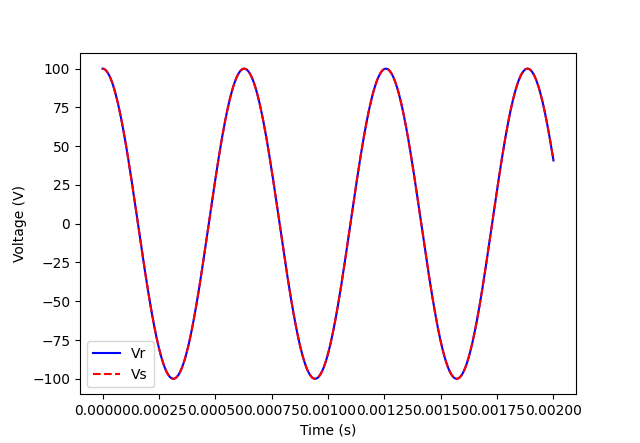
\includegraphics[width=\columnwidth]{2023/BM/42/figs/Figure42.png}
    \caption{Voltage across Resistor and Source voltage}
    \label{fig:plot42}
\end{figure}

\newpage

\item For a regular sinusoidal wave propagating in deep water having wave height of 3.5 m and wave period of 9 s, the wave steepness is \underline{\hspace{1cm}} (round off to three decimal places).
\hfill Gate 2023 NM 33\\
\solution
\input{2023/NM/33/g2.tex}
\newpage

\item  A spring mass system is shown in the figure . Take the value of acceleration  due to gravity as $g=9.81m/s^2$.The static deflection due to weight and the time period of the oscillations,respectively,are\\
 \begin{figure}[h!]
    \centering
    \includegraphics[width = \columnwidth]{2023/XE/71/figs/fig1.jpg}
\end{figure}
\hfill{(GATE 2023 XE)}\\
\solution
\input{2023/XE/71/assignment5.tex}
\pagebreak

\item In the circuit shown below, the amplitudes of the voltage across the resistor and the capacitor are equal. What is the value of the angular frequency $\omega_o$ (in rad/s)? 
(Round off the answer to one decimal place.) \hfill(GATE BM 32 2023)
\begin{circuitikz}
    % Voltage source
    \draw (0,0) to[sV, v=$100\cos(\omega_{o} t)$] (0,2);
    
    % Resistor
    \draw (0,2) to[R, l=$1\text{ k}\Omega$] (3,2);
    
    % Capacitor
    \draw (3,2) to[C, l=$100\mu\text{F}$] (3,0);
    
    % Ground
    \draw (3,0) -- (0,0);
\end{circuitikz}
\solution
\iffalse
\let\negmedspace\undefined
\let\negthickspace\undefined
\documentclass[journal,12pt,twocolumn]{IEEEtran}
\usepackage{cite}
\usepackage{amsmath,amssymb,amsfonts}
\usepackage{graphicx}
\usepackage{textcomp}
\usepackage{xcolor}
\usepackage{txfonts}
\usepackage{listings}
\usepackage{enumitem}
\usepackage{mathtools}
\usepackage{gensymb}
\usepackage{comment}
\usepackage[breaklinks=true]{hyperref}
\usepackage{tkz-euclide} 
\usepackage{listings}
\usepackage{gvv}                                        
\def\inputGnumericTable{}                                 
\usepackage[latin1]{inputenc}                                
\usepackage{color}                                            
\usepackage{array}                                            
\usepackage{longtable}                                       
\usepackage{calc}                                             
\usepackage{multirow}                                         
\usepackage{hhline}                                           
\usepackage{ifthen}                                           
\usepackage{lscape}
\usepackage[export]{adjustbox}

\newtheorem{theorem}{Theorem}[section]
\newtheorem{problem}{Problem}
\newtheorem{proposition}{Proposition}[section]
\newtheorem{lemma}{Lemma}[section]
\newtheorem{corollary}[theorem]{Corollary}
\newtheorem{example}{Example}[section]
\newtheorem{definition}[problem]{Definition}
\newcommand{\BEQA}{\begin{eqnarray}}
\newcommand{\EEQA}{\end{eqnarray}}
\newcommand{\define}{\stackrel{\triangle}{=}}
\newtheorem{rem}{Remark}

\begin{document}
\parindent 0px
\bibliographystyle{IEEEtran}

\vspace{3cm}

\title{}
\author{EE23BTECH11042 -  Khusinadha Naik$^{*}$
}
\maketitle
\newpage
\bigskip

% \renewcommand{\thefigure}{\theenumi}
% \renewcommand{\thetable}{\theenumi}


\noindent \textbf{26.} \hspace{2pt}A causal, discrete time system is described by the difference equation $y[n] = 0.5 y[n-1] + x[n]$, for all $n$, where $y[n]$ denotes the output sequence and $x[n]$ denotes the input sequence. Which of the following statements is/are TRUE?
\begin{flushright}
\hfill(GATE 2023 BM)
\end{flushright}
\begin{enumerate}[label = (\alph*)]
	\item The system has an impulse response described by $0.5^{n} u[-n]$ where $u[n]$ is the  
unit step sequence. 	\label{option:GATE.2023.BM.26.1}	
	\item The system is stable in the bounded input, bounded output sense.		\label{option:GATE.2023.BM.26.2}
	\item The system has an infinite number of non-zero samples in its impulse response	\label{option:GATE.2023.BM.26.3}
	\item The system has a finite number of non-zero samples in its impulse response.	\label{option:GATE.2023.BM.26.4}
\end{enumerate}

\noindent \textbf{Ans.}\\
\fi
\begin{table}[h]
\centering
\begin{tabular}{|c|c|c|}
        \hline
        \textbf{Parameter} & \textbf{Value} & \textbf{Description} \\
        \hline
        $x[n]$ & ? & Input Sequence \\
        \hline
        $y[n]$ & ? & Output Sequence \\
        \hline
\end{tabular}
\caption{Input parameters table}
\label{tab:GATE.2023.BM.26.1}





\end{table}
\begin{align}
y[n] = 0.5y[n-1] + x[n] 
\end{align}

Taking $Z$-Transform 
\begin{align}
Y\brak{z} &= 0.5z^{-1}Y\brak{z} + X\brak{z} \\
\implies \frac{Y\brak{z}}{X\brak{z}} &= \frac{1}{1 - 0.5z^{-1}} = H\brak{z} 
\end{align}
If $x[n]$ is impulse input 
\begin{align}
\implies &Y\brak{z} = H\brak{z} = \frac{1}{1 - 0.5z^{-1}}  \label{eq:GATE.2023.BM.26.4}
\end{align}
From \eqref{eq:GATE.2023.BM.26.4} pole lies at $z = 0.5$
\begin{align}
a^{n}u\brak{n} \xleftrightarrow{\mathcal{Z}} &\frac{1}{1 - az^{-1}} \quad , \abs{z} > a \label{eq:GATE.2023.BM.26.5}
\end{align}

From \eqref{eq:GATE.2023.BM.26.4} , \eqref{eq:GATE.2023.BM.26.5}
\begin{align}
h[n] = 0.5^{n}u[n] \quad , \abs{z} > 0.5 \label{eq:GATE.2023.BM.26.6}
\end{align}


\pagebreak
Plotting $h[n]$ vs $n$
\begin{figure}[h]
    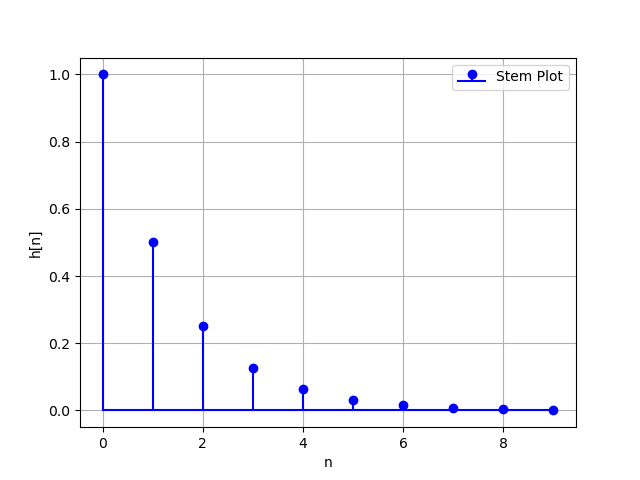
\includegraphics[width=0.5\textwidth]{2023/BM/26/figs/fig1.png}
    \caption{Plot of $h[n]$ vs $n$}
    \label{fig:GATE.2023.BM.26.1}
\end{figure}

\begin{enumerate}
\item From \eqref{eq:GATE.2023.BM.26.6} , \ref{option:GATE.2023.BM.26.1} is wrong
\item As pole lies within unit circle \ref{option:GATE.2023.BM.26.2} is true
\item From \eqref{eq:GATE.2023.BM.26.6} and \figref{fig:GATE.2023.BM.26.1} ,\ref{option:GATE.2023.BM.26.3} is true and hence
\item \ref{option:GATE.2023.BM.26.4} is false 
\end{enumerate}





%\end{document}

\pagebreak
\item Let $ w ^{4} = 16j $. Which of the fo
    llowing can not be the value of w?\\\
    \
 52 (A)   $2e^\frac{j2 \pi}{8}$\\
 53 (B)   $2e^\frac{j \pi}{8}$\\
 54 (C)   $2e^\frac{j5 \pi}{8}$\\
 55 (D)   $2e^\frac{j9 \pi}{8}$\\
\hfill{(GATE 2023 EC)}\\               \solution                              \input{2023/EC/13/gateec131.tex}     \pagebreak
\item In the diagram shown, the frequency of the sinusoidal source voltage $V_s$ is 50 Hz.The load voltage is 230 V (RMS), and the load impedance is $\frac{230}{\sqrt{2}}$+$j\frac{230}{\sqrt{2}}$ $\Omega$. The value of attenuator $A_1$=$\frac{1}{50\sqrt{2}}$.The multiplier output voltage $V_o=\frac{V_xV_y}{1V}$, where $V_x$ and $V_y$ are the inputs. The magnitude of the average value of the multiplier output $V_0$ is \hspace{3cm}\rule{5cm}{0.4pt} V

\vspace{1cm}

\begin{circuitikz}
    \draw (0,0) to[sV, l=$V_s$] (0,3) -- (6,3) ;
    \draw [european](6,3) to[R, l=Load ](6,0)  --(2,0)  ;
     \draw (5.4,0) to  (5.1,0);
    \draw (2,0) to[R, l=$1 \Omega$]   (0,0);
    \draw (5.25,3) to (5.25,-4.75) -- (4.25,-4.75) ;
    \draw  (4.25,-4) rectangle (3.25,-5) node [midway] {$A_1$};
    \draw (0,0) node[ground]{};
    \draw (4.75,0) to (4.75,-4.35) -- (4.25,-4.35);
   \draw (3.25,-4.5) to (3,-4.5);
    \draw (3,-4) rectangle(-0.5, -5) node [midway] {$+90^\circ$ phase  
    shifter};
    \draw (2.5,-4) to (2.5,-3.5) -- (3, -3.5)-- (3,-2.5) -- (2.5, -1.6339746) --(2,-2.5) -- (2,-3.5) -- (2.5,-3.5); 
    \node at (2.25,-3.75) {$V_y$};
    \draw (2, -2.5) to (3, -3.5);
    \draw (3,-2.5) to (2,-3.5) ;
    \draw (4,0) to (4,-3.25) -- (3,-3.25);
     \node at (3.25,-3) {$V_x$};
    \draw (2.5, -1.3)   to   (2.5, -1.6339746) ;
    \node at (2.15,-1.3) {$V_o$};
\end{circuitikz}

\vspace{2cm}		
\hfill{GATE 2023 IN}	
\solution\\
\iffalse
\let\negmedspace\undefined
\let\negthickspace\undefined
\documentclass[journal,12pt,twocolumn]{IEEEtran}
\usepackage{cite}
\usepackage{amsmath,amssymb,amsfonts,amsthm}
\usepackage{algorithmic}
\usepackage{graphicx}
\usepackage{textcomp}
\usepackage{xcolor}
\usepackage{txfonts}
\usepackage{listings}
\usepackage{enumitem}
\usepackage{mathtools}
\usepackage{gensymb}
\usepackage{comment}
\usepackage[breaklinks=true]{hyperref}
\usepackage{tkz-euclide} 
\usepackage{listings}
\usepackage{gvv}  
\usepackage{circuitikz}
\usetikzlibrary{intersections}
\usepackage{tikz}
\def\inputGnumericTable{}                                 
\usepackage[latin1]{inputenc}                                
\usepackage{color}                                            
\usepackage{array}                                            
\usepackage{longtable}                                       
\usepackage{calc}                                             
\usepackage{multirow}                                         
\usepackage{hhline}                                           
\usepackage{ifthen}                                           
\usepackage{lscape}


\newtheorem{theorem}{Theorem}[section]
\newtheorem{problem}{Problem}
\newtheorem{proposition}{Proposition}[section]
\newtheorem{lemma}{Lemma}[section]
\newtheorem{corollary}[theorem]{Corollary}
\newtheorem{example}{Example}[section]
\newtheorem{definition}[problem]{Definition}
\newcommand{\BEQA}{\begin{eqnarray}}
\newcommand{\EEQA}{\end{eqnarray}}
\newcommand{\define}{\stackrel{\triangle}{=}}
\theoremstyle{remark}
\newtheorem{rem}{Remark}

\begin{document}
\bibliographystyle{IEEEtran}
\vspace{3cm}
\title{\textbf{IN-2023}}
\author{EE23BTECH11053-R.Rahul$^{*}$% <-this % stops a space
}
\maketitle
\newpage
\bigskip

\textbf{QUESTION:}\\
61. In the diagram shown, the frequency of the sinusoidal source voltage $V_s$ is 50 Hz.The load voltage is 230 V (RMS), and the load impedance is $\frac{230}{\sqrt{2}}$+$j\frac{230}{\sqrt{2}}$ $\Omega$. The value of attenuator $A_1$=$\frac{1}{50\sqrt{2}}$.The multiplier output voltage $V_o=\frac{V_xV_y}{1V}$, where $V_x$ and $V_y$ are the inputs. The magnitude of the average value of the multiplier output $V_0$ is \hspace{3cm}\rule{5cm}{0.4pt} V

\vspace{1cm}

\begin{circuitikz}
    \draw (0,0) to[sV, l=$V_s$] (0,3) -- (6,3) ;
    \draw [european](6,3) to[R, l=Load ](6,0)  --(2,0)  ;
     \draw (5.4,0) to  (5.1,0);
    \draw (2,0) to[R, l=$1 \Omega$]   (0,0);
    \draw (5.25,3) to (5.25,-4.75) -- (4.25,-4.75) ;
    \draw  (4.25,-4) rectangle (3.25,-5) node [midway] {$A_1$};
    \draw (0,0) node[ground]{};
    \draw (4.75,0) to (4.75,-4.35) -- (4.25,-4.35);
   \draw (3.25,-4.5) to (3,-4.5);
    \draw (3,-4) rectangle(-0.5, -5) node [midway] {$+90^\circ$ phase  
    shifter};
    \draw (2.5,-4) to (2.5,-3.5) -- (3, -3.5)-- (3,-2.5) -- (2.5, -1.6339746) --(2,-2.5) -- (2,-3.5) -- (2.5,-3.5); 
    \node at (2.25,-3.75) {$V_y$};
    \draw (2, -2.5) to (3, -3.5);
    \draw (3,-2.5) to (2,-3.5) ;
    \draw (4,0) to (4,-3.25) -- (3,-3.25);
     \node at (3.25,-3) {$V_x$};
    \draw (2.5, -1.3)   to   (2.5, -1.6339746) ;
    \node at (2.15,-1.3) {$V_o$};
\end{circuitikz}

\vspace{2cm}		
	
\solution
\fi
\begin{table}[h]
  \centering
  \renewcommand{\arraystretch}{1.5}
\begin{tabular}{|c|c|c|}
\hline
Parameter & Description & Value \\\hline
\( V_s \) & sinusoidal Source voltage & 230 V(RMS)\\ \hline
\(V_1 \) & voltage across attenuator &  \\\hline
\( V_x and V_y \) & inputs voltages& \\ \hline
\(A_1\) & attenuator&  $\frac{1}{50\sqrt{2}}$ \\ \hline
\(Z\) & Load Impedance& $\frac{230}{\sqrt{2}}+j\frac{230}{\sqrt{2}}$ $\Omega$ \\ \hline
\(V_0\) & output voltage & $V_0=\frac{V_xV_y}{1V} $\\ \hline
\end{tabular}
\caption{variables}
  \label{tab:xn}
\end{table}
\begin{enumerate}
    \item 

Let the curret in load be I

\begin{center}
\begin{align}
     I &=\frac{V_s(peak)}{Z}\\
     &=\frac{230\sqrt{2}}{\frac{230}{\sqrt{2}}+j\frac{230}{\sqrt{2}}} \\
     &=\sqrt{2}(1-j)
\end{align}
\end{center}
\item
voltage at attenuator 
\begin{align}
    V_1&=V_sA_1\\
    &=230\frac{1}{50\sqrt{2}}V\\
    &=\frac{4.6}{\sqrt{2}}V
\end{align}

\begin{center}
    \begin{align}
        V_y&=4.6\sin(\omega t+90^\circ)\\
        V_x&=I\times 1\Omega\\
        &=2\sqrt{2}\sin(\omega t-45^\circ)\\
        V_0&=9.2\sqrt{2}(\frac{\cos(135)-\cos(2\omega t)}{2})\\
        &=4.6-4.6\sqrt{2}\cos(2\omega t)\\
    \end{align}
\end{center}

\item 
Let f(t)= $4.6-4.6\sqrt{2}\cos(2\omega t)$
\begin{align}
    V_o<avg>&=\frac{1}{T}\int_{0}^{T}(4.6-4.6\sqrt{2}\cos(2\omega t))\,dt\\
    &=\frac{\omega}{\pi} \left[\int_{0}^{\frac{\pi}{\omega}}4.6\,dt-4.6\sqrt{2}\int_{0}^{\frac{\pi}{\omega}}\cos(2\omega t)\,dt\right]\\
    &=\frac{\omega}{\pi}\left[4.6\frac{\pi}{\omega}-4.6\sqrt{2}\left[\frac{\sin(2\pi )}{2\omega}\right]\right]\\
    &=4.6
\end{align}
\end{enumerate}
\begin{figure}[h]
      \centering
       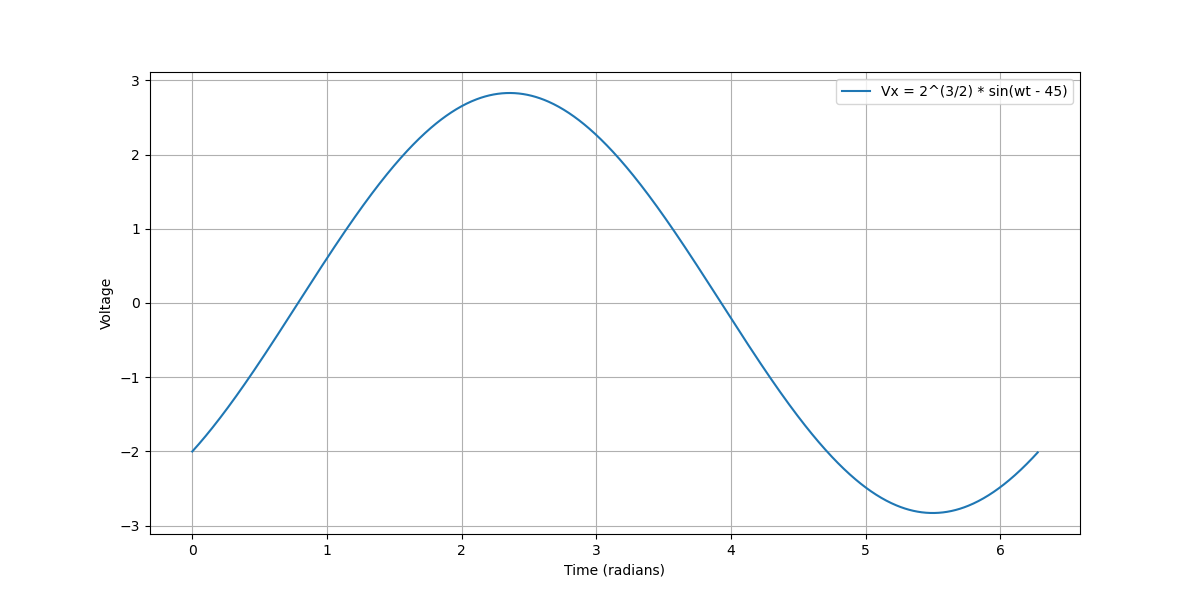
\includegraphics[width=1\linewidth]{2023/IN/61/figs/V_x.png} % Adjust the width as needed
        \caption{$plot of V_x$}
\end{figure}
\begin{figure}[h]
      \centering
       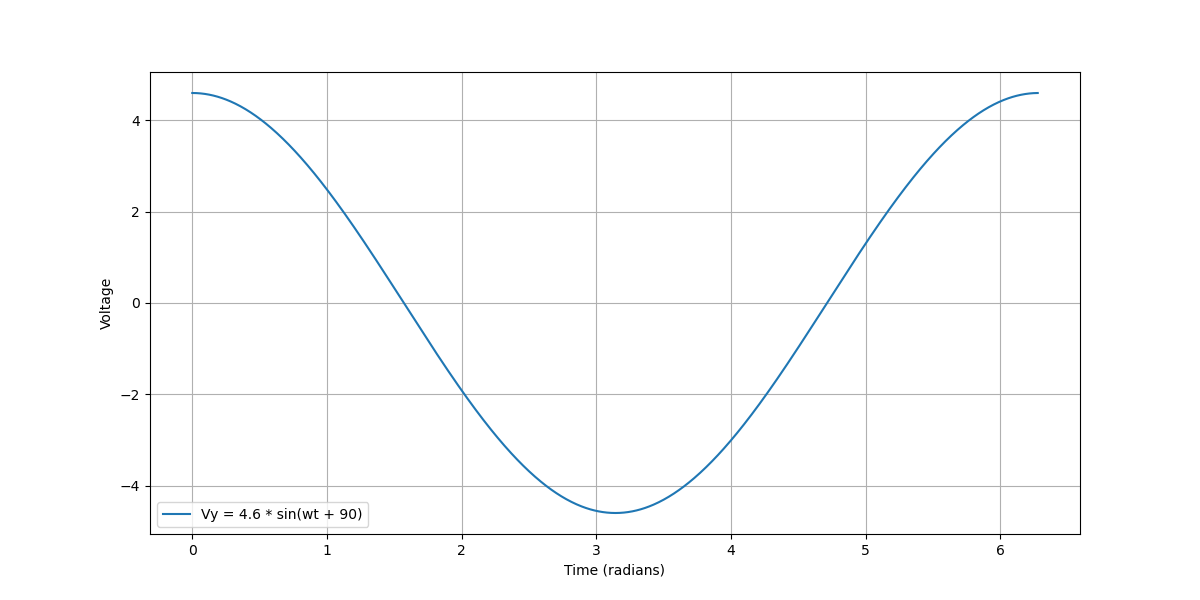
\includegraphics[width=1\linewidth]{2023/IN/61/figs/V_y.png} % Adjust the width as needed
        \caption{$plot of V_y$}
\end{figure}
\begin{figure}[h]
      \centering
       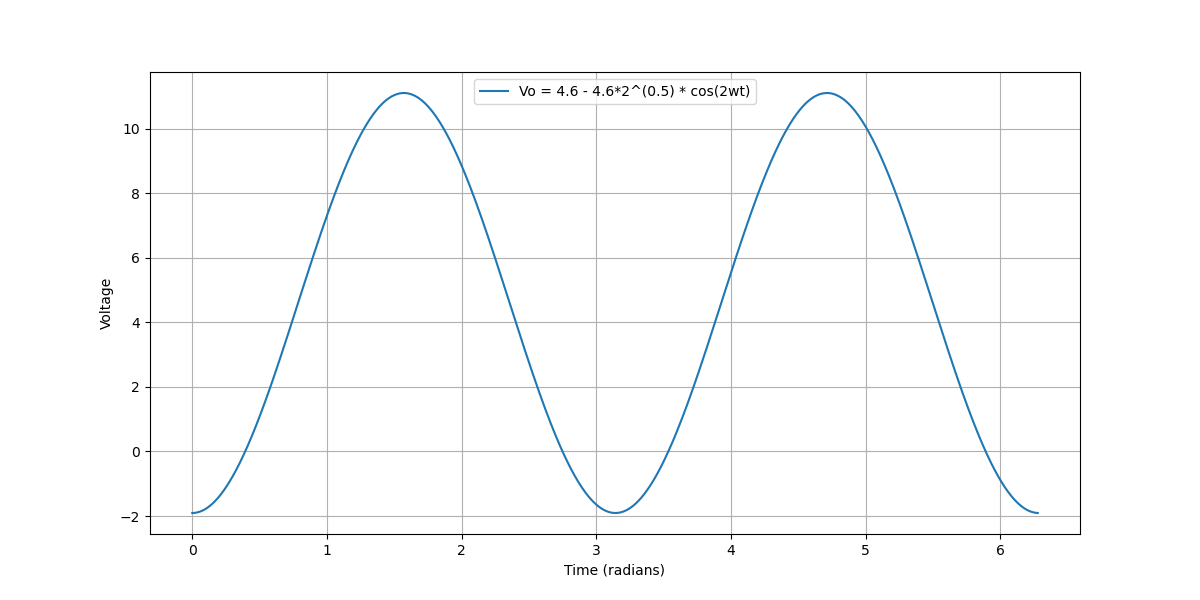
\includegraphics[width=1\linewidth]{2023/IN/61/figs/V_o.png} % Adjust the width as needed
        \caption{$plot of V_o$}
\end{figure}
%\end{document}

\end{enumerate}

\chapter{Filters}
\begin{enumerate}[label=\thechapter.\arabic*,ref=\thechapter.\theenumi]
\item
For the circuit given below, choose the angular frequency $ \omega_0$ at which voltage across capacitor has maximum amplitude?
\begin{figure}[h!]
    \includegraphics[width = 0.5\columnwidth]{2023/BM/16/figs/c_fig1.pdf}
    \caption{circuit }
    \centering
    \label{fig: bm_16_fig_1}
\end{figure}
\begin{enumerate}
    \item[(A)] 1000
    \item[(B)] 100
    \item[(C)] 1
    \item[(D)] 0   
\end{enumerate}
\hfill(GATE BM 2023 Question 16)\\

\solution
\input{2023/BM/16/asnmt3.tex}
\newpage
\item
In the following circuit, the switch S is open for $t < 0$ and closed for $t \ge 0$.
What is the steady state voltage (in Volts) across the capacitor when the switch is closed?
\begin{figure}[h!]
    \includegraphics[width = 0.7\columnwidth]{2023/BM/30/figs/c_fig1.pdf}
    \caption{circuit }
    \centering
    \label{fig:bm_30_fig_1}
\end{figure}
\hfill(GATE BM 2023 Question 30) \\
\solution
\iffalse
\let\negmedspace\undefined
\let\negthickspace\undefined
\documentclass[journal,12pt,twocolumn]{IEEEtran}
\usepackage{cite}
\usepackage{amsmath,amssymb,amsfonts,amsthm}
\usepackage{algorithmic}
\usepackage{graphicx}
\usepackage{textcomp}
\usepackage{xcolor}
\usepackage{txfonts}
\usepackage{listings}
\usepackage{enumitem}
\usepackage{mathtools}
\usepackage{gensymb}
\usepackage{comment}
\usepackage[breaklinks=true]{hyperref}
\usepackage{tkz-euclide}
\usepackage{listings}
\usepackage{gvv}
\def\inputGnumericTable{}
\usepackage[latin1]{inputenc}
\usepackage{color}
\usepackage{array}
\usepackage{longtable}
\usepackage{calc}
\usepackage{multirow}
\usepackage{hhline}
\usepackage{ifthen}
\usepackage{lscape}

\newtheorem{theorem}{Theorem}[section]
\newtheorem{problem}{Problem}
\newtheorem{proposition}{Proposition}[section]
\newtheorem{lemma}{Lemma}[section]
\newtheorem{corollary}[theorem]{Corollary}
\newtheorem{example}{Example}[section]
\newtheorem{definition}[problem]{Definition}
\newcommand{\BEQA}{\begin{eqnarray}}
\newcommand{\EEQA}{\end{eqnarray}}
\newcommand{\define}{\stackrel{\triangle}{=}}
\theoremstyle{remark}
\newtheorem{rem}{Remark}
\begin{document}

\bibliographystyle{IEEEtran}
\vspace{3cm}

\title{GATE 2023 BM 30}
\author{EE23BTECH11007 - Aneesh Kadiyala$^{*}$% <-this % stops a space
}
\maketitle
\newpage
\bigskip

\renewcommand{\thefigure}{\theenumi}
\renewcommand{\thetable}{\theenumi}

\vspace{3cm}
\textbf{Question:} In the following circuit, the switch S is open for $t < 0$ and closed for $t \ge 0$.
What is the steady state voltage (in Volts) across the capacitor when the switch is closed?
\begin{figure}[h!]
    \centering
    \includegraphics[width = \columnwidth]{2023/BM/30/figs/c_fig1.pdf}
\end{figure}
\\
\solution
\\
\fi
\begin{figure}[h!]
    \centering
    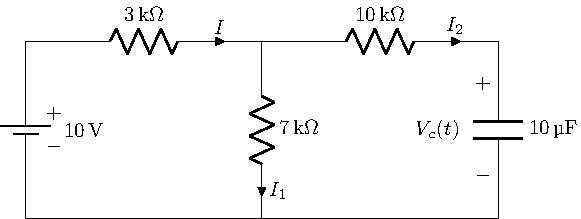
\includegraphics[width=\columnwidth]{2023/BM/30/figs/c_fig3.pdf}
\end{figure}
\\
In steady state, no current flows through the capacitor.
\begin{align}
I_2 &= 0 \\
V_c &= \brak{7\text{k}\ohm}I_1 \\
&= \brak{7\text{k}\ohm}I \\
&= \brak{7\text{k}\ohm}\frac{10\text{V}}{10\text{k}\ohm} \\
\implies V_c &= 7\text{V}
\end{align}
In s-domain:
\begin{figure}[h!]
    \centering
    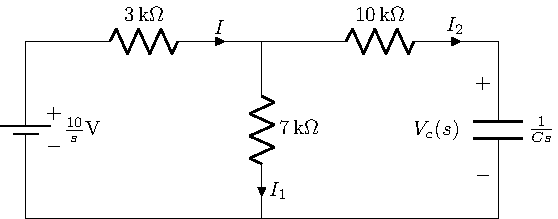
\includegraphics[width=\columnwidth]{2023/BM/30/figs/c_fig2.pdf}
\end{figure}
\begin{align}
\implies I\brak{s} &= \frac{\frac{10}{s}\text{V}}{3\text{k}\ohm + \frac{(7\text{k}\ohm)(10\text{k}\ohm + \frac{1}{sC})}{17\text{k}\ohm + \frac{1}{sC}}} \\
I &= I_1 + I_2 \\
I_1\brak{7\text{k}\ohm} &= I_2\brak{10\text{k}\ohm + \frac{1}{sC}} \\
I_2\brak{s} &= \frac{7\text{k}\ohm}{17\text{k}\ohm + \frac{1}{sC}}I\brak{s} \\
%&= \frac{\frac{70000}{s}}{121 * 10^6 + \frac{10000}{sC}} \\
%&= \frac{\frac{7}{s}}{121 * 10^2 + \frac{1}{sC}} \\
\implies I_2\brak{s} &= \frac{7\brak{10^{-5}}}{0.121s + 1} \\
V_c\brak{s} &= I_2\brak{s}\frac{1}{sC} \\
&= \frac{7}{s\brak{0.121s + 1}} \\
%&= 7\brak{\frac{\frac{1}{0.121}}{s\brak{s + \frac{1}{0.121}}}} \\
&= 7\brak{\frac{1}{s} - \frac{1}{s + \frac{1}{0.121}}}
\end{align}
Taking inverse Laplace transform:
\begin{align}
V_c\brak{t} &= 7u\brak{t}\brak{1 - e^{-\frac{t}{-0.121}}} \label{eq:2023BM30}
\end{align}
\begin{figure}[h!]
\centering
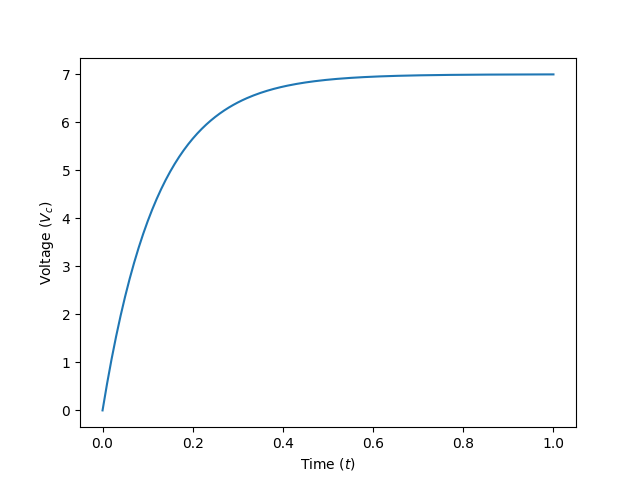
\includegraphics[width=\columnwidth]{2023/BM/30/figs/plot.png}
%\caption{$V_c$ vs $t$}
\label{fig:2023BM30}
\end{figure}
\\
In steady state $t \to \infty$. From \eqref{eq:2023BM30}:
\begin{align}
\lim_{t\to\infty}V_c\brak{t} &= 7\text{V}
\end{align}

\pagebreak
\item 
A finite impulse response (FIR) filter has only two non-zero samples in its impulse response $h[n]$, namely $h[0] = h[1] = 1$. The Discrete Time Fourier Transform (DTFT) of $h[n]$ equals $H(e^{j\omega})$, as a function of the normalized angular frequency $\omega$. For the range $\abs{\omega} \leq \pi$, $\abs{H(e^{j\omega})}$ is equal to
\begin{enumerate}
	\item[(A)] $2\abs{\cos(\omega)}$
	\item[(B)] $2\abs{\sin(\omega)}$
	\item[(C)] $2\abs{\cos(\frac{\omega}{2})}$
	\item[(D)] $2\abs{\sin(\frac{\omega}{2})}$
\end{enumerate}
\hfill(GATE BM 2023 Question 17) \\
\solution
\input{2023/BM/17/1.tex}
\pagebreak
\item
For the circuit shown,if $i=\sin 1000t$, the instantaneous value of the Thevenin's voltage(in volts) across the terminals a anb b at time t=5ms is\\[2pt]

\begin{circuitikz}[american voltages,american currents]
    % Draw the circuit components
    \draw (0,0) -- (2,0);
    \draw (2,2) to [resistor,l=$10\Omega$] (2,4);
    \draw (2,4) -- (0,4);
    \draw (2,0) to [capacitor,l=$-j10\Omega$,-,i_=$i_x$] (2,2);
    \draw (2,0) -- (5,0);
    \draw (5,0) to[inductor,l=$j10\Omega$] (5,2);
    \draw (5,2) to [resistor,l=$10\Omega$] (5,4);
  \draw (5,4) to [cV,l^=$4i_x$,invert] (2,4);
  \draw (5,4) -- (6,4);
  \draw (6,4) to[I,l=$\sin 1000t$,invert] (6,0);
  \draw (6,0) -- (5,0);
   \node[circle,fill=black,inner sep=1.5pt,label=above:a] at (0,0) {};
    \node[circle,fill=black,inner sep=1.5pt,label=above:b] at (0,4) {};
    \end{circuitikz}
    \hfill(GATE EE 2023 ) \\
    \solution
    \input{2023/EE/51/gate51.2023.tex}
    \pagebreak

    \item In the circuit shown ,$\omega=100\pi\text{rads/s}$, R1=R2=$2.2\Omega$ and L=$7\text{mH}$. the capacitance $\text{C}$ for which $Y_{in}$ is purely real is  $\text{mF}$ \\
	\begin{center}
	\begin{circuitikz} \centering \draw 
		(0,4) to[sinusoidal voltage source, l=$V_{0}$cos($\omega$t)] (0,0)
		(0,4) to[short] (4,4)
		(4,4) to[resistor, l=$R_1$ ] (4,2)
		(4,2) to[inductor, l= $\text{L} $] (4,0) to[short ] (0,0)
		(8,4)  to[short] (4,4)
		(8,4) to[resistor, l= $R_2$] (8,2) to[capacitor,l=$\text{C}$] (8,0) to (4,0);
	\end{circuitikz}
	\end{center}
\hfill(GATE IN 2023 Q46)\\
\solution
\input{2023/IN/46/7.tex}

\pagebreak
\item An input voltage in the form of a square wave of frequency $1\, kHz$ is given to a circuit, which results in the output shown schematically below. Which one of the following options is the CORRECT representation of the circuit? \hfill(GATE PH 2023 Q37)
\begin{figure}[!h]
    \centering
    \includegraphics[width = 0.6\columnwidth]{2023/PH/37/figs/question.png}
	\caption{}\
	\label{fig:ques_gate.ph.23.37}
\end{figure}

\begin{enumerate}[label = (\alph*)]
    \item 
    \begin{figure}[!h]
        \centering
	    \resizebox{0.2\textwidth}{!}{\input{2023/PH/37/figs/optA}}
	\label{optA_gate.ph.23.37}
    \end{figure}

    \item 
    \begin{figure}[!h]
        \centering
        \resizebox{0.2\textwidth}{!}{\input{2023/PH/37/figs/optB}}
        \label{optB_gate.ph.23.37}
    \end{figure}

    \item 
    \begin{figure}[!h]
        \centering
        \resizebox{0.2\textwidth}{!}{\input{2023/PH/37/figs/optC}}
        \label{optC_gate.ph.23.37}
    \end{figure}

    \item 
    \begin{figure}[!h]
        \centering
        \resizebox{0.2\textwidth}{!}{\input{2023/PH/37/figs/optD}}
        \label{optD_gate.ph.23.37}
    \end{figure}
\end{enumerate} \hfill(GATE 2023 PH 37)\\
\solution
\input{2023/PH/37/GATE_PH_23_37.tex}
\pagebreak

\item In the circuit shown below, switch S was closed for long time. If the switch is opened at $t=0$, the  maximum magnitude of the voltage $V_R$ , in volts is (rounded off to the nearest integer)\hfill{(GATE 2023 EC 35)}\\
\begin{figure}[h!]
    \centering
    \includegraphics[width=1\linewidth]{2023/EC/35/figs/gate.png}
    \caption{ }
\end{figure}
\solution
\input{2023/EC/35/assign3.tex}
\pagebreak
\item A signal $x\brak{t}=2\cos{(180\pi t)}\cos{(60\pi t)}$ is sampled at 200 Hz and then passed through an ideal low pass filter having cut-off frequency of 100 Hz.\\
The maximum Frequency present in the filtered  signal in Hz is \rule{1cm}{0.5mm} (Round off to the nearest integer.) \hfill (GATE 2023 EE)
\solution
\iffalse
\let\negmedspace\undefined
\let\negthickspace\undefined
\documentclass[journal,12pt,twocolumn]{IEEEtran}
\usepackage{cite}
\usepackage{amsmath,amssymb,amsfonts}
\usepackage{graphicx}
\usepackage{textcomp}
\usepackage{xcolor}
\usepackage{txfonts}
\usepackage{listings}
\usepackage{enumitem}
\usepackage{mathtools}
\usepackage{gensymb}
\usepackage{comment}
\usepackage[breaklinks=true]{hyperref}
\usepackage{tkz-euclide} 
\usepackage{listings}
\usepackage{gvv}                                        
\def\inputGnumericTable{}                                 
\usepackage[latin1]{inputenc}                                
\usepackage{color}                                            
\usepackage{array}                                            
\usepackage{longtable}                                       
\usepackage{calc}                                             
\usepackage{multirow}                                         
\usepackage{hhline}                                           
\usepackage{ifthen}                                           
\usepackage{lscape}
\usepackage[export]{adjustbox}
\usepackage{pgfplots}
\newtheorem{theorem}{Theorem}[section]
\newtheorem{problem}{Problem}
\newtheorem{proposition}{Proposition}[section]
\newtheorem{lemma}{Lemma}[section]
\newtheorem{corollary}[theorem]{Corollary}
\newtheorem{example}{Example}[section]
\newtheorem{definition}[problem]{Definition}
\newcommand{\BEQA}{\begin{eqnarray}}
	\newcommand{\EEQA}{\end{eqnarray}}
\newcommand{\define}{\stackrel{\triangle}{=}}
\newtheorem{rem}{Remark}

\begin{document}
	\parindent 0px
	\bibliographystyle{IEEEtran}
	
	\vspace{3cm}
	
	\title{GATE:EE/63}
	\author{EE23BTECH11208 - Manohar K$^{*}$
	}
	\maketitle
	\newpage
	\bigskip
	
	% \renewcommand{\thefigure}{\theenumi}
	% \renewcommand{\thetable}{\theenumi}
	
	
	
	\textbf{Question:} \hspace{2pt} A signal $x\brak{t}=2\cos{(180\pi t)}\cos{(60\pi t)}$ is sampled at 200 Hz and then passed through an ideal low pass filter having cut-off frequency of 100 Hz.\\
	The maximum Frequency present in the filtered  signal in Hz is \rule{1cm}{0.5mm} (Round off to the nearest integer.) \hfill (GATE 2023 EE)\\
	\noindent \textbf{Solution:}\\
\fi
	\begin{figure}[ht]
		\centering
		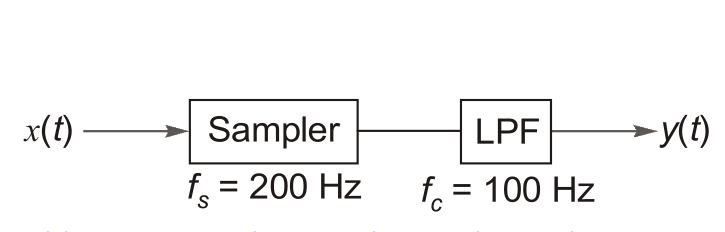
\includegraphics[width=1\linewidth]{2023/EE/63/figs/answerdia.png}
	\end{figure}
	Given, \\
	
	\begin{align}
		x\brak{t}&=\cos\brak{240\pi t} + \cos\brak{120\pi t}
	\end{align}\\
	\begin{table}[h]
		\centering
		
\begin{tabular}{|c|c|c|}
	\hline
	\textbf{symbol} & \textbf{value} & \textbf{description} \\
	\hline
	$x(t)$ & $2\cos{(180\pi t)}\cos{(60\pi t)}$ & input signal \\
	\hline
	$f_s$ & $200Hz$ & sampling frequency \\
	\hline
	$f_c$ & $100Hz$ & cut-off frequency \\
	\hline
	$y(t)$ &  & output signal \\
	\hline
	$f_1$ & $120Hz$ & first signal frequency \\
	\hline
	$f_2$ & $60Hz$ & second signal frequency \\
	\hline
\end{tabular}

		\caption{Parameters}
		\label{tab:GATE.EE.2023.63}
	\end{table}\\
	Aliased frequencies when $f_1$ frequency signal is sampled at $200Hz$\\
	\begin{align}
		& f_1 , \abs{f_s\pm f_1} , \abs{2f_s \pm f_1} \dots\\
		& 120, 80,340,280,520 \dots
	\end{align}
	Aliased frequencies when $f_2$ frequency signal is sampled at $200Hz$\\
	\begin{align}
		& f_2 , \abs{f_s\pm f_2} , \abs{2f_s\pm f_2} \dots\\
		& 60 , 140,260,340,460 \dots 
	\end{align}
\begin{figure}
	\centering
	\begin{tikzpicture}
\begin{axis}[
    axis lines=middle,
    xlabel=$f$,
    ylabel=$X(f)$,
    ymax=1,
    ymin=0,
    xmin=-240,
    xmax=240,
    xtick={ -120, -60, 60, 120},
    ytick={0,1},
    yticklabels={0,1},
    ticklabel style={font=\tiny},
    enlargelimits={abs=0.2},
    clip=false
]
% One-sided arrows
\draw[->, >=latex, blue, thick] (axis cs: -120, 0) -- (axis cs: -120, 1);
\draw[->, >=latex, blue, thick] (axis cs: -60, 0) -- (axis cs: -60, 1);
\draw[->, >=latex, blue, thick] (axis cs: 60, 0) -- (axis cs: 60, 1);
\draw[->, >=latex, blue, thick] (axis cs: 120, 0) -- (axis cs: 120, 1);
\end{axis}
\end{tikzpicture}

	\caption{delta function of input signal }
\end{figure}\\
	
	
\begin{figure}
	\centering
	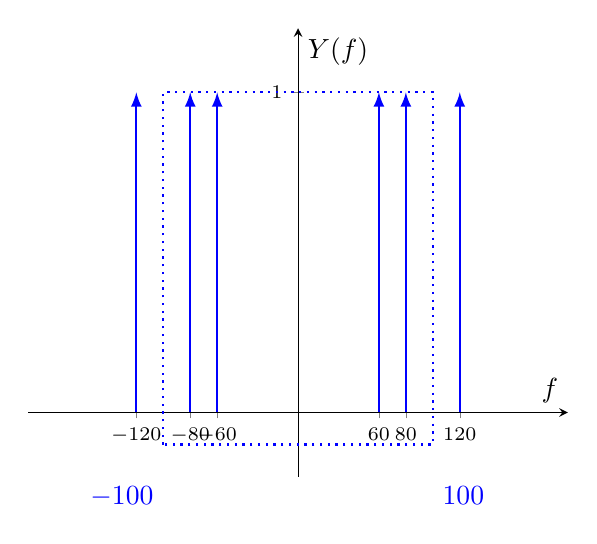
\begin{tikzpicture}
\begin{axis}[
    axis lines=middle,
    xlabel=$f$,
    ylabel=$Y(f)$,
    ymax=1,
    ymin=0,
    xmin=-200,
    xmax=200,
    xtick={ -120, -80, -60, 60, 80, 120},
    ytick={0,1},
    yticklabels={0,1},
    ticklabel style={font=\scriptsize},
    enlargelimits={abs=0.2},
    clip=false
]
% One-sided arrows
\draw[->, >=latex, blue, thick] (axis cs: -120, 0) -- (axis cs: -120, 1);
\draw[->, >=latex, blue, thick] (axis cs: -80, 0) -- (axis cs: -80, 1);
\draw[->, >=latex, blue, thick] (axis cs: -60, 0) -- (axis cs: -60, 1);
\draw[->, >=latex, blue, thick] (axis cs: 60, 0) -- (axis cs: 60, 1);
\draw[->, >=latex, blue, thick] (axis cs: 80, 0) -- (axis cs: 80, 1);
\draw[->, >=latex, blue, thick] (axis cs: 120, 0) -- (axis cs: 120, 1);
% Dotted box
\draw[blue, dotted, thick] (axis cs: -100, -0.1) rectangle (axis cs: 100, 1);
\node[blue, below right] at (axis cs: 100, -0.2) {$100$};
\node[blue, below left] at (axis cs: -100, -0.2) {$-100$};
\end{axis}
\end{tikzpicture}

	\caption{delta function of sampled and filtered signal }
\end{figure}
	from table $f_c = 100Hz$ \\
	LPF output : $60Hz$ , $80Hz$\\
	Maximum Frequency present in the filtered signal is $80Hz$.
	
	
	

\pagebreak
\item In the circuit shown, the input voltage $V_{in} = 100mV$. The switch and the opamp are ideal. At time $t=0$, the intial charge stored in the $10nF$ capacitor is $1nC$, with the polarity as indicated in the figure. The switch $S$ is controlled using a $1KHz$ square-wave voltage signal $V_s$ as shown. Whenever $V_s$ is `High', $S$ is in position $`1$' and when $V_s$ is `Low', $S$ is in position `$2$'.\\
At $t = 20ms$, the magnitude of the voltage $V_o$ will be  \\  
\begin{figure}[ht]
  \centering
    \resizebox{0.55\columnwidth}{!}{\begin{circuitikz}[american]
    \draw (0,0) to[R, l=$10K\Omega$] (2,0) to[L, l=$10mH$] (4,0) to[C, l=$1\mu{F}$] (6,0) -- (6,-1) 
    to[sV, l=$100\cos\brak{\omega_0 t}$] (0,-1) -- (0,0)
    (0,-1) node[circ]{} node[left]{$+$}
    (6,-1) node[circ]{} node[right]{$-$};
\end{circuitikz}
}
\end{figure}
\hfill{(GATE IN 2023)}\\
\solution
\pagebreak

\item The value of parameters of the circuit shown in the figure are $R_1=2\ohm$,$R_2=2\ohm$,$R_3=3\ohm$,$L=10 mH$,$C=100\mu F$. For time \(t<0\), the circuit is at steady state with the switch $ 'K'$ in closed condition. If the switch is opened at $t=0$, the value of the voltage across the inductor \brak{V_L}
 at $t=0^{+}$ in Volts is \rule{2cm}{0.4pt} (Round off to 1 decimal place).
\begin{circuitikz}
    \draw (0,0) to [R, R=$R_3$] (0,2);
    \draw (0,3) to [switch, o-o, name=$K$] (0,2);
    \draw (0,3)-- (0,4);
    \draw (0,4) -- (4,4);
    \draw (3,0) to [american current source, l=$10\,\text{A,}\text{DC}$] (3,4);
    \draw (4,4) to (4,5) to (5,5) to[R, l=$R_1$] (6,5);
    \draw (6,5) to(7,5) to[L, l=$L$] (8,5) to (9,5);
    \draw (4,4)to (4,3)to (5,3) to[R, l=$R_2$] (6,3);
    \draw (6,3)to (7,3) to [C, l=$C$] (8,3) to(9,3);
    \draw (9,5) --(9,3);
    \draw (9,4) -- (10,4);
    \draw (10,4)-- (10,0);
    \draw(10,0)--(0,0);
\end{circuitikz} \hfill (GATE 2023 EE 29Q)
\solution
\pagebreak

\item The op amps in the circuit are ideal. The input signals are $V_{S1} = 3 + 0.10 \sin(300t), \text{V}$ and $V_{S2} = -2 + 0.11 \sin(300t)\, \text{V}$. The average value of the voltage $V_0$ is \underline{\hspace{1cm}} volts (rounded off to two decimal places).
\begin{figure}[ht]
\centering
\resizebox{0.55\columnwidth}{!}{\input{2023/IN/59/figs/gate.circuit.tex}}
\end{figure}
\hfill{(GATE IN 2023)}
\solution
\let\negmedspace\undefined
\let\negthickspace\undefined
\documentclass[journal,12pt,twocolumn]{IEEEtran}
\usepackage{cite}
\usepackage{amsmath,amssymb,amsfonts,amsthm}
\usepackage{algorithmic}
\usepackage{graphicx}
\usepackage{textcomp}
\usepackage{xcolor}
\usepackage{txfonts}
\usepackage{listings}
\usepackage{enumitem}
\usepackage{mathtools}
\usepackage{gensymb}
\usepackage{comment}
\usepackage[breaklinks=true]{hyperref}
\usepackage{tkz-euclide}
\usepackage{listings}
\usepackage{gvv}
\def\inputGnumericTable{}
\usepackage[latin1]{inputenc}
\usepackage{color}
\usepackage{array}
\usepackage{longtable}
\usepackage{calc}
\usepackage{multirow}
\usepackage{hhline}
\usepackage{ifthen}
\usepackage{lscape}
\usepackage{circuitikz}

\newtheorem{theorem}{Theorem}[section]
\newtheorem{problem}{Problem}
\newtheorem{proposition}{Proposition}[section]
\newtheorem{lemma}{Lemma}[section]
\newtheorem{corollary}[theorem]{Corollary}
\newtheorem{example}{Example}[section]
\newtheorem{definition}[problem]{Definition}
\newcommand{\BEQA}{\begin{eqnarray}}
\newcommand{\EEQA}{\end{eqnarray}}
\newcommand{\define}{\stackrel{\triangle}{=}}
\theoremstyle{remark}
\newtheorem{rem}{Remark}
\begin{document}

\bibliographystyle{IEEEtran}
\vspace{3cm}

\title{Gate 2023- Instrumentation Engineering}
\author{EE23BTECH11037 - M Esha$^{*}$% <-this % stops a space
}
\maketitle
\newpage
\bigskip

\renewcommand{\thefigure}{\theenumi}
\renewcommand{\thetable}{\theenumi}

\vspace{3cm}
\textbf{Question 59:} 
The op amps in the circuit are ideal. The input signals are $V_{S1} = 3 + 0.10 \sin(300t), \text{V}$ and $V_{S2} = -2 + 0.11 \sin(300t)\, \text{V}$. The average value of the voltage $V_0$ is \underline{\hspace{1cm}} volts (rounded off to two decimal places).

\begin{figure}[ht]
\centering
\resizebox{0.55\columnwidth}{!}{\begin{circuitikz}

% Lines
\draw (-2.5,2.5) -- (0.5,2.5);
\draw (0.5,3) -- (0.5,1);
\draw (0.5,1.5) -- (0,1.5);
\draw (0,1.5) -- (0,0);
\draw (-2.5,-4) -- (0.5,-4);
\draw (0.5,-4.5) -- (0.5,-2.5);
\draw (0.5,-3) -- (0,-3);
\draw (0,-3) -- (0,-1.5);
\draw (0.5,3) -- (2,2);
\draw (0.5,1) -- (2,2);
\draw (2,2) -- (3.5,2);
\draw (3.5,2) -- (5.5,2);
\draw (3.5,2) -- (3.5,1.5);
\draw (0.5,-2.5) -- (2,-3.5);
\draw (0.5,-4.5) -- (2,-3.5);
\draw (2,-3.5) -- (3.5,-3.5);
\draw (3.5,-3.5) -- (3.5,-3);
\draw (3.5,-3.5) -- (5.5,-3.5);
\draw (5.5,-3.5) -- (5.5,-2.25);
\draw (5.5,2) -- (5.5,0.75);
\draw (5.5,-0.75) -- (6.5,-0.75);
\draw (0,0) -- (3.5,0);
\draw (0,-1.5) -- (3.5,-1.5);
\draw (6.5,-1.5) -- (6.5,-2.5);
\draw (6.25,-2.5) -- (6.75,-2.5);
\draw (6.3,-2.55) -- (6.7,-2.55);


% Resistors
\draw (3.5,1.5) to [resistor] (3.5,0);
\draw (3.5,0) to [resistor] (3.5,-1.5);
\draw (3.5,-1.5) to [resistor] (3.5,-3);
\draw (5.5,0.75) to [resistor] (5.5,-0.75);
\draw (5.5,-0.75) to [resistor] (5.5,-2.25);

% Labels
\node at (-3,2.5) {$V_{S1}$};
\node at (-3,-4) {$V_{S2}$};
\node at (0.75,2.5) {+};
\node at (0.75,1.5) {-};
\node at (0.75,-3) {-};
\node at (0.75,-4) {+};
\node at (7,-0.75) {$V_o$};
\node at (4.25,0.75) {R};
\node at (4.25,-0.75) {R};
\node at (4.25,-2.25) {R};
\node at (6.25,0) {R};
\node at (6.25,-1.5) {R};
\node at (6.75,-0.8) {+};
\node at (6.75,-1.5) {-};

% Dot 
\filldraw (6.5,-0.75) circle [radius=0.05];
\fill (6.5,-1.5) circle [radius=0.05]; 

\end{circuitikz}

}
\end{figure}
\hfill{(GATE IN 2023)}\\
\solution
\begin{table}[h!]
  \centering
  \begin{tabular}{|c|c|c|}
  \hline
  \textbf{Variable} & \textbf{Value} & \textbf{Description} \\
  \hline
  $V_{s1}$ & $3 + 0.10 \sin(300t)$ & \multirow{2}{*}{Input voltages} \\
  \cline{1-2}
  $V_{s2}$ & $-2 + 0.11 \sin(300t)$ & \\
  \cline{1-3}
  $R$ & & Resistances of the resistors \\
  \cline{1-3}
  $V_o$ & & Output voltage \\
  \cline{1-3}
  $V_1$ & & Output voltage of $V_{s1}$ opamp \\
  \cline{1-3}
  $V_2$ & & Output voltage of $V_{s2}$ opamp \\
  \hline
\end{tabular}

  \caption{Input Parameters}
    \label{tab:table1}
\end{table}\\
the current does not flow through op-amp. voltage drop by each R
\begin{align}
&= V_{s1}-V_{s2}
\end{align}
by KVL,
\begin{align}
V_{s2}-V_2&=V_{s1}-V_{s2}\\
V_2&=2V_{s2}-V_{s1}\\
V_1-V_{s1}&=V_{s1}-V_{s2}\\
V_1&= 2V_{s1}-V_{s2}\\
V_o&= \frac{V_1+V_2}{2}\\
&=\frac{V_{s1}+V_{s2}}{2}\\
&=\frac{3+0.10\sin(300t)+{-2}+0.11\sin(300t)}{2}\\
&=0.5+ \frac{0.21\sin(300t)}{2}\\
V_{avg}&=\frac{1}{T} \int_{0}^{T} V(t) \,dt\\
&=\frac{300}{2\pi} \int_{0}^{\frac{2\pi}{300}} \left(0.5 + \frac{0.21 \sin(300t)}{2}\right) \, dt\\
&=0.5
\end{align}
\begin{figure}[b]
    \centering
    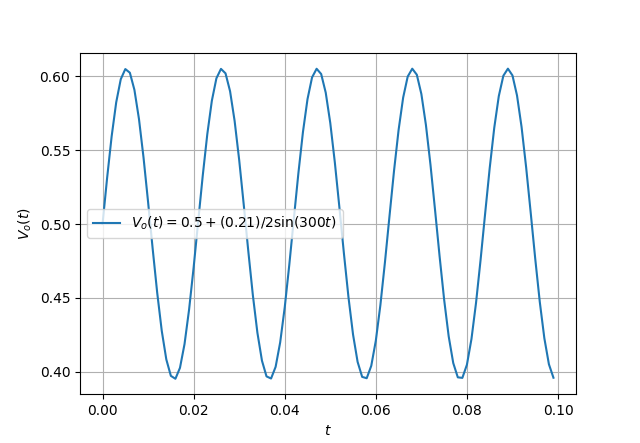
\includegraphics[width=\columnwidth]{59/figs/59fig.png}
    \caption{line plot }
    \label{fig:1}
\end{figure}
\end{document}


\pagebreak

\item The R-L circuit with $R=10 k\Omega$ and $L=1 mH$ is excited by a step current $I_0u(t)$. At $t=0^-$, there is a current $I_L=I_0/5$ flowing through the inductor. The minimum time taken for the current through the inductor to reach $99\%$ of its final value is $\ldots \mu s$
(rounded off to two decimal places).\\
\hfill{(GATE IN 2023)}
\solution
\iffalse
\let\negmedspace\undefined
\let\negthickspace\undefined
\documentclass[journal,12pt,twocolumn]{IEEEtran}
\usepackage{cite}
\usepackage{amsmath,amssymb,amsfonts,amsthm}
\usepackage{algorithmic}
\usepackage{circuitikz}
\usepackage{graphicx}
\usepackage{textcomp}
\usepackage{xcolor}
\usepackage{txfonts}
\usepackage{listings}
\usepackage{enumitem}
\usepackage{mathtools}
\usepackage{gensymb}
\usepackage{comment}
\usepackage[breaklinks=true]{hyperref}
\usepackage{tkz-euclide} 
\usepackage{listings}
\usepackage{gvv}                                        
\def\inputGnumericTable{}                                 
\usepackage[latin1]{inputenc}                                
\usepackage{color}                                            
\usepackage{array}                                            
\usepackage{longtable}                                       
\usepackage{calc}                                             
\usepackage{multirow}                                         
\usepackage{hhline}                                           
\usepackage{ifthen}                                           
\usepackage{lscape}
\newtheorem{theorem}{Theorem}[section]
\newtheorem{problem}{Problem}
\newtheorem{proposition}{Proposition}[section]
\newtheorem{lemma}{Lemma}[section]
\newtheorem{corollary}[theorem]{Corollary}
\newtheorem{example}{Example}[section]
\newtheorem{definition}[problem]{Definition}
\newcommand{\BEQA}{\begin{eqnarray}}
\newcommand{\EEQA}{\end{eqnarray}}
\newcommand{\define}{\stackrel{\triangle}{=}}
\theoremstyle{remark}
\newtheorem{rem}{Remark}
\begin{document}

\bibliographystyle{IEEEtran}
\vspace{3cm}
\title{NCERT Question 11.9.3.9}
\author{EE23BTECH11019 - Faisal Imtiyaz $^{*}$% <-this % stops a space
}
\maketitle
\newpage
\bigskip

\renewcommand{\thefigure}{\arabic{figure}}
\renewcommand{\thetable}{\arabic{table}}


\vspace{3cm}
\textbf{Question:}
The R-L circuit with $R=10 k\Omega$ and $L=1 mH$ is excited by a step current $I_0u(t)$. At $t=0^-$, there is a current $I_L=I_0/5$ flowing through the inductor. The minimum time taken for the current through the inductor to reach $99\%$ of its final value is $\ldots \mu s$
(rounded off to two decimal places).\\
\begin{figure}[h!]
    \centering
    \includegraphics[width=0.8\columnwidth]{question.png}
\end{figure}
\textbf{Solution:}\\
\fi
\begin{tikzpicture}[american]
    % Draw components
    \draw (0,0) to[american current source, l=$I_0$] (0,3); % Current source
    \draw (0,3) -- (2,3) to[R, l=$R$, i=$I_R$] (2,0); % Resistor
    \draw (2,3) -- (4,3) to[L, l=$L$, i=$I_L$] (4,0); % Inductor
    \draw (4,0) -- (0,0); % Connection between resistor and inductor
\end{tikzpicture}

\begin{table}[htbp]
    \centering
    \def\arraystretch{1.5}
    \begin{tabular}{|p{2.5cm}|p{3cm}|}
        \hline
        \textbf{Transform} & \textbf{Signal} \\
        \hline
        $\frac{1}{s(s+a)}$ & $\frac{1}{a}(1-e^{-at})$ \\
        \hline
        $\frac{1}{s+a}$ & $e^{-at}$ \\
        \hline
    \end{tabular}
    \caption{Inverse Laplace transform pairs}
    \label{laplace-transform-pairs-table}
\end{table}

\begin{align}
    I_0u\brak{t} &= I_R + I_L
\end{align}
From KVL, we have:
\begin{align}
    (\frac{I_0}{s} -I_L\brak{s})R - L(sI_L\brak{s} - I_L\brak{0^-}) &=0
\end{align}
After Simplyfying we have:
\begin{align}
    I_L\brak{s} &= \frac{ I_0R +LsI_L\brak{0^-}}{s(R+Ls)}\\
    I_L\brak{s} &= \frac{I_0R}{L}\frac{1}{s(s+\frac{R}{L})} + \frac{I_0}{5}\frac{1}{\frac{R}{L}+s}
\end{align}
From \tabref{laplace-transform-pairs-table}, we have:
\begin{align}
    I_L\brak{t} & = \frac{I_0R}{L} \sbrak{\frac{1}{\frac{R}{L}}(1-e^{-\frac{R}{L}t})} + \frac{I_0}{5}e^{-\frac{R}{L}}\\
    I_L\brak{t} &= I_0 -\frac{4}{5}I_0e^{-\frac{R}{L}t}\\
    I_L\brak{t} &= I_0 -\frac{4}{5}I_0e^{-10^{7}t}\\
    \lim_{t \to \infty} I_L\brak{t} &= I_0
\end{align}
Now time when current in inductor is $99\%$ of its final value is given by:
\begin{align}
    0.99I_0 &= I_0 -\frac{4}{5}I_0e^{-\frac{R}{L}t}\\
    0.01I_0 &= \frac{4}{5}I_0e^{-\frac{R}{L}t}\\
    t &= \frac{L}{R}\ln(80)\\
    t &= 10^{-7}\ln(80) \mu s\\
    t &= 0.43 \mu s
\end{align}
\begin{figure}[ht!]
	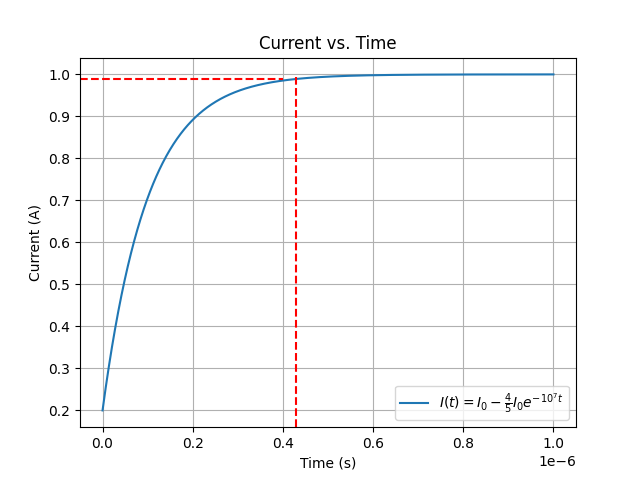
\includegraphics[width=\columnwidth]{2023/IN/47/plots/Figure_1.png}
	% \caption{Plot of $y(n)$ for $a=0.7$}
\end{figure}

  
% \end{document}
\pagebreak


\end{enumerate}

\chapter{ Z-transform}
\chapter{Systems}
\begin{enumerate}[label=\thechapter.\arabic*,ref=\thechapter.\theenumi]

\item Consider a unity-gain negative feedback system consisting of the plant $G\brak{s}$  and a proportional-integral controller. Let the proportional gain and integral
gain be 3 and 1, respectively. For a unit step reference input, the final values of the
controller output and the plant output, respectively, are
\begin{align}
    G\brak{s} = \frac{1}{\brak{s-1}} \notag
\end{align}\hfill (GATE EE 2023)\\
\solution 
\iffalse
\let\negmedspace\undefined
\let\negthickspace\undefined
\documentclass[journal,12pt,twocolumn]{IEEEtran}
\usepackage{cite}
\usepackage{amsmath,amssymb,amsfonts}
\usepackage{graphicx}
\usepackage{textcomp}
\usepackage{xcolor}
\usepackage{txfonts}
\usepackage{listings}
\usepackage{enumitem}
\usepackage{mathtools}
\usepackage{gensymb}
\usepackage{comment}
\usepackage[breaklinks=true]{hyperref}
\usepackage{tkz-euclide} 
\usepackage{listings}
\usepackage{gvv}                                        
\def\inputGnumericTable{}                                 
\usepackage[latin1]{inputenc}                                
\usepackage{color}                                            
\usepackage{array}                                            
\usepackage{longtable}                                       
\usepackage{calc}                                             
\usepackage{multirow}                                         
\usepackage{hhline}                                           
\usepackage{ifthen}                                           
\usepackage{lscape}
\usepackage[export]{adjustbox}

\newtheorem{theorem}{Theorem}[section]
\newtheorem{problem}{Problem}
\newtheorem{proposition}{Proposition}[section]
\newtheorem{lemma}{Lemma}[section]
\newtheorem{corollary}[theorem]{Corollary}
\newtheorem{example}{Example}[section]
\newtheorem{definition}[problem]{Definition}
\newcommand{\BEQA}{\begin{eqnarray}}
\newcommand{\EEQA}{\end{eqnarray}}
\newcommand{\define}{\stackrel{\triangle}{=}}
\newtheorem{rem}{Remark}

\begin{document}
\parindent 0px
\bibliographystyle{IEEEtran}

\vspace{3cm}

\title{}
\author{EE23BTECH11042 -  Khusinadha Naik$^{*}$
}
\maketitle
\newpage
\bigskip

% \renewcommand{\thefigure}{\theenumi}
% \renewcommand{\thetable}{\theenumi}


\noindent \textbf{26.} \hspace{2pt}A causal, discrete time system is described by the difference equation $y[n] = 0.5 y[n-1] + x[n]$, for all $n$, where $y[n]$ denotes the output sequence and $x[n]$ denotes the input sequence. Which of the following statements is/are TRUE?
\begin{flushright}
\hfill(GATE 2023 BM)
\end{flushright}
\begin{enumerate}[label = (\alph*)]
	\item The system has an impulse response described by $0.5^{n} u[-n]$ where $u[n]$ is the  
unit step sequence. 	\label{option:GATE.2023.BM.26.1}	
	\item The system is stable in the bounded input, bounded output sense.		\label{option:GATE.2023.BM.26.2}
	\item The system has an infinite number of non-zero samples in its impulse response	\label{option:GATE.2023.BM.26.3}
	\item The system has a finite number of non-zero samples in its impulse response.	\label{option:GATE.2023.BM.26.4}
\end{enumerate}

\noindent \textbf{Ans.}\\
\fi
\begin{table}[h]
\centering
\begin{tabular}{|c|c|c|}
        \hline
        \textbf{Parameter} & \textbf{Value} & \textbf{Description} \\
        \hline
        $x[n]$ & ? & Input Sequence \\
        \hline
        $y[n]$ & ? & Output Sequence \\
        \hline
\end{tabular}
\caption{Input parameters table}
\label{tab:GATE.2023.BM.26.1}





\end{table}
\begin{align}
y[n] = 0.5y[n-1] + x[n] 
\end{align}

Taking $Z$-Transform 
\begin{align}
Y\brak{z} &= 0.5z^{-1}Y\brak{z} + X\brak{z} \\
\implies \frac{Y\brak{z}}{X\brak{z}} &= \frac{1}{1 - 0.5z^{-1}} = H\brak{z} 
\end{align}
If $x[n]$ is impulse input 
\begin{align}
\implies &Y\brak{z} = H\brak{z} = \frac{1}{1 - 0.5z^{-1}}  \label{eq:GATE.2023.BM.26.4}
\end{align}
From \eqref{eq:GATE.2023.BM.26.4} pole lies at $z = 0.5$
\begin{align}
a^{n}u\brak{n} \xleftrightarrow{\mathcal{Z}} &\frac{1}{1 - az^{-1}} \quad , \abs{z} > a \label{eq:GATE.2023.BM.26.5}
\end{align}

From \eqref{eq:GATE.2023.BM.26.4} , \eqref{eq:GATE.2023.BM.26.5}
\begin{align}
h[n] = 0.5^{n}u[n] \quad , \abs{z} > 0.5 \label{eq:GATE.2023.BM.26.6}
\end{align}


\pagebreak
Plotting $h[n]$ vs $n$
\begin{figure}[h]
    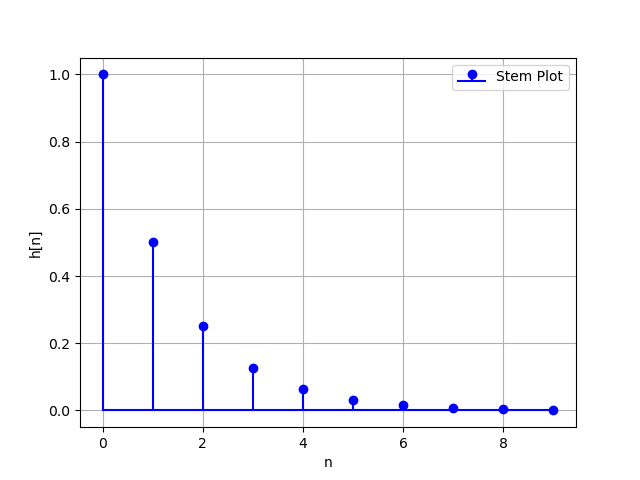
\includegraphics[width=0.5\textwidth]{2023/BM/26/figs/fig1.png}
    \caption{Plot of $h[n]$ vs $n$}
    \label{fig:GATE.2023.BM.26.1}
\end{figure}

\begin{enumerate}
\item From \eqref{eq:GATE.2023.BM.26.6} , \ref{option:GATE.2023.BM.26.1} is wrong
\item As pole lies within unit circle \ref{option:GATE.2023.BM.26.2} is true
\item From \eqref{eq:GATE.2023.BM.26.6} and \figref{fig:GATE.2023.BM.26.1} ,\ref{option:GATE.2023.BM.26.3} is true and hence
\item \ref{option:GATE.2023.BM.26.4} is false 
\end{enumerate}





%\end{document}

\newpage

\item Level \brak{h} in a steam boiler is controlled by manipulating the flow rate \brak{F} of the break-up(fresh) water using a proportional \brak{P} controller. The transfer function between the output and the manipulated input is   \\
$$ \frac{h\brak{s}}{F\brak{s}}=\frac{0.25\brak{1-s}}{s\brak{2s+1}} $$   \\
The measurement and the valve transfer functions are both equal to 1. A process engineer wants to tune the controller so that the closed loop response gives the decaying oscillations under the servo mode. Which one of the following is the CORRECT value of the controller gain to be used by the engineer? \\
\begin{enumerate}[label=(\alph*)]
    \item $0.25$
    \item $2$
    \item $4$
    \item $6$
\end{enumerate} \hfill{GATE CH 2023} \\

\solution
\documentclass[journal,12pt,twocolumn]{IEEEtran}

% Packages
\usepackage{cite}
\usepackage{amsmath,amssymb,amsfonts,amsthm}
\usepackage{graphicx}
\usepackage{textcomp}
\usepackage{xcolor}
\usepackage{txfonts}
\usepackage{listings}
\usepackage{enumitem}
\usepackage{mathtools}
\usepackage{float}
\usepackage{gensymb}
\usepackage{comment}
\usepackage{hyperref}
\usepackage{tkz-euclide}
\usepackage{gvv}
\usepackage[latin1]{inputenc}
\usepackage{color}
\usepackage{array}
\usepackage{longtable}
\usepackage{calc}
\usepackage{multirow}
\usepackage{hhline}
\usepackage{ifthen}
\usepackage{lscape}
\usepackage{subcaption}
\usepackage{tikz}
\usepackage{circuitikz}
\usepackage{wrapfig}
\usepackage{lipsum}
\usepackage[export]{adjustbox}
\usepackage{inputenc}

% Custom commands and macros
\newtheorem{theorem}{Theorem}[section]
\newtheorem{problem}{Problem}
\newtheorem{proposition}{Proposition}[section]
\newtheorem{lemma}{Lemma}[section]
\newtheorem{corollary}[theorem]{Corollary}
\newtheorem{example}{Example}[section]
\newtheorem{definition}[problem]{Definition}
\newtheorem{rem}{Remark}
\newcommand{\BEQA}{\begin{eqnarray}}
\newcommand{\EEQA}{\end{eqnarray}}
\newcommand{\define}{\stackrel{\triangle}{=}}
\renewcommand{\thefigure}{\theenumi}
\renewcommand{\thetable}{\theenumi}



\begin{document}

\title{GATE 2023 EC 49}
\author{EE23BTECH11045 - Palavelli Srija$^{*}$}
\maketitle

\bigskip

\textbf{Question 12.7.7:} 
Let $x(t) = 10 \cos(10.5 \omega t)$ be passed through an LTI system with impulse response $h(t) = \pi\left(\frac{\sin(\omega t)}{\pi t}\right)^2 \cos(10 \omega t)$ . The output of the system is: \\

\textbf{Solution:}
\begin{table}[h!]
    \centering
    \begin{table}[htbp]
	\centering
	\noindent
	\fontsize{10}{15}\selectfont {
		\resizebox{0.45\textwidth}{!}{%
			\begin{tabular}{|c|c|c|}
				\hline
				\textbf{Parameter} & \textbf{Value} & \textbf{Description} \\
				\hline
				$x\brak t$ & - & Input voltage \\
				\hline
				$y\brak t$ & - & Output voltage \\
				\hline
				$h\brak t$ & $\frac{y\brak t}{x\brak t}$ & Impulse response \\
				\hline
				$X\brak s$ & - & Input voltage in s-domain \\
				\hline
				$Y\brak s$ & - & Output voltage in s-domain \\
				\hline
				$H\brak s$ & $\frac{Y\brak s}{X\brak s}$ & Impulse response in s-domain \\
				\hline
			\end{tabular}
	} }
	\caption*{Input Table}
	
\end{table}
    \caption{Input Parameters}
    \label{tab:table_sr10}
\end{table}

Given \(h(t)\) is real and even. When a sinusoidal input is applied to an LTI system with an even impulse response, the output will also be sinusoidal. Hence, \(y(t) = A\cdot 10\cos(10.5 \omega t + \theta)\).

\[
x(t) \xrightarrow{\text{}} \boxed{\text{h(t)}} \xrightarrow{\text{}} y(t)
\]

\begin{align}
\text{Let } f(t) &= \pi\left(\frac{\sin(\omega t)}{\pi t}\right)^2 \\
h(t) &= f(t) \cos(10 \omega t)
\end{align}

Using 
\begin{align}
x_1(t) \cdot x_2(t) \xleftrightarrow{\mathcal{F}} X_1(\omega) * X_2(\omega)\\
\left(\frac{\sin(\omega t)}{\pi t}\right) \cdot \left(\frac{\sin(\omega t)}{\pi t}\right) \xleftrightarrow{\mathcal{F}} X_1(\omega) * X_2(\omega)
\end{align}
\begin{figure}[h!]
    \centering
    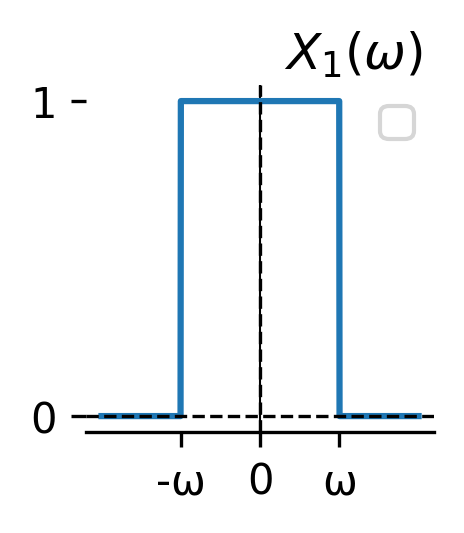
\includegraphics[width=0.4\columnwidth, height=2.5cm]{figs/plot.png}\hfill
    \begin{tabular}{c}
        {\sffamily\raisebox{1.75cm}{*}} 
    \end{tabular}\hfill
    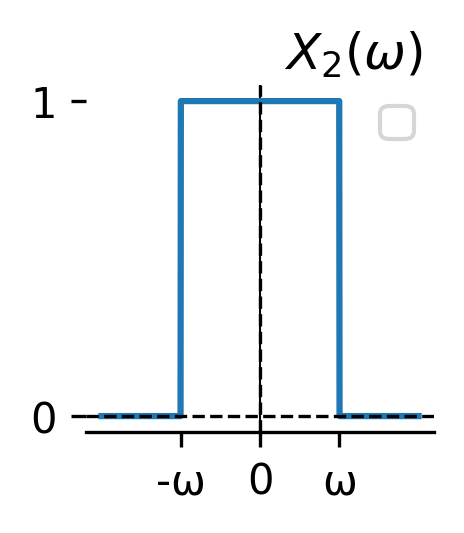
\includegraphics[width=0.4\columnwidth, height=2.5cm]{figs/plot4.png}
    
    \caption{}
    \label{fig:overall}
\end{figure}

\begin{align}
\left(\frac{\sin(\omega t)}{\pi t}\right)^2  \xleftrightarrow{\mathcal{F}} X_3(\omega) 
\end{align}
\begin{figure}[h!]
    \centering
    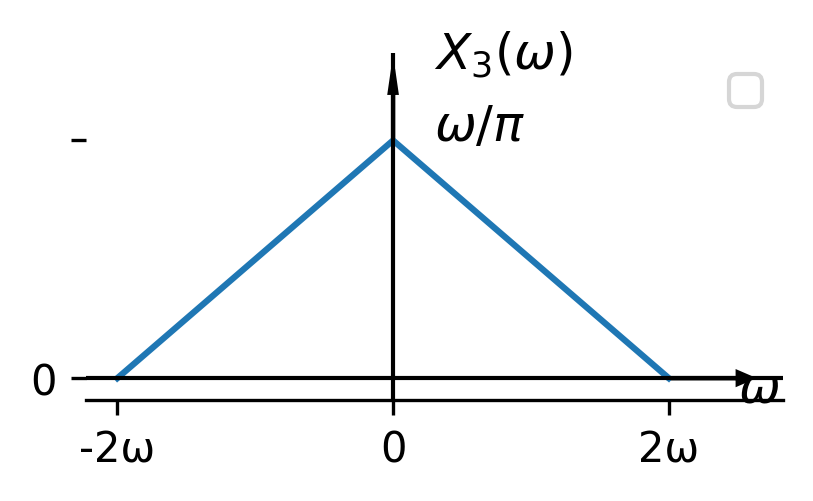
\includegraphics[width=0.5\columnwidth, height=3cm]{figs/plot1.png}
    \caption{}
    \label{fig:sr11}
\end{figure}
\begin{align}
\pi\left(\frac{\sin(\omega t)}{\pi t}\right)^2 \xleftrightarrow{\mathcal{F}} X_4(\omega)
\end{align}
\begin{figure}[h!]
    \centering
    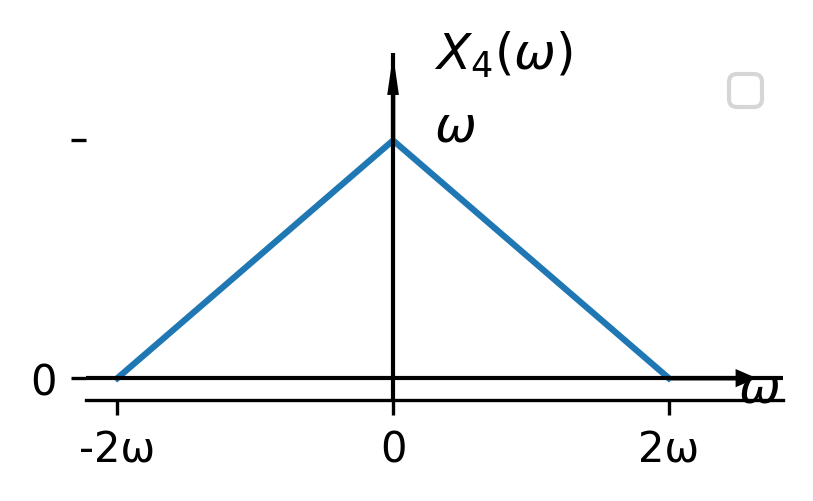
\includegraphics[width=0.5\columnwidth, height=3cm]{figs/plot2.png}
    \caption{}
    \label{fig:sr12}
\end{figure}
    \begin{align}
\text{From modulating property:} \nonumber \\
        f(t) \cos(\omega_0 t) \xleftrightarrow{\mathcal{F}} \frac{1}{2} \left[F(\omega + \omega_0) + F(\omega - \omega_0)\right]
    \end{align}

    \begin{align}
        H(\omega) &= \frac{1}{2} \left[F(\omega + 10\omega) + F(\omega - 10\omega)\right]
    \end{align}

\begin{figure}[h!]
    \centering
    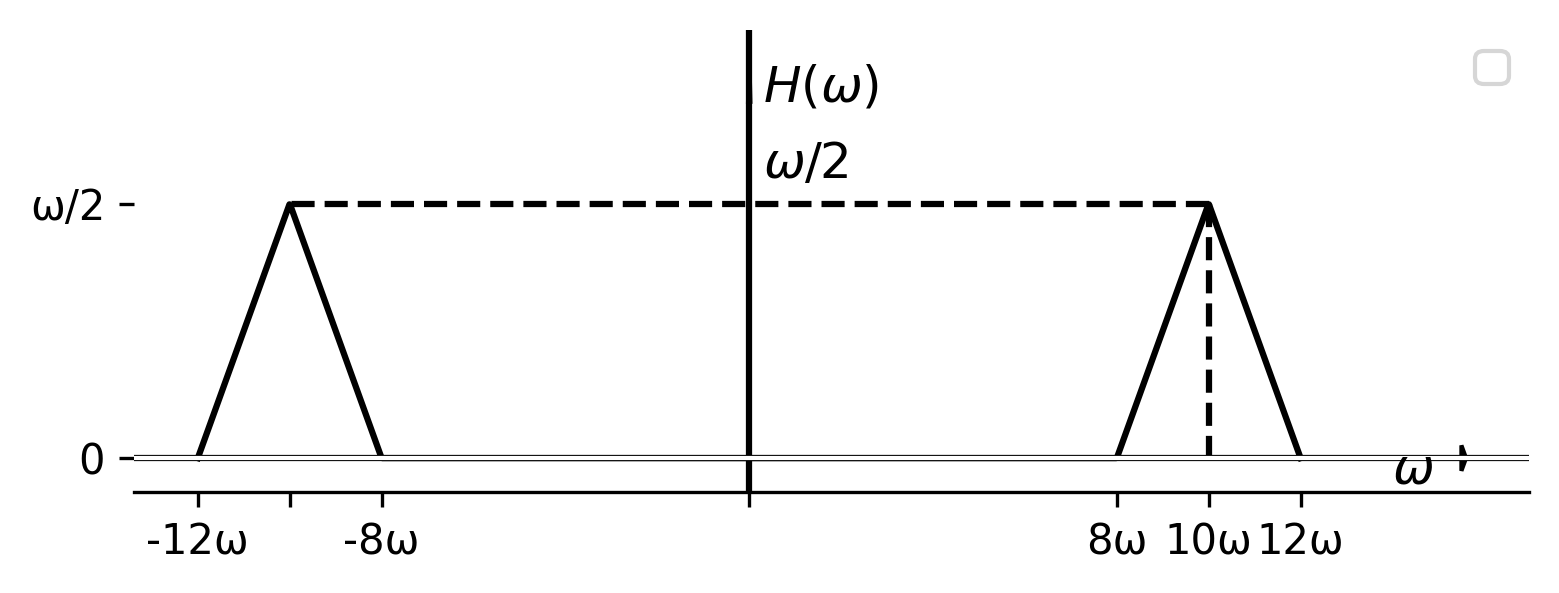
\includegraphics[width=0.7\columnwidth,height=2.5cm]{figs/plot3.png}
    \caption{}
    \label{fig:sr13}
\end{figure}
\begin{equation}
    \frac{\frac{\omega}{2} - 0}{10\omega - 12\omega} = \frac{|H(10.5\omega)| - 0}{10.5\omega - 12\omega}
\end{equation}

\begin{align}
A = |H(10.5\omega)| &= \frac{3}{8}\omega \quad \text{and} \quad  \theta= \angle H(10.5\omega) = 0^\circ
\end{align}

The output \(y(t)\):
\begin{align}
y(t) &= \frac{3}{8}\omega \cdot 10 \cos(10.5 \omega t) \\
&= \frac{15}{4}\omega \cos(10.5 \omega t)
\end{align}
\begin{figure}[h!]
    \centering
    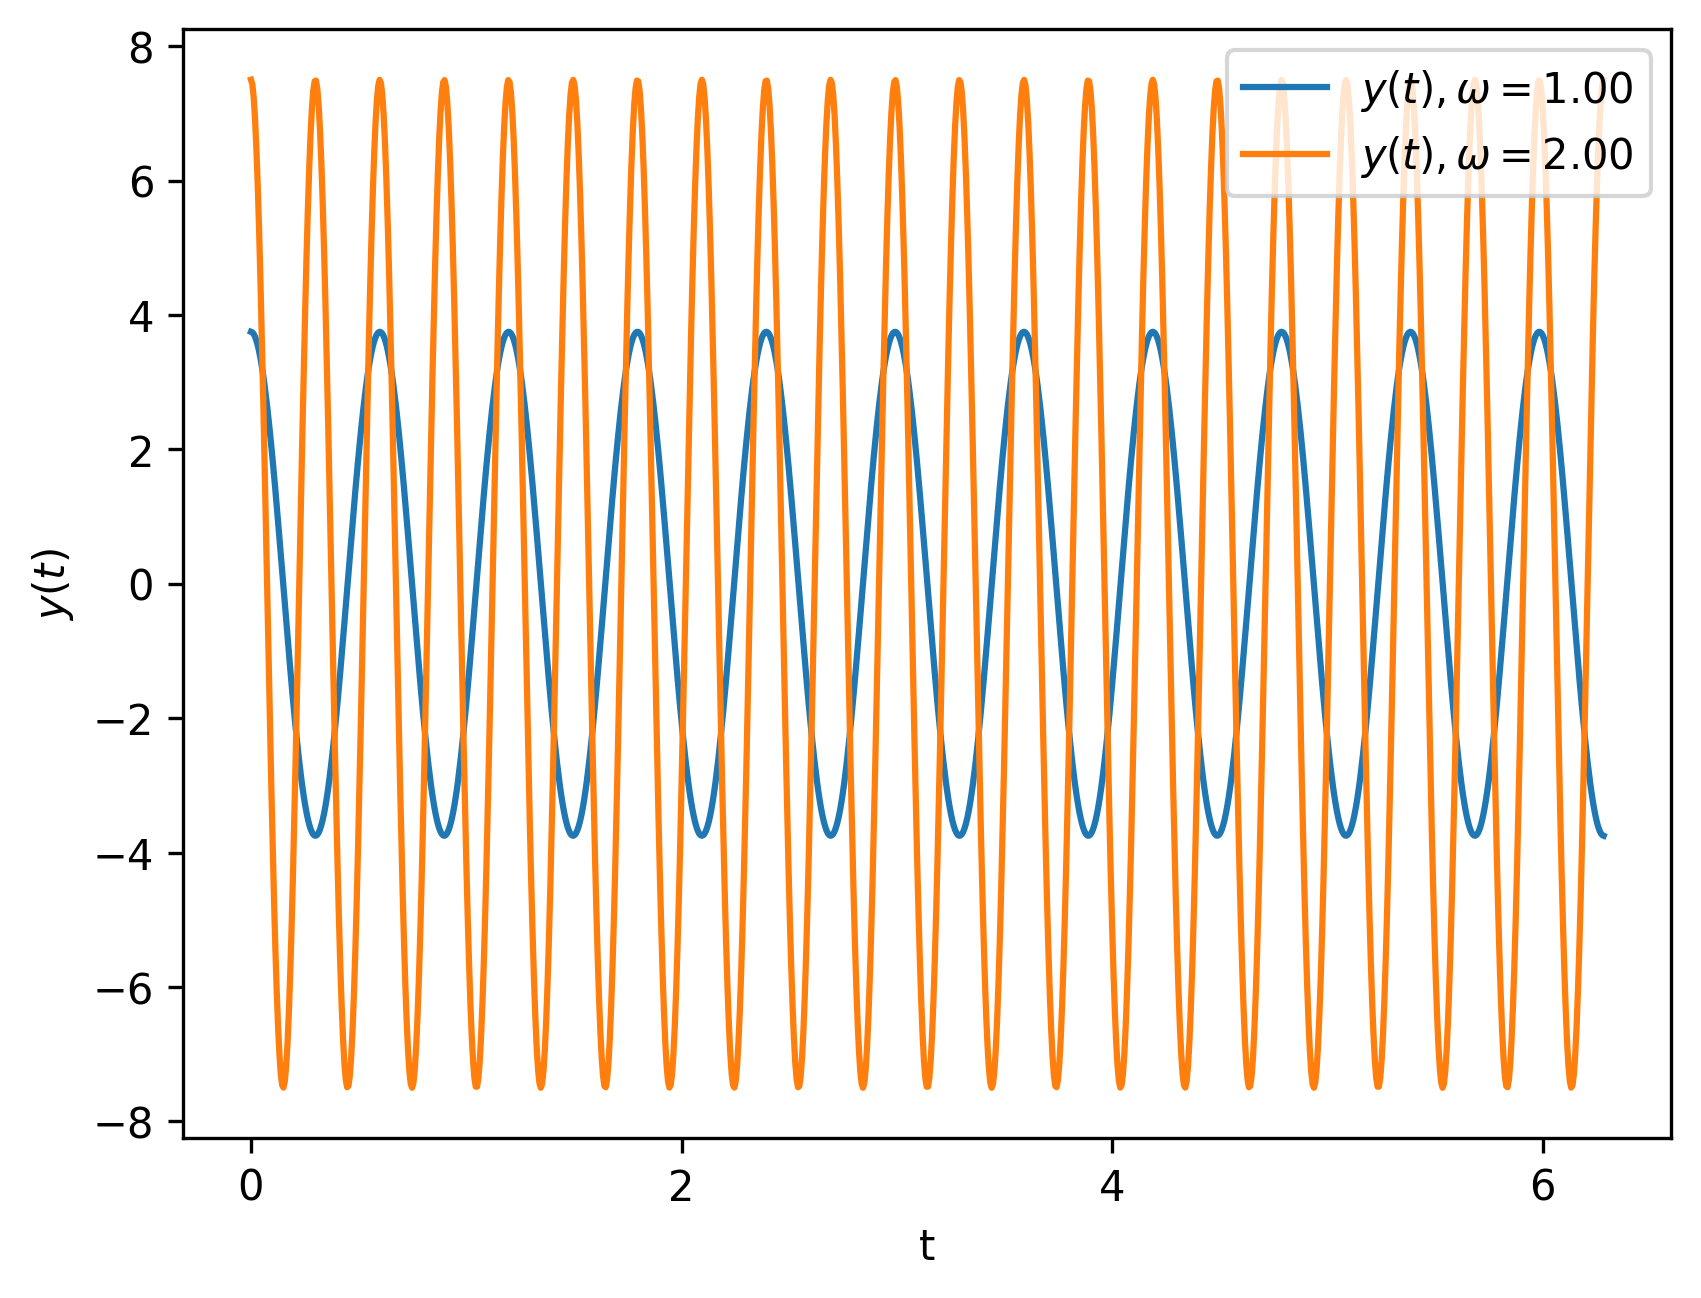
\includegraphics[width=\columnwidth]{figs/plot5.png}
    \caption{}
    \label{fig:sr14}
\end{figure}
\end{document}


\newpage
\item The figure shows a block of mass m = 20 kg attached to a pair of identical linear springs, each having a spring constant k = 1000 N/m. The block oscillates on a frictionless horizontal surface. Assuming free vibrations, the time taken by the block to complete ten oscillations is \rule{1cm}{0.15mm} seconds . (Rounded off to two decimal places) Take $\pi$ = 3.14. \\ \hfill(GATE ME 2023)

\begin{figure}[!ht]
\centering
\begin{center}
\includegraphics[width=\columnwidth]{2023/ME/30/figs/questiondiagram.jpg}
\end{center}
%\caption{Diagram for GATE ME Question 30}
\end{figure}
\solution
\input{2023/ME/30/me30.tex}
\newpage

\item A system has transfer function
 \[\frac{Y(s)}{X(s)}=\frac {s-\pi}{s+\pi}\]
 let $u(t)$ be the unit step function.The input $x(t)$ that results in a steady-state output $y(t)=sin(\pi t)$ is \underline{\quad}.\hfill (GATE IN 2023)\\
 \solution
 \iffalse
\let\negmedspace\undefined
\let\negthickspace\undefined
\documentclass[journal,12pt,twocolumn]{IEEEtran}
\usepackage{cite}
\usepackage{amsmath,amssymb,amsfonts}
\usepackage{graphicx}
\usepackage{textcomp}
\usepackage{xcolor}
\usepackage{txfonts}
\usepackage{listings}
\usepackage{enumitem}
\usepackage{mathtools}
\usepackage{gensymb}
\usepackage{comment}
\usepackage[breaklinks=true]{hyperref}
\usepackage{tkz-euclide} 
\usepackage{listings}
\usepackage{gvv}                                        
\def\inputGnumericTable{}                                 
\usepackage[latin1]{inputenc}                                
\usepackage{color}                                            
\usepackage{array}                                            
\usepackage{longtable}                                       
\usepackage{calc}                                             
\usepackage{multirow}                                         
\usepackage{hhline}                                           
\usepackage{ifthen}                                           
\usepackage{lscape}
\usepackage[export]{adjustbox}

\newtheorem{theorem}{Theorem}[section]
\newtheorem{problem}{Problem}
\newtheorem{proposition}{Proposition}[section]
\newtheorem{lemma}{Lemma}[section]
\newtheorem{corollary}[theorem]{Corollary}
\newtheorem{example}{Example}[section]
\newtheorem{definition}[problem]{Definition}
\newcommand{\BEQA}{\begin{eqnarray}}
\newcommand{\EEQA}{\end{eqnarray}}
\newcommand{\define}{\stackrel{\triangle}{=}}
\newtheorem{rem}{Remark}

\begin{document}
\parindent 0px
\bibliographystyle{IEEEtran}

\vspace{3cm}

\title{}
\author{EE23BTECH11042 -  Khusinadha Naik$^{*}$
}
\maketitle
\newpage
\bigskip

% \renewcommand{\thefigure}{\theenumi}
% \renewcommand{\thetable}{\theenumi}


\noindent \textbf{26.} \hspace{2pt}A causal, discrete time system is described by the difference equation $y[n] = 0.5 y[n-1] + x[n]$, for all $n$, where $y[n]$ denotes the output sequence and $x[n]$ denotes the input sequence. Which of the following statements is/are TRUE?
\begin{flushright}
\hfill(GATE 2023 BM)
\end{flushright}
\begin{enumerate}[label = (\alph*)]
	\item The system has an impulse response described by $0.5^{n} u[-n]$ where $u[n]$ is the  
unit step sequence. 	\label{option:GATE.2023.BM.26.1}	
	\item The system is stable in the bounded input, bounded output sense.		\label{option:GATE.2023.BM.26.2}
	\item The system has an infinite number of non-zero samples in its impulse response	\label{option:GATE.2023.BM.26.3}
	\item The system has a finite number of non-zero samples in its impulse response.	\label{option:GATE.2023.BM.26.4}
\end{enumerate}

\noindent \textbf{Ans.}\\
\fi
\begin{table}[h]
\centering
\begin{tabular}{|c|c|c|}
        \hline
        \textbf{Parameter} & \textbf{Value} & \textbf{Description} \\
        \hline
        $x[n]$ & ? & Input Sequence \\
        \hline
        $y[n]$ & ? & Output Sequence \\
        \hline
\end{tabular}
\caption{Input parameters table}
\label{tab:GATE.2023.BM.26.1}





\end{table}
\begin{align}
y[n] = 0.5y[n-1] + x[n] 
\end{align}

Taking $Z$-Transform 
\begin{align}
Y\brak{z} &= 0.5z^{-1}Y\brak{z} + X\brak{z} \\
\implies \frac{Y\brak{z}}{X\brak{z}} &= \frac{1}{1 - 0.5z^{-1}} = H\brak{z} 
\end{align}
If $x[n]$ is impulse input 
\begin{align}
\implies &Y\brak{z} = H\brak{z} = \frac{1}{1 - 0.5z^{-1}}  \label{eq:GATE.2023.BM.26.4}
\end{align}
From \eqref{eq:GATE.2023.BM.26.4} pole lies at $z = 0.5$
\begin{align}
a^{n}u\brak{n} \xleftrightarrow{\mathcal{Z}} &\frac{1}{1 - az^{-1}} \quad , \abs{z} > a \label{eq:GATE.2023.BM.26.5}
\end{align}

From \eqref{eq:GATE.2023.BM.26.4} , \eqref{eq:GATE.2023.BM.26.5}
\begin{align}
h[n] = 0.5^{n}u[n] \quad , \abs{z} > 0.5 \label{eq:GATE.2023.BM.26.6}
\end{align}


\pagebreak
Plotting $h[n]$ vs $n$
\begin{figure}[h]
    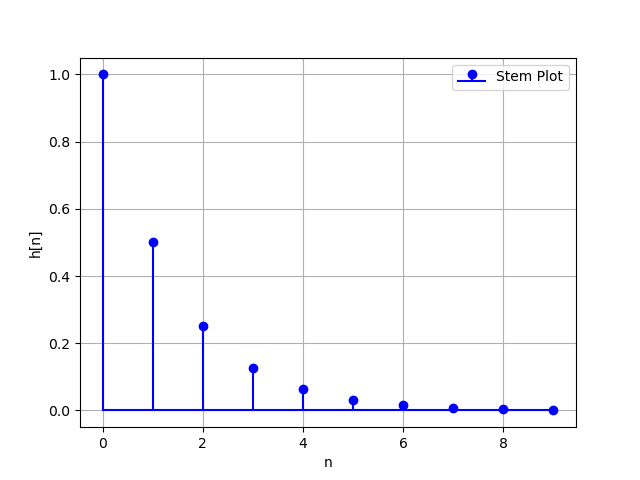
\includegraphics[width=0.5\textwidth]{2023/BM/26/figs/fig1.png}
    \caption{Plot of $h[n]$ vs $n$}
    \label{fig:GATE.2023.BM.26.1}
\end{figure}

\begin{enumerate}
\item From \eqref{eq:GATE.2023.BM.26.6} , \ref{option:GATE.2023.BM.26.1} is wrong
\item As pole lies within unit circle \ref{option:GATE.2023.BM.26.2} is true
\item From \eqref{eq:GATE.2023.BM.26.6} and \figref{fig:GATE.2023.BM.26.1} ,\ref{option:GATE.2023.BM.26.3} is true and hence
\item \ref{option:GATE.2023.BM.26.4} is false 
\end{enumerate}





%\end{document}

 \newpage

\item Consider the complex function
\[ f(z) = \frac{z^{2}\sin z}{(z-\pi)^4} \]
At \( z = \pi \), which of the following options is (are) correct?
\begin{enumerate}[label=\textbf{\arabic*.}, font=\bfseries, align=left]
    \item[(A)] The order of the pole is 4 
    \item[(B)] The order of the pole is 3 
    \item[(C)] The residue at the pole is \( \frac{\pi}{6} \)
    \item[(D)] The residue at the pole is \( \frac{2\pi}{3} \)
\end{enumerate}
\hfill (GATE PH 2023)
\solution
\iffalse
\let\negmedspace\undefined
\let\negthickspace\undefined
\documentclass[journal,12pt,onecolumn]{IEEEtran}
\usepackage{cite}
\usepackage{amsmath,amssymb,amsfonts,amsthm}

\usepackage{graphicx}
\usepackage{textcomp}
\usepackage{xcolor}
\usepackage{txfonts}
\usepackage{listings}
\usepackage{enumitem}
\usepackage{mathtools}
\usepackage{gensymb}
\usepackage[breaklinks=true]{hyperref}
\usepackage{tkz-euclide} % loads  TikZ and tkz-base
\usepackage{listings}
\usepackage{gvv}
\usepackage{booktabs}

%
%\usepackage{setspace}
%\usepackage{gensymb}
%\doublespacing
%\singlespacing

%\usepackage{graphicx}
%\usepackage{amssymb}
%\usepackage{relsize}
%\usepackage[cmex10]{amsmath}
%\usepackage{amsthm}
%\interdisplaylinepenalty=2500
%\savesymbol{iint}
%\usepackage{txfonts}
%\restoresymbol{TXF}{iint}
%\usepackage{wasysym}
%\usepackage{amsthm}
%\usepackage{iithtlc}
%\usepackage{mathrsfs}
%\usepackage{txfonts}
%\usepackage{stfloats}
%\usepackage{bm}
%\usepackage{cite}
%\usepackage{cases}
%\usepackage{subfig}
%\usepackage{xtab}
%\usepackage{longtable}
%\usepackage{multirow}

%\usepackage{algpseudocode}
%\usepackage{enumitem}
%\usepackage{mathtools}
%\usepackage{tikz}
%\usepackage{circuitikz}
%\usepackage{verbatim}
%\usepackage{tfrupee}
%\usepackage{stmaryrd}
%\usetkzobj{all}
%    \usepackage{color}                                            %%
%    \usepackage{array}                                            %%
%    \usepackage{longtable}                                        %%
%    \usepackage{calc}                                             %%
%    \usepackage{multirow}                                         %%
%    \usepackage{hhline}                                           %%
%    \usepackage{ifthen}                                           %%
  %optionally (for landscape tables embedded in another document): %%
%    \usepackage{lscape}     
%\usepackage{multicol}
%\usepackage{chngcntr}
%\usepackage{enumerate}

%\usepackage{wasysym}
%\documentclass[conference]{IEEEtran}
%\IEEEoverridecommandlockouts
% The preceding line is only needed to identify funding in the first footnote. If that is unneeded, please comment it out.

\newtheorem{theorem}{Theorem}[section]
\newtheorem{problem}{Problem}
\newtheorem{proposition}{Proposition}[section]
\newtheorem{lemma}{Lemma}[section]
\newtheorem{corollary}[theorem]{Corollary}
\newtheorem{example}{Example}[section]
\newtheorem{definition}[problem]{Definition}
%\newtheorem{thm}{Theorem}[section] 
%\newtheorem{defn}[thm]{Definition}
%\newtheorem{algorithm}{Algorithm}[section]
%\newtheorem{cor}{Corollary}
\newcommand{\BEQA}{\begin{eqnarray}}
\newcommand{\EEQA}{\end{eqnarray}}
\newcommand{\define}{\stackrel{\triangle}{=}}
\theoremstyle{remark}
\newtheorem{rem}{Remark}

%\bibliographystyle{ieeetr}
\begin{document}
%

\bibliographystyle{IEEEtran}


\vspace{3cm}

\title{
%	\logo{
Gate Question

\large{EE:1205 Signals and Systems}

Indian Institute of Technology, Hyderabad
%	}
}
\author{Abhey Garg

EE23BTECH11202
}	


% make the title area
\maketitle


%\tableofcontents

\bigskip

\renewcommand{\thefigure}{\arabic{figure}}
\renewcommand{\thetable}{\arabic{table}}
\renewcommand{\theequation}{\arabic{equation}}

\section{Question GATE PH 56}
Consider the complex function
\[ f(z) = \frac{z^{2}\sin z}{(z-\pi)^4} \]
At \( z = \pi \), which of the following options is (are) correct?
\begin{enumerate}[label=\textbf{\arabic*.}, font=\bfseries, align=left]
    \item[(A)] The order of the pole is 4 
    \item[(B)] The order of the pole is 3 
    \item[(C)] The residue at the pole is \( \frac{\pi}{6} \)
    \item[(D)] The residue at the pole is \( \frac{2\pi}{3} \)
\end{enumerate}
\hfill (GATE PH 2023)
\section{Solution}
\fi
\begin{table}[ht]
\centering
\setlength{\extrarowheight}{8pt}
\caption{Input Parameters}
\begin{tabular}{|c|l|l|} 
\hline
\textbf{Parameter} & \textbf{Used to denote} & \textbf{Values} \\
\hline
$m$ & order of pole at z = $\pi$  & \multicolumn{1}{|p{1.3cm}|}{\centering $?$ }\\
\hline
$Res(f,\pi)$ & Residue of pole  & \multicolumn{1}{|p{1.3cm}|}{\centering $?$ }\\
\hline
\end{tabular}
 \vspace{4mm}
 \label{tab:cappy}
\end{table}

\begin{enumerate}[label=\textbf{\arabic*.}, font=\bfseries, align=left]
\item[(a)]
As the power of $(z-\pi) $ in denominator is 4 , so the order of the pole is 4.
\item[(b)]
\begin{align}
\text{Res}(f, \pi) &= \frac{1}{(m-1)!} \frac{d^{m-1}}{dz^{m-1}} \left[ (z-\pi)^m f(z) \right] \Bigg|_{z=\pi} \\
\text{Res}(f,\pi) &= \frac{1}{3!} \frac{d^3}{dz^3} \left[ (z-\pi)^4 \frac{z^2 \sin z}{(z-\pi)^4} \right] \Bigg|_{z=\pi} \\
\text{Res}(f,\pi) &= \frac{1}{3!} \frac{d^3}{dz^3} z^2 \sin z \Bigg|_{z=\pi} \\
&= \frac{1}{3!} (6\cos z -6z\sin z -z^2 \cos z) \Bigg|_{z=\pi} \\
\end{align}


Since \( \sin(\pi) = 0 \) and \( \cos(\pi) = -1 \), this simplifies to:


\begin{align}
\text{Res}(f,\pi) &= \frac{\pi^2-6}{3!}  = \frac{\pi^2 - 6}{6}
\end{align}
\end{enumerate}
%\end{document}

\newpage
 \item
 A buoy of virtual mass $30$ kg oscillates in a fluid medium as a single degree of
freedom system. If the total damping in the system is set as $188.5$ N-s/m, such
that the oscillation just ceases to occur, then the natural period of the system is
\rule{1cm}{0.15mm} s (round off to one decimal place)
\hfill(GATE MN 2023 question 63)\\
\solution 
\input{2023/NM/63/asnmt4.tex}
\newpage
\item 
Which of the following statement(s) is/are true?
\begin{enumerate}[label=(\alph*)]
	\item If an LTI system is causal, it is stable.
	\item A discrete time LTI system is causal if and only if its response to a step input $u[n]$ is 0 for $n < 0$.
	\item If a discrete time LTI system has an impulse response $h[n]$ of finite duration the system is stable.
	\item If the impulse response $0 < |h[n]| < 1$ for all $n$, then the LTI system is stable.
\end{enumerate}
\hfill (GATE EE 2023 question 27)\\
\solution
\iffalse
\let\negmedspace\undefined
\let\negthickspace\undefined
\documentclass[journal,12pt,twocolumn]{IEEEtran}
\usepackage{cite}
\usepackage{amsmath,amssymb,amsfonts}
\usepackage{graphicx}
\usepackage{textcomp}
\usepackage{xcolor}
\usepackage{txfonts}
\usepackage{listings}
\usepackage{enumitem}
\usepackage{mathtools}
\usepackage{gensymb}
\usepackage{comment}
\usepackage[breaklinks=true]{hyperref}
\usepackage{tkz-euclide} 
\usepackage{listings}
\usepackage{gvv}                                        
\def\inputGnumericTable{}                                 
\usepackage[latin1]{inputenc}                                
\usepackage{color}                                            
\usepackage{array}                                            
\usepackage{longtable}                                       
\usepackage{calc}                                             
\usepackage{multirow}                                         
\usepackage{hhline}                                           
\usepackage{ifthen}                                           
\usepackage{lscape}
\usepackage[export]{adjustbox}

\newtheorem{theorem}{Theorem}[section]
\newtheorem{problem}{Problem}
\newtheorem{proposition}{Proposition}[section]
\newtheorem{lemma}{Lemma}[section]
\newtheorem{corollary}[theorem]{Corollary}
\newtheorem{example}{Example}[section]
\newtheorem{definition}[problem]{Definition}
\newcommand{\BEQA}{\begin{eqnarray}}
\newcommand{\EEQA}{\end{eqnarray}}
\newcommand{\define}{\stackrel{\triangle}{=}}
\newtheorem{rem}{Remark}

\begin{document}
\parindent 0px
\bibliographystyle{IEEEtran}

\vspace{3cm}

\title{}
\author{EE23BTECH11042 -  Khusinadha Naik$^{*}$
}
\maketitle
\newpage
\bigskip

% \renewcommand{\thefigure}{\theenumi}
% \renewcommand{\thetable}{\theenumi}


\noindent \textbf{26.} \hspace{2pt}A causal, discrete time system is described by the difference equation $y[n] = 0.5 y[n-1] + x[n]$, for all $n$, where $y[n]$ denotes the output sequence and $x[n]$ denotes the input sequence. Which of the following statements is/are TRUE?
\begin{flushright}
\hfill(GATE 2023 BM)
\end{flushright}
\begin{enumerate}[label = (\alph*)]
	\item The system has an impulse response described by $0.5^{n} u[-n]$ where $u[n]$ is the  
unit step sequence. 	\label{option:GATE.2023.BM.26.1}	
	\item The system is stable in the bounded input, bounded output sense.		\label{option:GATE.2023.BM.26.2}
	\item The system has an infinite number of non-zero samples in its impulse response	\label{option:GATE.2023.BM.26.3}
	\item The system has a finite number of non-zero samples in its impulse response.	\label{option:GATE.2023.BM.26.4}
\end{enumerate}

\noindent \textbf{Ans.}\\
\fi
\begin{table}[h]
\centering
\begin{tabular}{|c|c|c|}
        \hline
        \textbf{Parameter} & \textbf{Value} & \textbf{Description} \\
        \hline
        $x[n]$ & ? & Input Sequence \\
        \hline
        $y[n]$ & ? & Output Sequence \\
        \hline
\end{tabular}
\caption{Input parameters table}
\label{tab:GATE.2023.BM.26.1}





\end{table}
\begin{align}
y[n] = 0.5y[n-1] + x[n] 
\end{align}

Taking $Z$-Transform 
\begin{align}
Y\brak{z} &= 0.5z^{-1}Y\brak{z} + X\brak{z} \\
\implies \frac{Y\brak{z}}{X\brak{z}} &= \frac{1}{1 - 0.5z^{-1}} = H\brak{z} 
\end{align}
If $x[n]$ is impulse input 
\begin{align}
\implies &Y\brak{z} = H\brak{z} = \frac{1}{1 - 0.5z^{-1}}  \label{eq:GATE.2023.BM.26.4}
\end{align}
From \eqref{eq:GATE.2023.BM.26.4} pole lies at $z = 0.5$
\begin{align}
a^{n}u\brak{n} \xleftrightarrow{\mathcal{Z}} &\frac{1}{1 - az^{-1}} \quad , \abs{z} > a \label{eq:GATE.2023.BM.26.5}
\end{align}

From \eqref{eq:GATE.2023.BM.26.4} , \eqref{eq:GATE.2023.BM.26.5}
\begin{align}
h[n] = 0.5^{n}u[n] \quad , \abs{z} > 0.5 \label{eq:GATE.2023.BM.26.6}
\end{align}


\pagebreak
Plotting $h[n]$ vs $n$
\begin{figure}[h]
    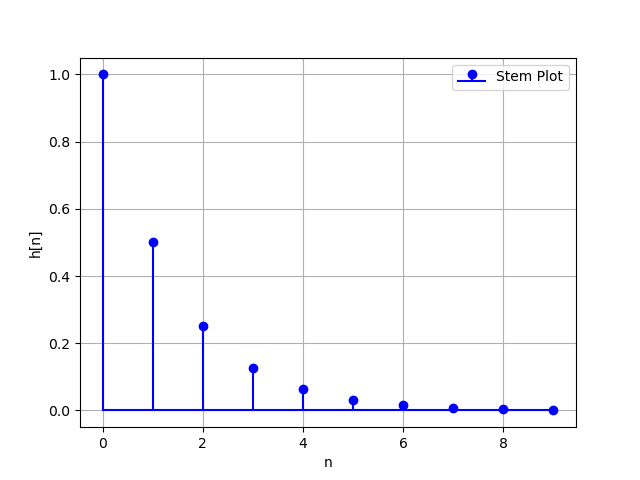
\includegraphics[width=0.5\textwidth]{2023/BM/26/figs/fig1.png}
    \caption{Plot of $h[n]$ vs $n$}
    \label{fig:GATE.2023.BM.26.1}
\end{figure}

\begin{enumerate}
\item From \eqref{eq:GATE.2023.BM.26.6} , \ref{option:GATE.2023.BM.26.1} is wrong
\item As pole lies within unit circle \ref{option:GATE.2023.BM.26.2} is true
\item From \eqref{eq:GATE.2023.BM.26.6} and \figref{fig:GATE.2023.BM.26.1} ,\ref{option:GATE.2023.BM.26.3} is true and hence
\item \ref{option:GATE.2023.BM.26.4} is false 
\end{enumerate}





%\end{document}

\newpage

\item The outlet concentration $C_A$ of a plug flow reactor (PFR) is controlled by manipulating the inlet concentration $C_{A0}$.The following transfer function describes the dynamics of this PFR.
\begin{align*}
    \frac{C_{A}(s)}{C_{A0}(s)}=e^{-(\frac{V}{F})(k+s)}
\end{align*}
In the above question, V=1$m^3$,F=0.1$m^3$$min^{-1}$ and k=0.5$min^{-1}$.The measurement and valve transfer functions are both equal to 1.The ultimate gain, defined as the proportional controller gain that produces sustained oscillations, for this system is\\ \hfill{(GATE 2023 CH 61)}\\
\solution
\item For the block diagram shown in the figure, the transfer function $\frac{Y\brak{s}}{R\brak{s}}$ is \\
\begin{figure}[H]
    {\input{2023/figs/block}}
    \caption{Block diagram}
    \label{fig:gate_ee_Q12_blockdiagram}
\end{figure}
\hfill (GATE EE 2023)\\
\solution
\iffalse
\let\negmedspace\undefined
\let\negthickspace\undefined
\documentclass[journal,12pt,twocolumn]{IEEEtran}
\usepackage{cite}
\usepackage{amsmath,amssymb,amsfonts}
\usepackage{graphicx}
\usepackage{textcomp}
\usepackage{xcolor}
\usepackage{txfonts}
\usepackage{listings}
\usepackage{enumitem}
\usepackage{mathtools}
\usepackage{gensymb}
\usepackage{comment}
\usepackage[breaklinks=true]{hyperref}
\usepackage{tkz-euclide} 
\usepackage{listings}
\usepackage{gvv}                                        
\def\inputGnumericTable{}                                 
\usepackage[latin1]{inputenc}                                
\usepackage{color}                                            
\usepackage{array}                                            
\usepackage{longtable}                                       
\usepackage{calc}                                             
\usepackage{multirow}                                         
\usepackage{hhline}                                           
\usepackage{ifthen}                                           
\usepackage{lscape}
\usepackage[export]{adjustbox}

\newtheorem{theorem}{Theorem}[section]
\newtheorem{problem}{Problem}
\newtheorem{proposition}{Proposition}[section]
\newtheorem{lemma}{Lemma}[section]
\newtheorem{corollary}[theorem]{Corollary}
\newtheorem{example}{Example}[section]
\newtheorem{definition}[problem]{Definition}
\newcommand{\BEQA}{\begin{eqnarray}}
\newcommand{\EEQA}{\end{eqnarray}}
\newcommand{\define}{\stackrel{\triangle}{=}}
\newtheorem{rem}{Remark}

\begin{document}
\parindent 0px
\bibliographystyle{IEEEtran}

\vspace{3cm}

\title{}
\author{EE23BTECH11042 -  Khusinadha Naik$^{*}$
}
\maketitle
\newpage
\bigskip

% \renewcommand{\thefigure}{\theenumi}
% \renewcommand{\thetable}{\theenumi}


\noindent \textbf{26.} \hspace{2pt}A causal, discrete time system is described by the difference equation $y[n] = 0.5 y[n-1] + x[n]$, for all $n$, where $y[n]$ denotes the output sequence and $x[n]$ denotes the input sequence. Which of the following statements is/are TRUE?
\begin{flushright}
\hfill(GATE 2023 BM)
\end{flushright}
\begin{enumerate}[label = (\alph*)]
	\item The system has an impulse response described by $0.5^{n} u[-n]$ where $u[n]$ is the  
unit step sequence. 	\label{option:GATE.2023.BM.26.1}	
	\item The system is stable in the bounded input, bounded output sense.		\label{option:GATE.2023.BM.26.2}
	\item The system has an infinite number of non-zero samples in its impulse response	\label{option:GATE.2023.BM.26.3}
	\item The system has a finite number of non-zero samples in its impulse response.	\label{option:GATE.2023.BM.26.4}
\end{enumerate}

\noindent \textbf{Ans.}\\
\fi
\begin{table}[h]
\centering
\begin{tabular}{|c|c|c|}
        \hline
        \textbf{Parameter} & \textbf{Value} & \textbf{Description} \\
        \hline
        $x[n]$ & ? & Input Sequence \\
        \hline
        $y[n]$ & ? & Output Sequence \\
        \hline
\end{tabular}
\caption{Input parameters table}
\label{tab:GATE.2023.BM.26.1}





\end{table}
\begin{align}
y[n] = 0.5y[n-1] + x[n] 
\end{align}

Taking $Z$-Transform 
\begin{align}
Y\brak{z} &= 0.5z^{-1}Y\brak{z} + X\brak{z} \\
\implies \frac{Y\brak{z}}{X\brak{z}} &= \frac{1}{1 - 0.5z^{-1}} = H\brak{z} 
\end{align}
If $x[n]$ is impulse input 
\begin{align}
\implies &Y\brak{z} = H\brak{z} = \frac{1}{1 - 0.5z^{-1}}  \label{eq:GATE.2023.BM.26.4}
\end{align}
From \eqref{eq:GATE.2023.BM.26.4} pole lies at $z = 0.5$
\begin{align}
a^{n}u\brak{n} \xleftrightarrow{\mathcal{Z}} &\frac{1}{1 - az^{-1}} \quad , \abs{z} > a \label{eq:GATE.2023.BM.26.5}
\end{align}

From \eqref{eq:GATE.2023.BM.26.4} , \eqref{eq:GATE.2023.BM.26.5}
\begin{align}
h[n] = 0.5^{n}u[n] \quad , \abs{z} > 0.5 \label{eq:GATE.2023.BM.26.6}
\end{align}


\pagebreak
Plotting $h[n]$ vs $n$
\begin{figure}[h]
    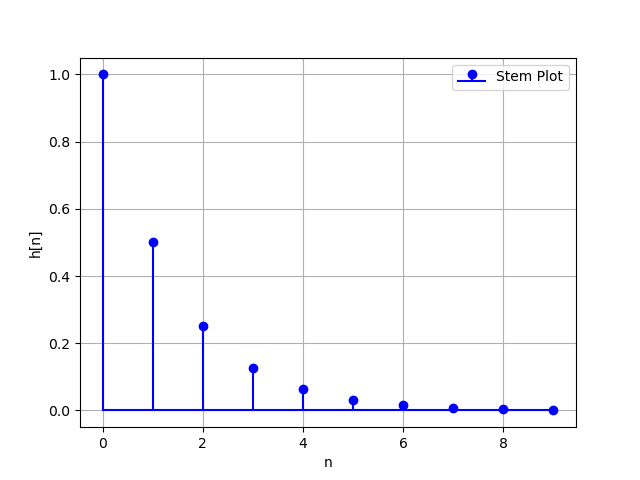
\includegraphics[width=0.5\textwidth]{2023/BM/26/figs/fig1.png}
    \caption{Plot of $h[n]$ vs $n$}
    \label{fig:GATE.2023.BM.26.1}
\end{figure}

\begin{enumerate}
\item From \eqref{eq:GATE.2023.BM.26.6} , \ref{option:GATE.2023.BM.26.1} is wrong
\item As pole lies within unit circle \ref{option:GATE.2023.BM.26.2} is true
\item From \eqref{eq:GATE.2023.BM.26.6} and \figref{fig:GATE.2023.BM.26.1} ,\ref{option:GATE.2023.BM.26.3} is true and hence
\item \ref{option:GATE.2023.BM.26.4} is false 
\end{enumerate}





%\end{document}

\newpage

\item  In the following block diagram, $R(s)$ and $D(s)$ are two inputs. The output Y(s) is expressed as $Y(s) = G_1(s)R(s) + G_2(s)D(s).$\\
$G_1(s)$ and $G_2(s)$ are given by \hfill{GATE 2023 EC Question 42}\\
\begin{figure}[htbp]
\centering
\includegraphics[width=\columnwidth]{2023/EC/42/figs/gate.png}
\end{figure}
\solution
\newpage

\item In the table shown below, match the signal type with its spectral characteristics.\hfill{GATE 2023 EC}

\vspace{2mm}

\begin{table}[ht]
    \centering
    \def\arraystretch{2.5}
    \begin{tabular}{|c|c|}
\hline
Signal Type & Spectral Characterstics \\
\hline
$\brak{i}$  Continuous, aperiodic & \brak{a} Continuous, aperiodic\\
\hline
$\brak{ii}$ Continuous, periodic & \brak{b} Continuous, periodic \\
\hline
$\brak{iii}$ Discrete, aperiodic & \brak{c} Discrete, aperiodic\\
\hline
$\brak{iii}$ Discrete, periodic & \brak{d} Discrete, periodic\\
\hline
\end{tabular}
    \caption{ }
    \label{29.2023}
\end{table}

\begin{enumerate}
\item \brak{\romannumeral 1} \textrightarrow \brak{a}  ,   \brak{\romannumeral 2} \textrightarrow \brak{b}   ,   \brak{\romannumeral 3} \textrightarrow \brak{c}   ,   \brak{\romannumeral 4} \textrightarrow \brak{d}

\item \brak{\romannumeral 1} \textrightarrow \brak{a}   ,  \brak{\romannumeral 2} \textrightarrow \brak{c}   ,   \brak{\romannumeral 3} \textrightarrow \brak{b}   ,   \brak{\romannumeral 4} \textrightarrow \brak{d}

\item  \brak{\romannumeral 1} \textrightarrow \brak{d}   ,   \brak{\romannumeral 2} \textrightarrow \brak{b}   ,   \brak{\romannumeral 3} \textrightarrow \brak{c}   ,   \brak{\romannumeral 4} \textrightarrow \brak{a}

\item \brak{\romannumeral 1} \textrightarrow \brak{a}   ,  \brak{\romannumeral 2} \textrightarrow \brak{c}    ,   \brak{\romannumeral 3} \textrightarrow \brak{d}   ,  \brak{\romannumeral 4} \textrightarrow \brak{b}

\end{enumerate}
\solution
\newpage


\item
The impulse response of an LTI system is $h\brak{t}$= $\delta\brak{t}$+0.5$ \delta\brak{t-4}$, where $\delta\brak{t}$ is continuous-time unit impulse signal.If the input signal $x(t)=\cos\brak{\frac{7\pi t}{4}}$,the output is\hfill(GATE IN 2023)\\
\solution 
\iffalse
\let\negmedspace\undefined
\let\negthickspace\undefined
\documentclass[journal,12pt,twocolumn]{IEEEtran}
\usepackage{cite}
\usepackage{amsmath,amssymb,amsfonts}
\usepackage{graphicx}
\usepackage{textcomp}
\usepackage{xcolor}
\usepackage{txfonts}
\usepackage{listings}
\usepackage{enumitem}
\usepackage{mathtools}
\usepackage{gensymb}
\usepackage{comment}
\usepackage[breaklinks=true]{hyperref}
\usepackage{tkz-euclide} 
\usepackage{listings}
\usepackage{gvv}                                        
\def\inputGnumericTable{}                                 
\usepackage[latin1]{inputenc}                                
\usepackage{color}                                            
\usepackage{array}                                            
\usepackage{longtable}                                       
\usepackage{calc}                                             
\usepackage{multirow}                                         
\usepackage{hhline}                                           
\usepackage{ifthen}                                           
\usepackage{lscape}
\usepackage[export]{adjustbox}

\newtheorem{theorem}{Theorem}[section]
\newtheorem{problem}{Problem}
\newtheorem{proposition}{Proposition}[section]
\newtheorem{lemma}{Lemma}[section]
\newtheorem{corollary}[theorem]{Corollary}
\newtheorem{example}{Example}[section]
\newtheorem{definition}[problem]{Definition}
\newcommand{\BEQA}{\begin{eqnarray}}
\newcommand{\EEQA}{\end{eqnarray}}
\newcommand{\define}{\stackrel{\triangle}{=}}
\newtheorem{rem}{Remark}

\begin{document}
\parindent 0px
\bibliographystyle{IEEEtran}

\vspace{3cm}

\title{}
\author{EE23BTECH11042 -  Khusinadha Naik$^{*}$
}
\maketitle
\newpage
\bigskip

% \renewcommand{\thefigure}{\theenumi}
% \renewcommand{\thetable}{\theenumi}


\noindent \textbf{26.} \hspace{2pt}A causal, discrete time system is described by the difference equation $y[n] = 0.5 y[n-1] + x[n]$, for all $n$, where $y[n]$ denotes the output sequence and $x[n]$ denotes the input sequence. Which of the following statements is/are TRUE?
\begin{flushright}
\hfill(GATE 2023 BM)
\end{flushright}
\begin{enumerate}[label = (\alph*)]
	\item The system has an impulse response described by $0.5^{n} u[-n]$ where $u[n]$ is the  
unit step sequence. 	\label{option:GATE.2023.BM.26.1}	
	\item The system is stable in the bounded input, bounded output sense.		\label{option:GATE.2023.BM.26.2}
	\item The system has an infinite number of non-zero samples in its impulse response	\label{option:GATE.2023.BM.26.3}
	\item The system has a finite number of non-zero samples in its impulse response.	\label{option:GATE.2023.BM.26.4}
\end{enumerate}

\noindent \textbf{Ans.}\\
\fi
\begin{table}[h]
\centering
\begin{tabular}{|c|c|c|}
        \hline
        \textbf{Parameter} & \textbf{Value} & \textbf{Description} \\
        \hline
        $x[n]$ & ? & Input Sequence \\
        \hline
        $y[n]$ & ? & Output Sequence \\
        \hline
\end{tabular}
\caption{Input parameters table}
\label{tab:GATE.2023.BM.26.1}





\end{table}
\begin{align}
y[n] = 0.5y[n-1] + x[n] 
\end{align}

Taking $Z$-Transform 
\begin{align}
Y\brak{z} &= 0.5z^{-1}Y\brak{z} + X\brak{z} \\
\implies \frac{Y\brak{z}}{X\brak{z}} &= \frac{1}{1 - 0.5z^{-1}} = H\brak{z} 
\end{align}
If $x[n]$ is impulse input 
\begin{align}
\implies &Y\brak{z} = H\brak{z} = \frac{1}{1 - 0.5z^{-1}}  \label{eq:GATE.2023.BM.26.4}
\end{align}
From \eqref{eq:GATE.2023.BM.26.4} pole lies at $z = 0.5$
\begin{align}
a^{n}u\brak{n} \xleftrightarrow{\mathcal{Z}} &\frac{1}{1 - az^{-1}} \quad , \abs{z} > a \label{eq:GATE.2023.BM.26.5}
\end{align}

From \eqref{eq:GATE.2023.BM.26.4} , \eqref{eq:GATE.2023.BM.26.5}
\begin{align}
h[n] = 0.5^{n}u[n] \quad , \abs{z} > 0.5 \label{eq:GATE.2023.BM.26.6}
\end{align}


\pagebreak
Plotting $h[n]$ vs $n$
\begin{figure}[h]
    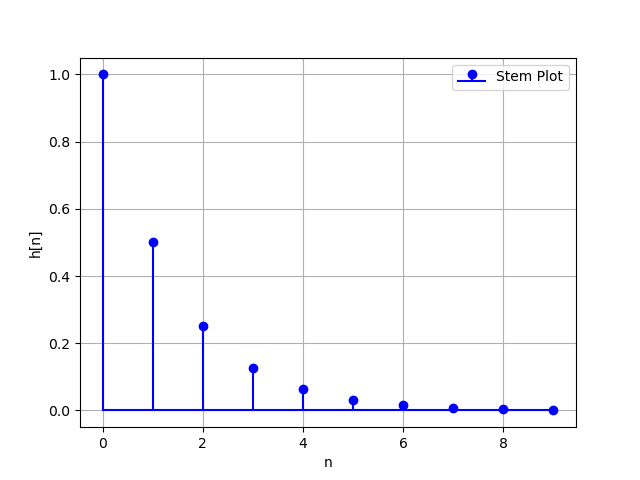
\includegraphics[width=0.5\textwidth]{2023/BM/26/figs/fig1.png}
    \caption{Plot of $h[n]$ vs $n$}
    \label{fig:GATE.2023.BM.26.1}
\end{figure}

\begin{enumerate}
\item From \eqref{eq:GATE.2023.BM.26.6} , \ref{option:GATE.2023.BM.26.1} is wrong
\item As pole lies within unit circle \ref{option:GATE.2023.BM.26.2} is true
\item From \eqref{eq:GATE.2023.BM.26.6} and \figref{fig:GATE.2023.BM.26.1} ,\ref{option:GATE.2023.BM.26.3} is true and hence
\item \ref{option:GATE.2023.BM.26.4} is false 
\end{enumerate}





%\end{document}

\newpage

\newpage

\item Consider the state-space description of an LTI system with matrices
\[ 
A = \begin{bmatrix} 0 & 1 \\ -1 & -2 \end{bmatrix}, \quad 
B = \begin{bmatrix} 0 \\ 1 \end{bmatrix}, \quad 
C = \begin{bmatrix} 3 & -2 \end{bmatrix}, \quad 
D = 1 
\]

For the input, $\sin(\omega t)$, $\omega > 0$, the value of $\omega$ for which the steady-state output of the system will be zero, is \underline{\hspace{2cm}} (Round off to the nearest integer).
\hfill(GATE 2023 EE Q46)\\
\solution
\input{2023/EE/46/gate46.tex}
\newpage

\item A causal, discrete time system is described by the difference equation $y[n] = 0.5 y[n-1] + x[n]$, for all $n$, where $y[n]$ denotes the output sequence and $x[n]$ denotes the input sequence. Which of the following statements is/are TRUE?

\begin{enumerate}[label = (\alph*)]
	\item he system has an impulse response described by $0.5^{n} u[-n]$ where $u[n]$ is the  
unit step sequence. 		
	\item The system is stable in the bounded input, bounded output sense.
	\item The system has an infinite number of non-zero samples in its impulse response
	\item The system has a finite number of non-zero samples in its impulse response.
\end{enumerate}

\hfill(GATE 2023 BM-26)\\
\solution
\newpage

\item A closed loop system is shown in the figure where $k>0$ and $\alpha>0$. The steady state
error due to a ramp input $\brak{R\brak{s} = \alpha s^{-2}}$  is given by \hfill{(GATE 2023 EC 41)}

\begin{figure}[ht]
\centering
    \includegraphics[width=1.0\linewidth]{2023/EC/41/figs/question.png}
\end{figure}
\begin{enumerate}[label = (\alph*)]
  \item $\frac{2\alpha}{k}$    
  \item $\frac{\alpha}{k}$
  \item $\frac{\alpha}{2k}$
  \item $\frac{\alpha}{4k}$
\end{enumerate}
    
\solution
\newpage

\end{enumerate}

\chapter{Sequences}
\begin{enumerate}[label=\thechapter.\arabic*,ref=\thechapter.\theenumi]

\item Consider the discrete time signal $x\sbrak{n} = u\sbrak{-n+5} - u\sbrak{n+3}$, where
\[u\sbrak{n} = 
\begin{cases}
    1;n\geq0\\
    0;n<0
\end{cases}
\]
The smallest n for which $x\sbrak{n} = 0$ is?
\hfill(GATE IN 2023)
\\ \solution
\documentclass[journal,12pt,twocolumn]{IEEEtran}

% Packages
\usepackage{cite}
\usepackage{amsmath,amssymb,amsfonts,amsthm}
\usepackage{graphicx}
\usepackage{textcomp}
\usepackage{xcolor}
\usepackage{txfonts}
\usepackage{listings}
\usepackage{enumitem}
\usepackage{mathtools}
\usepackage{float}
\usepackage{gensymb}
\usepackage{comment}
\usepackage{hyperref}
\usepackage{tkz-euclide}
\usepackage{gvv}
\usepackage[latin1]{inputenc}
\usepackage{color}
\usepackage{array}
\usepackage{longtable}
\usepackage{calc}
\usepackage{multirow}
\usepackage{hhline}
\usepackage{ifthen}
\usepackage{lscape}
\usepackage{subcaption}
\usepackage{tikz}
\usepackage{circuitikz}
\usepackage{wrapfig}
\usepackage{lipsum}
\usepackage[export]{adjustbox}
\usepackage{inputenc}

% Custom commands and macros
\newtheorem{theorem}{Theorem}[section]
\newtheorem{problem}{Problem}
\newtheorem{proposition}{Proposition}[section]
\newtheorem{lemma}{Lemma}[section]
\newtheorem{corollary}[theorem]{Corollary}
\newtheorem{example}{Example}[section]
\newtheorem{definition}[problem]{Definition}
\newtheorem{rem}{Remark}
\newcommand{\BEQA}{\begin{eqnarray}}
\newcommand{\EEQA}{\end{eqnarray}}
\newcommand{\define}{\stackrel{\triangle}{=}}
\renewcommand{\thefigure}{\theenumi}
\renewcommand{\thetable}{\theenumi}



\begin{document}

\title{GATE 2023 EC 49}
\author{EE23BTECH11045 - Palavelli Srija$^{*}$}
\maketitle

\bigskip

\textbf{Question 12.7.7:} 
Let $x(t) = 10 \cos(10.5 \omega t)$ be passed through an LTI system with impulse response $h(t) = \pi\left(\frac{\sin(\omega t)}{\pi t}\right)^2 \cos(10 \omega t)$ . The output of the system is: \\

\textbf{Solution:}
\begin{table}[h!]
    \centering
    \begin{table}[htbp]
	\centering
	\noindent
	\fontsize{10}{15}\selectfont {
		\resizebox{0.45\textwidth}{!}{%
			\begin{tabular}{|c|c|c|}
				\hline
				\textbf{Parameter} & \textbf{Value} & \textbf{Description} \\
				\hline
				$x\brak t$ & - & Input voltage \\
				\hline
				$y\brak t$ & - & Output voltage \\
				\hline
				$h\brak t$ & $\frac{y\brak t}{x\brak t}$ & Impulse response \\
				\hline
				$X\brak s$ & - & Input voltage in s-domain \\
				\hline
				$Y\brak s$ & - & Output voltage in s-domain \\
				\hline
				$H\brak s$ & $\frac{Y\brak s}{X\brak s}$ & Impulse response in s-domain \\
				\hline
			\end{tabular}
	} }
	\caption*{Input Table}
	
\end{table}
    \caption{Input Parameters}
    \label{tab:table_sr10}
\end{table}

Given \(h(t)\) is real and even. When a sinusoidal input is applied to an LTI system with an even impulse response, the output will also be sinusoidal. Hence, \(y(t) = A\cdot 10\cos(10.5 \omega t + \theta)\).

\[
x(t) \xrightarrow{\text{}} \boxed{\text{h(t)}} \xrightarrow{\text{}} y(t)
\]

\begin{align}
\text{Let } f(t) &= \pi\left(\frac{\sin(\omega t)}{\pi t}\right)^2 \\
h(t) &= f(t) \cos(10 \omega t)
\end{align}

Using 
\begin{align}
x_1(t) \cdot x_2(t) \xleftrightarrow{\mathcal{F}} X_1(\omega) * X_2(\omega)\\
\left(\frac{\sin(\omega t)}{\pi t}\right) \cdot \left(\frac{\sin(\omega t)}{\pi t}\right) \xleftrightarrow{\mathcal{F}} X_1(\omega) * X_2(\omega)
\end{align}
\begin{figure}[h!]
    \centering
    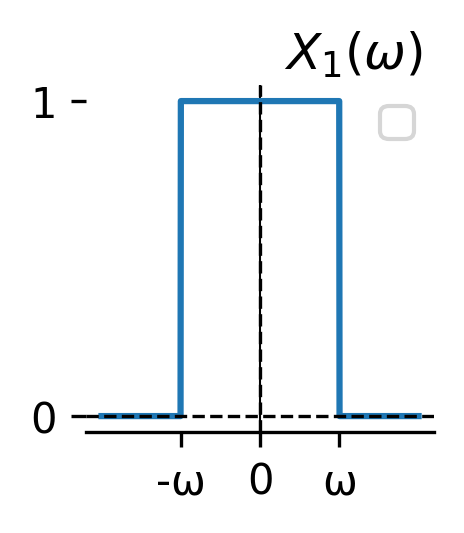
\includegraphics[width=0.4\columnwidth, height=2.5cm]{figs/plot.png}\hfill
    \begin{tabular}{c}
        {\sffamily\raisebox{1.75cm}{*}} 
    \end{tabular}\hfill
    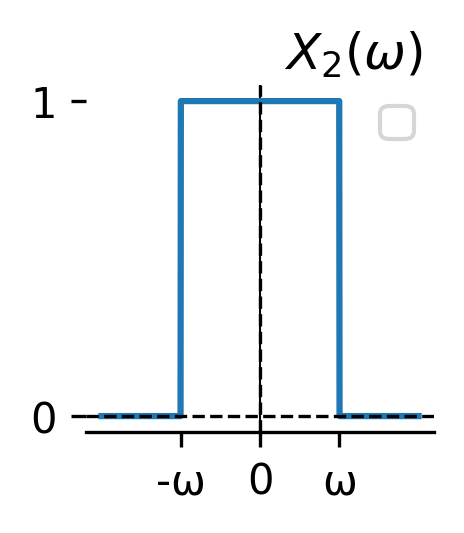
\includegraphics[width=0.4\columnwidth, height=2.5cm]{figs/plot4.png}
    
    \caption{}
    \label{fig:overall}
\end{figure}

\begin{align}
\left(\frac{\sin(\omega t)}{\pi t}\right)^2  \xleftrightarrow{\mathcal{F}} X_3(\omega) 
\end{align}
\begin{figure}[h!]
    \centering
    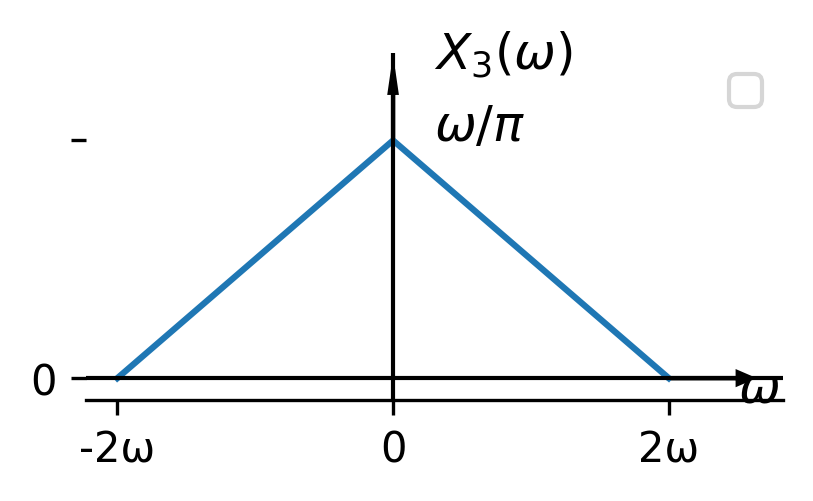
\includegraphics[width=0.5\columnwidth, height=3cm]{figs/plot1.png}
    \caption{}
    \label{fig:sr11}
\end{figure}
\begin{align}
\pi\left(\frac{\sin(\omega t)}{\pi t}\right)^2 \xleftrightarrow{\mathcal{F}} X_4(\omega)
\end{align}
\begin{figure}[h!]
    \centering
    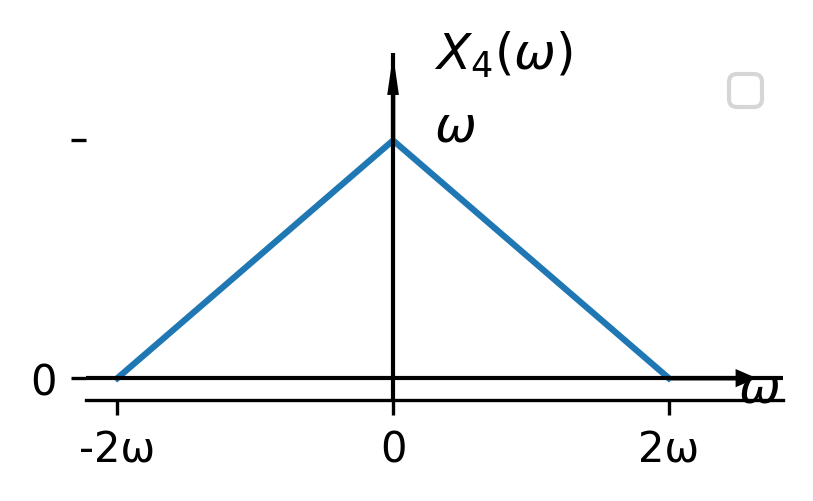
\includegraphics[width=0.5\columnwidth, height=3cm]{figs/plot2.png}
    \caption{}
    \label{fig:sr12}
\end{figure}
    \begin{align}
\text{From modulating property:} \nonumber \\
        f(t) \cos(\omega_0 t) \xleftrightarrow{\mathcal{F}} \frac{1}{2} \left[F(\omega + \omega_0) + F(\omega - \omega_0)\right]
    \end{align}

    \begin{align}
        H(\omega) &= \frac{1}{2} \left[F(\omega + 10\omega) + F(\omega - 10\omega)\right]
    \end{align}

\begin{figure}[h!]
    \centering
    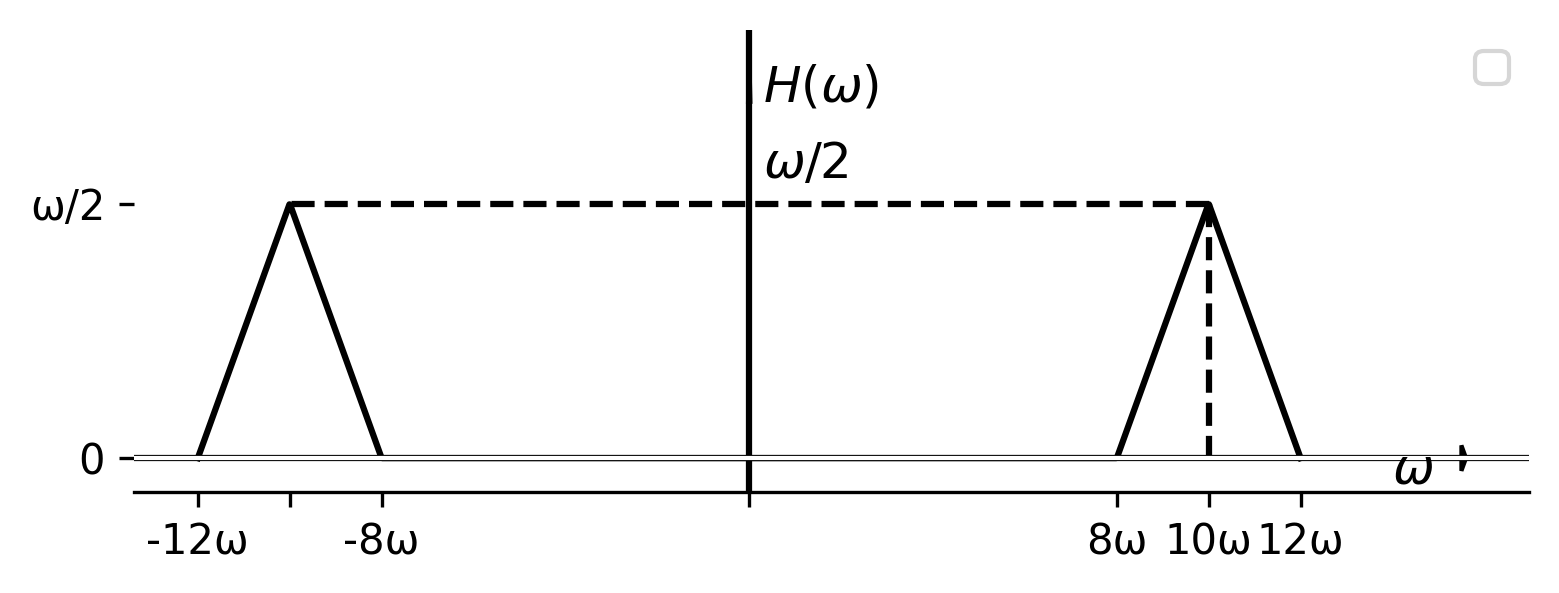
\includegraphics[width=0.7\columnwidth,height=2.5cm]{figs/plot3.png}
    \caption{}
    \label{fig:sr13}
\end{figure}
\begin{equation}
    \frac{\frac{\omega}{2} - 0}{10\omega - 12\omega} = \frac{|H(10.5\omega)| - 0}{10.5\omega - 12\omega}
\end{equation}

\begin{align}
A = |H(10.5\omega)| &= \frac{3}{8}\omega \quad \text{and} \quad  \theta= \angle H(10.5\omega) = 0^\circ
\end{align}

The output \(y(t)\):
\begin{align}
y(t) &= \frac{3}{8}\omega \cdot 10 \cos(10.5 \omega t) \\
&= \frac{15}{4}\omega \cos(10.5 \omega t)
\end{align}
\begin{figure}[h!]
    \centering
    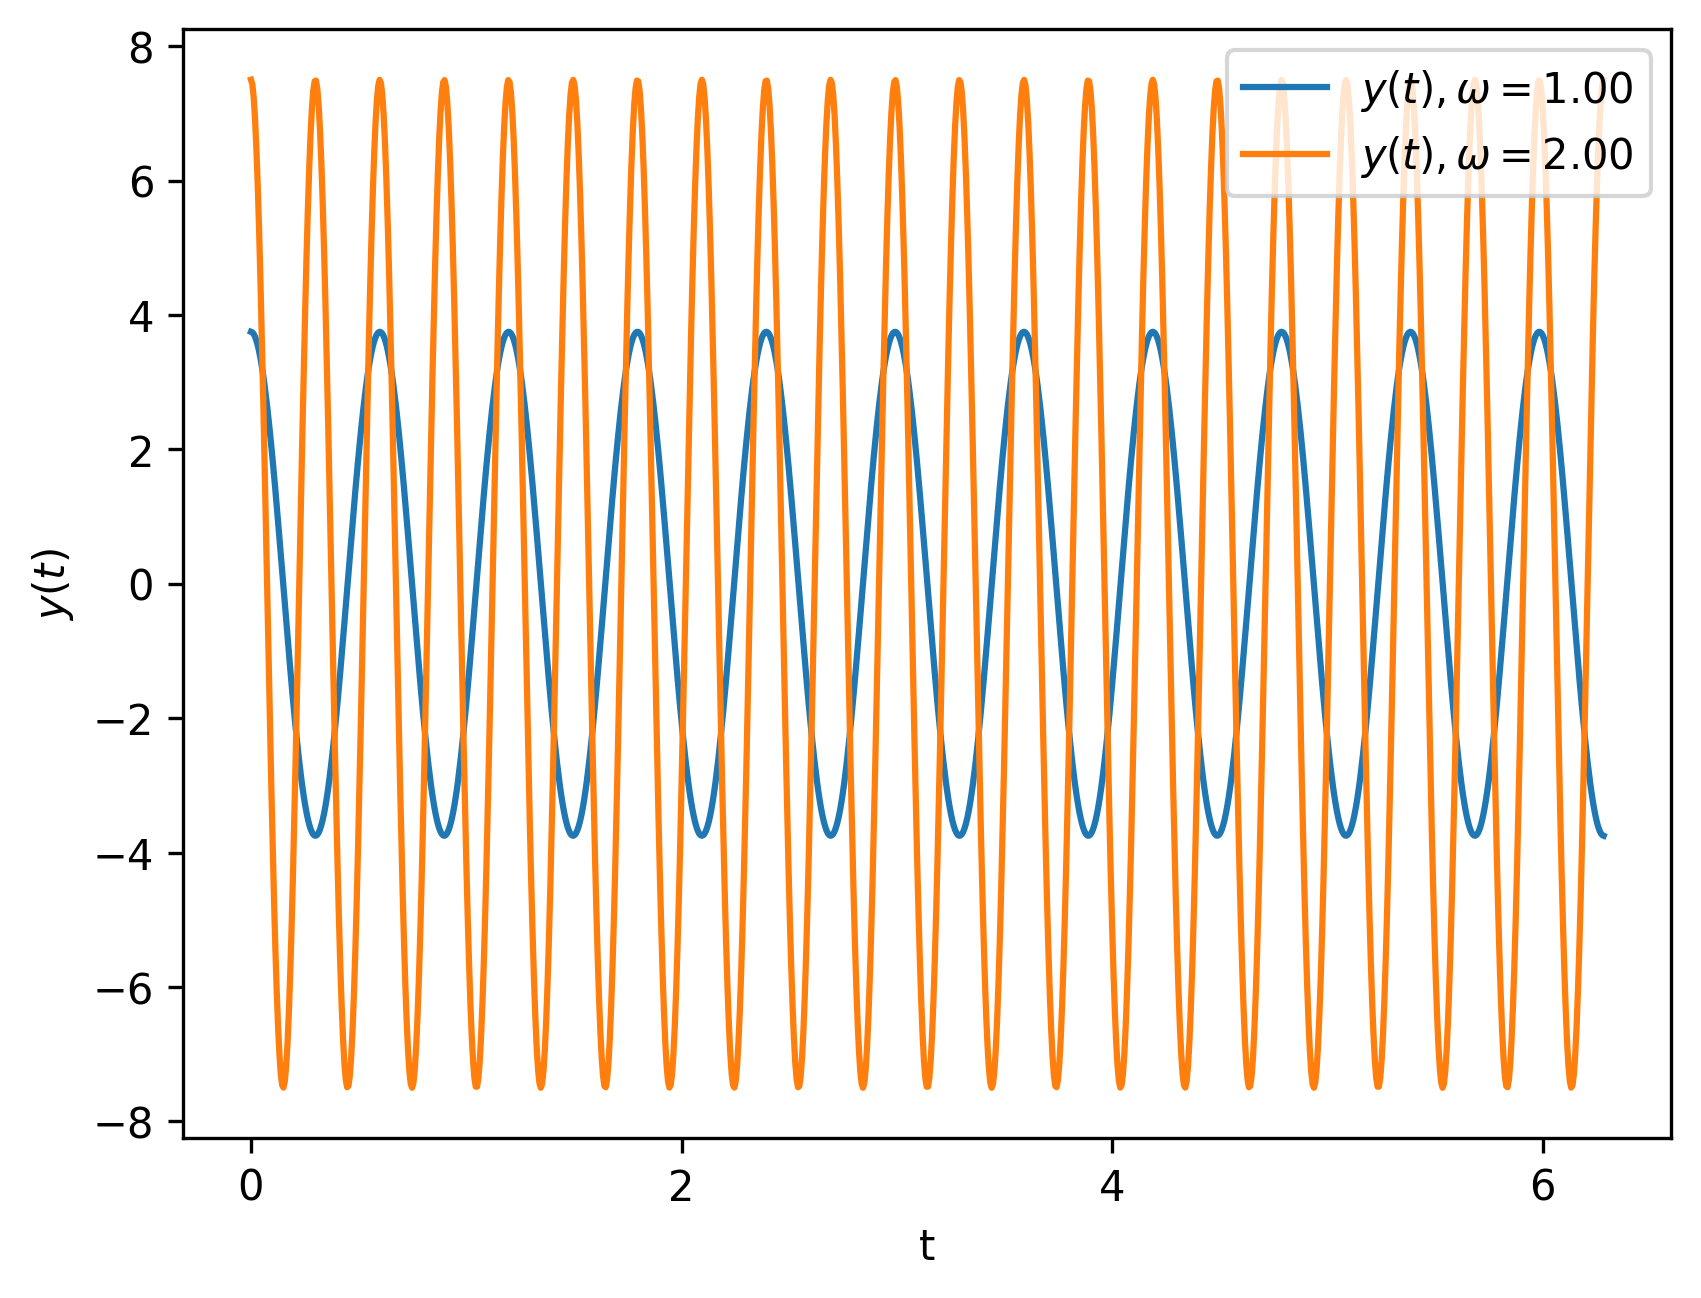
\includegraphics[width=\columnwidth]{figs/plot5.png}
    \caption{}
    \label{fig:sr14}
\end{figure}
\end{document}


\newpage
\item Two sequences $x_1\sbrak{n} $ and $ x_2 \sbrak{n}$ are described as follows:
\begin{align}
x_1\sbrak{0} = x_2\sbrak{0} = 1\\
x_1\sbrak{1} = x_2\sbrak{2} = 2\\
x_1\sbrak{2} = x_2\sbrak{1} = 1
\end{align}
$x_1\sbrak{n} = x_2\sbrak{n} = 0$ for all $n<0$ and $n>2$\\
\\
If $x\sbrak{n}$ is obtained by convoluting $x_1\sbrak{n}$ with $x_2\sbrak{n}$, which of the following equations is/are TRUE?\\
\\
(A) $x\sbrak{2} = x\sbrak{3}$\\
\\
(B) $x\sbrak{1} = 2$\\
\\
(C) $x\sbrak{4} = 3$\\
\\
(D) $x\sbrak{2} = 5$\\
\hfill(GATE 2023 BM 47)
\solution
\input {2023/BM/47/Gate2023_Bm_47.tex}
\pagebreak
\item A series \brak{S} is given as S=1+3+5+7+9+..... The sum of the first 50 terms of S is \underline{\hspace{1in}}
\hfill(GATE 2023 BT 32)
\\ \solution
\iffalse
\let\negmedspace\undefined
\let\negthickspace\undefined
\documentclass[journal,12pt,twocolumn]{IEEEtran}
\usepackage{cite}
\usepackage{amsmath,amssymb,amsfonts}
\usepackage{graphicx}
\usepackage{textcomp}
\usepackage{xcolor}
\usepackage{txfonts}
\usepackage{listings}
\usepackage{enumitem}
\usepackage{mathtools}
\usepackage{gensymb}
\usepackage{comment}
\usepackage[breaklinks=true]{hyperref}
\usepackage{tkz-euclide} 
\usepackage{listings}
\usepackage{gvv}                                        
\def\inputGnumericTable{}                                 
\usepackage[latin1]{inputenc}                                
\usepackage{color}                                            
\usepackage{array}                                            
\usepackage{longtable}                                       
\usepackage{calc}                                             
\usepackage{multirow}                                         
\usepackage{hhline}                                           
\usepackage{ifthen}                                           
\usepackage{lscape}
\usepackage[export]{adjustbox}

\newtheorem{theorem}{Theorem}[section]
\newtheorem{problem}{Problem}
\newtheorem{proposition}{Proposition}[section]
\newtheorem{lemma}{Lemma}[section]
\newtheorem{corollary}[theorem]{Corollary}
\newtheorem{example}{Example}[section]
\newtheorem{definition}[problem]{Definition}
\newcommand{\BEQA}{\begin{eqnarray}}
\newcommand{\EEQA}{\end{eqnarray}}
\newcommand{\define}{\stackrel{\triangle}{=}}
\newtheorem{rem}{Remark}

\begin{document}
\parindent 0px
\bibliographystyle{IEEEtran}

\vspace{3cm}

\title{}
\author{EE23BTECH11042 -  Khusinadha Naik$^{*}$
}
\maketitle
\newpage
\bigskip

% \renewcommand{\thefigure}{\theenumi}
% \renewcommand{\thetable}{\theenumi}


\noindent \textbf{26.} \hspace{2pt}A causal, discrete time system is described by the difference equation $y[n] = 0.5 y[n-1] + x[n]$, for all $n$, where $y[n]$ denotes the output sequence and $x[n]$ denotes the input sequence. Which of the following statements is/are TRUE?
\begin{flushright}
\hfill(GATE 2023 BM)
\end{flushright}
\begin{enumerate}[label = (\alph*)]
	\item The system has an impulse response described by $0.5^{n} u[-n]$ where $u[n]$ is the  
unit step sequence. 	\label{option:GATE.2023.BM.26.1}	
	\item The system is stable in the bounded input, bounded output sense.		\label{option:GATE.2023.BM.26.2}
	\item The system has an infinite number of non-zero samples in its impulse response	\label{option:GATE.2023.BM.26.3}
	\item The system has a finite number of non-zero samples in its impulse response.	\label{option:GATE.2023.BM.26.4}
\end{enumerate}

\noindent \textbf{Ans.}\\
\fi
\begin{table}[h]
\centering
\begin{tabular}{|c|c|c|}
        \hline
        \textbf{Parameter} & \textbf{Value} & \textbf{Description} \\
        \hline
        $x[n]$ & ? & Input Sequence \\
        \hline
        $y[n]$ & ? & Output Sequence \\
        \hline
\end{tabular}
\caption{Input parameters table}
\label{tab:GATE.2023.BM.26.1}





\end{table}
\begin{align}
y[n] = 0.5y[n-1] + x[n] 
\end{align}

Taking $Z$-Transform 
\begin{align}
Y\brak{z} &= 0.5z^{-1}Y\brak{z} + X\brak{z} \\
\implies \frac{Y\brak{z}}{X\brak{z}} &= \frac{1}{1 - 0.5z^{-1}} = H\brak{z} 
\end{align}
If $x[n]$ is impulse input 
\begin{align}
\implies &Y\brak{z} = H\brak{z} = \frac{1}{1 - 0.5z^{-1}}  \label{eq:GATE.2023.BM.26.4}
\end{align}
From \eqref{eq:GATE.2023.BM.26.4} pole lies at $z = 0.5$
\begin{align}
a^{n}u\brak{n} \xleftrightarrow{\mathcal{Z}} &\frac{1}{1 - az^{-1}} \quad , \abs{z} > a \label{eq:GATE.2023.BM.26.5}
\end{align}

From \eqref{eq:GATE.2023.BM.26.4} , \eqref{eq:GATE.2023.BM.26.5}
\begin{align}
h[n] = 0.5^{n}u[n] \quad , \abs{z} > 0.5 \label{eq:GATE.2023.BM.26.6}
\end{align}


\pagebreak
Plotting $h[n]$ vs $n$
\begin{figure}[h]
    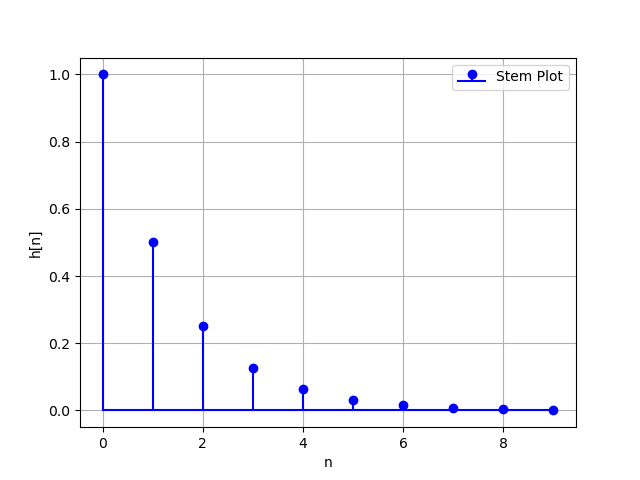
\includegraphics[width=0.5\textwidth]{2023/BM/26/figs/fig1.png}
    \caption{Plot of $h[n]$ vs $n$}
    \label{fig:GATE.2023.BM.26.1}
\end{figure}

\begin{enumerate}
\item From \eqref{eq:GATE.2023.BM.26.6} , \ref{option:GATE.2023.BM.26.1} is wrong
\item As pole lies within unit circle \ref{option:GATE.2023.BM.26.2} is true
\item From \eqref{eq:GATE.2023.BM.26.6} and \figref{fig:GATE.2023.BM.26.1} ,\ref{option:GATE.2023.BM.26.3} is true and hence
\item \ref{option:GATE.2023.BM.26.4} is false 
\end{enumerate}





%\end{document}

\pagebreak

\item For the signals x\brak{t} and y\brak{t} shown in the figure, $z\brak{t}=x\brak{t}*y\brak{t}$ is maximum at $t=T_1$. Then $T_1$ in seconds is .......... \brak{\text{Round off to the nearest integer}}
\solution
\pagebreak

\item A series of natural numbers F$_1$, F$_2$, F$_3$, F$_4$, F$_5$, F$_6$, F$_7$,....obeys F$_{n+1}$ = F$_n$ + F$_{n-1}$ for all integers n $\geq$ 2. If F$_6$ = 37, and F$_7$ = 60, then what is F$_1$?\\  
 \hfill[GATE CS 2023] \\
 \solution 
 iffalse
\let\negmedspace\undefined
\let\negthickspace\undefined
\documentclass[journal,12pt,onecolumn]{IEEEtran}
\usepackage{cite}
\usepackage{amsmath,amssymb,amsfonts}
\usepackage{graphicx}
\usepackage{textcomp}
\usepackage{xcolor}
\usepackage{txfonts}
\usepackage{listings}
\usepackage{enumitem}
\usepackage{mathtools}
\usepackage{gensymb}
\usepackage{comment}
\usepackage[breaklinks=true]{hyperref}
\usepackage{tkz-euclide} 
\usepackage{listings}
\usepackage{gvv}                                        
\def\inputGnumericTable{}                                 
\usepackage[latin1]{inputenc}                                
\usepackage{color}                                            
\usepackage{array}                                            
\usepackage{longtable}                                       
\usepackage{calc}                                             
\usepackage{multirow}                                         
\usepackage{hhline}                                           
\usepackage{ifthen}                                           
\usepackage{lscape}
\usepackage[export]{adjustbox}
\newtheorem{theorem}{Theorem}[section]
\newtheorem{problem}{Problem}
\newtheorem{proposition}{Proposition}[section]
\newtheorem{lemma}{Lemma}[section]
\newtheorem{corollary}[theorem]{Corollary}
\newtheorem{example}{Example}[section]
\newtheorem{definition}[problem]{Definition}
\newcommand{\BEQA}{\begin{eqnarray}}
	\newcommand{\EEQA}{\end{eqnarray}}
\newcommand{\define}{\stackrel{\triangle}{=}}
\newtheorem{rem}{Remark}

\begin{document}
	\parindent 0px
	\bibliographystyle{IEEEtran}
	

	
	\title{}
	\author{EE23BTECH11209 - K S Ballvardhan$^{*}$
	}
	\maketitle
	\bigskip
	
	% \renewcommand{\thefigure}{\theenumi}
	% \renewcommand{\thetable}{\theenumi}
	
	
	
	
	\textbf{Question:} A series of natural numbers F$_1$, F$_2$, F$_3$, F$_4$, F$_5$, F$_6$, F$_7$,....obeys F$_{n+1}$ = F$_n$ + F$_{n-1}$ for all integers n $\geq$ 2.
	If F$_6$ = 37, and F$_7$ = 60, then what is F$_1$? \hfill[GATE CS 2023]
	
	\textbf{Solution: }
	
	\begin{table}[ht] 
		\centering
		\begin{tabular}{|c|c|c|}
    \hline
    \textbf{Parameter} & \textbf{Description} & \textbf{Value} \\
    \hline
    $ x\brak 6$ & Seventh term of the sequence & 60 \\
    \hline
    $ x\brak 5$ & Sixth term of the sequence & 37 \\
    \hline
    $ x\brak 1$ & Second term of the sequence & ? \\
    \hline
    $ x\brak 0$ & First term of the sequence & ? \\
    \hline
    \end{tabular}


		\caption{input values}
		\label{tab: Table2023cs3}
	\end{table}
	
    Taking z-transform of $X\brak z$:
	\begin{align}
		X\brak{z} &= x\brak 0 + z^{-1} x\brak 1 + \sum_{n=2}^{\infty} x\brak n z^{-n}\\
	    &= x\brak 0 + z^{-1} x\brak 1 + z^{-1} \sum_{n=1}^{\infty} x\brak {n+1} z^{-n}\\
	    &= x\brak 0 + z^{-1} x\brak 1 + z^{-1} \sum_{n=1}^{\infty} \brak{x\brak n + x\brak {n-1}}z^{-n} \\
	    &= x\brak 0 + z^{-1} x\brak 1 + z^{-1}\brak{X\brak{z}-x\brak 1 + z^{-1}X\brak{z}} \\
		\implies X\brak{z}&= \frac{x\brak 0 + \brak{x\brak 1-x\brak 0}z^{-1}}{1-z^{-1}-z^{-2}}
	\end{align}
	Using Contour Integration to find the inverse $Z$-transform,
	\begin{align}
		x\brak n &=\frac{1}{2\pi j}\oint_{C} X\brak{z} \;z^{n-1} \;dz  \\
		&=\frac{1}{2\pi j}\oint_{C}\frac{z^{n}\brak{x\brak 1-x\brak 0+x\brak 0 z}}{z^2-z-1} \;dz 
	\end{align}
	
	By residue theorem:
	
	\begin{align}
		x\brak n &=\frac{1}{\brak {0}!}\lim\limits_{z\to {\frac{1+\sqrt{5}}{2}}}\frac{d}{dz}\brak {{(z+\frac{1+\sqrt{5}}{2})}X\brak{z}} + \frac{1}{\brak {0}!}\lim\limits_{z\to \frac{1-\sqrt{5}}{2}}\frac{d}{dz}\brak {{\brak{z+\frac{1-\sqrt{5}}{2}}}X\brak{z}}
	\end{align}
	On simplifying we get,
	\begin{align}
		x\brak n &= \brak{x\brak1-x\brak0}\brak{\brak{\frac{1+\sqrt{5}}{2}}^n-\brak{\frac{1-\sqrt{5}}{2}}^n} + \brak{x\brak 0}\brak{\brak{\frac{1+\sqrt{5}}{2}}^{n+1}-\brak{\frac{1-\sqrt{5}}{2}}^{n+1}}
	\end{align}
	From the values in \tabref{tab: Table2023cs3}:
	\begin{align}
		5 \brak{x\brak 1-x\brak 0} + 8 x\brak 0 &=37\\
		8 \brak{x\brak 1-x\brak 0} + 13 x\brak 0 &=60\\
		\implies x\brak 1 =5, x\brak 0 &=4
	\end{align}
	\begin{align}
		\therefore {x\brak 0=4}
	\end{align}
	\begin{figure}[ht]
		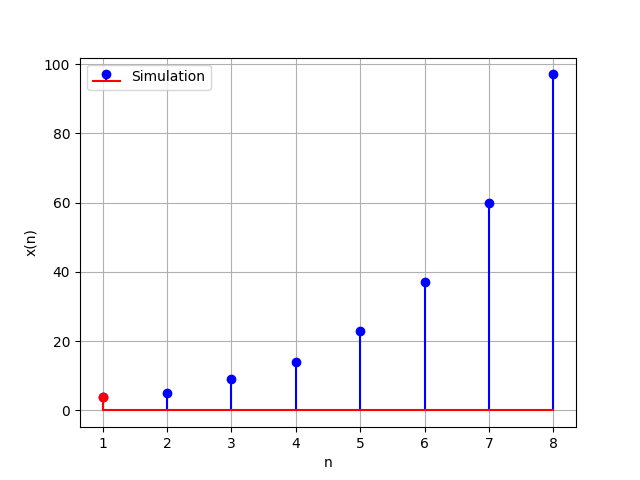
\includegraphics[width = \columnwidth]{2023/CS/3/figs/fig4.png}
		\caption{Terms of the given sequence}
		\centering
		\label{fig: fig4}
	\end{figure}
%\end{document}

 \pagebreak

 \item The Lucas sequence $L_{n}$is defined by the recurrence relation:\\
\begin{align*}
    L_{n}=L_{n-1}+L_{n-2}, for n\geq3
\end{align*}
with $L_{1}$=1 and $L_{2}$=3\\
Which one of the option given is TRUE?\\
\begin{enumerate}
    \item $L_{n}=\brak{\frac{1+\sqrt{5}}{2}}^n+\brak{\frac{1-\sqrt{5}}{2}}^n$
    \item $L_{n}=\brak{\frac{1+\sqrt{5}}{2}}^n-\brak{\frac{1-\sqrt{5}}{3}}^n$
    \item $L_{n}=\brak{\frac{1+\sqrt{5}}{2}}^n+\brak{\frac{1-\sqrt{5}}{3}}^n$
    \item $L_{n}=\brak{\frac{1+\sqrt{5}}{2}}^n-\brak{\frac{1-\sqrt{5}}{2}}^n$
\end{enumerate}
\hfill{(GATE 2023 CS 15)}\\
\solution
\iffalse
\let\negmedspace\undefined
\let\negthickspace\undefined
\documentclass[journal,12pt,twocolumn]{IEEEtran}
\usepackage{cite}
\usepackage{amsmath,amssymb,amsfonts,amsthm}
\usepackage{algorithmic}
\usepackage{graphicx}
\usepackage{textcomp}
\usepackage{xcolor}
\usepackage{txfonts}
\usepackage{listings}
\usepackage{enumitem}
\usepackage{mathtools}
\usepackage{gensymb}
\usepackage{comment}
\usepackage[breaklinks=true]{hyperref}
\usepackage{tkz-euclide} 
\usepackage{listings}
\usepackage{gvv}                                        
\def\inputGnumericTable{}                                 
\usepackage[latin1]{inputenc}                                
\usepackage{color}                                            
\usepackage{array}                                            
\usepackage{longtable}                                       
\usepackage{calc}                                             
\usepackage{multirow}                                         
\usepackage{hhline}                                           
\usepackage{ifthen}                                           
\usepackage{lscape}
\newtheorem{theorem}{Theorem}[section]
\newtheorem{problem}{Problem}
\newtheorem{proposition}{Proposition}[section]
\newtheorem{lemma}{Lemma}[section]
\newtheorem{corollary}[theorem]{Corollary}
\newtheorem{example}{Example}[section]
\newtheorem{definition}[problem]{Definition}
\newcommand{\BEQA}{\begin{eqnarray}}
\newcommand{\EEQA}{\end{eqnarray}}
\newcommand{\define}{\stackrel{\triangle}{=}}
\theoremstyle{remark}
\newtheorem{rem}{Remark}
\begin{document}
\parindent 0px
\bibliographystyle{IEEEtran}
\title{Assignment CS\_15Q}
\author{EE23BTECH11028 - Kamale Goutham$^{}$% <-this % stops a space
}
\maketitle
\newpage
\bigskip
\section*{Question}
The Lucas sequence $L_{n}$is defined by the recurrence relation:\\
\begin{align*}
    L_{n}=L_{n-1}+L_{n-2}, for n\geq3
\end{align*}
with $L_{1}$=1 and $L_{2}$=3\\
Which one of the option given is TRUE?\\
\begin{enumerate}
    \item $L_{n}=\brak{\frac{1+\sqrt{5}}{2}}^n+\brak{\frac{1-\sqrt{5}}{2}}^n$
    \item $L_{n}=\brak{\frac{1+\sqrt{5}}{2}}^n-\brak{\frac{1-\sqrt{5}}{3}}^n$
    \item $L_{n}=\brak{\frac{1+\sqrt{5}}{2}}^n+\brak{\frac{1-\sqrt{5}}{3}}^n$
    \item $L_{n}=\brak{\frac{1+\sqrt{5}}{2}}^n-\brak{\frac{1-\sqrt{5}}{2}}^n$
\end{enumerate}
\hfill{(GATE 2023 CS 15)}\\
\solution\\
\fi
Initial condition $L_{1}$=1 and $L_{2}$=3
\begin{align}
 L_{n}=L_{n-1}+L_{n-2}
\end{align}
Assume $L_{n+1}=x(n)$\\
\begin{align}
 x(n)=&[x(n-1)+x(n-2)-3]u(n-2)+u(n)+2u(n-1)\\
 X(z)=&z^{-1}(X(z)-1)+z^{-2}X(z)-3\frac{z^{-2}}{1-z^{-1}}+\frac{1}{1-z^{-1}}+2\frac{z^{-1}}{1-z^{-1}}\\
 X(z)&(1-z^{-1}-z^{-2})(1-z^{-1})=1+z^{-1}-2z^{-2}\\
 X(z)&=\frac{1+z^{-1}-2z^{-2}}{(1-z^{-1}-z^{-2})(1-z^{-1})}\\
 X(z)&=\frac{A}{1-z^{-1}}+\frac{B}{1-\alpha z^{-1}}+\frac{C}{1-\beta z^{-1}}
 \end{align}
 Where, $\alpha$ = $\dfrac{1 +\sqrt{5}}{2}$ and $\beta$ = $\dfrac{1 -\sqrt{5}}{2}$ \\
 
	\vspace{0.4cm}
 using partial fractions,
 \begin{align}
     X(z)=\frac{\alpha+2}{(\alpha-\beta)(1-\alpha z^{-1})}+\frac{\beta+2}{(\beta-\alpha)(1-\beta z^{-1})}
 \end{align}
 
	$a^n u(n)$
	$\xleftarrow[]{\hspace{0.4cm}{\mathcal{Z}}\hspace{0.1cm}}\xrightarrow[]{}$
	$\dfrac{1}{1 - a z^{-1}}$ \hspace{0.2cm} $\lvert \hspace{0.1cm} z \hspace{0.1cm}\rvert \hspace{0.1cm} \textgreater \hspace{0.1cm} \lvert \hspace{0.1cm} a \hspace{0.1cm} \rvert$
	
	\vspace{0.4cm}
	
	Substituting this result,
	
	\vspace{-0.5cm}
	
	\begin{align}
		x(n) &= \dfrac{\alpha+2}{(\alpha - \beta)} (\alpha^n u(n)) - \dfrac{\beta+2}{(\alpha - \beta)} (\beta^n u(n))\\
	    x(n) &= \dfrac{(5+\sqrt{5})(1 + \sqrt{5})^{n} - (5-\sqrt{5})(1 - \sqrt{5})^{n} }{2^{n+1} \sqrt{5}} u(n)\\
    	x(n) &= \dfrac{(1 + \sqrt{5})^{n+1} +(1 - \sqrt{5})^{n+1} }{2^{n+1}} u(n)
    \end{align}
$\therefore$ $L_{n} =\brak{\frac{1+\sqrt{5}}{2}}^n+\brak{\frac{1-\sqrt{5}}{2}}^n$
option 1 is correct.
\newpage
\begin{figure}[h]
  \centering
  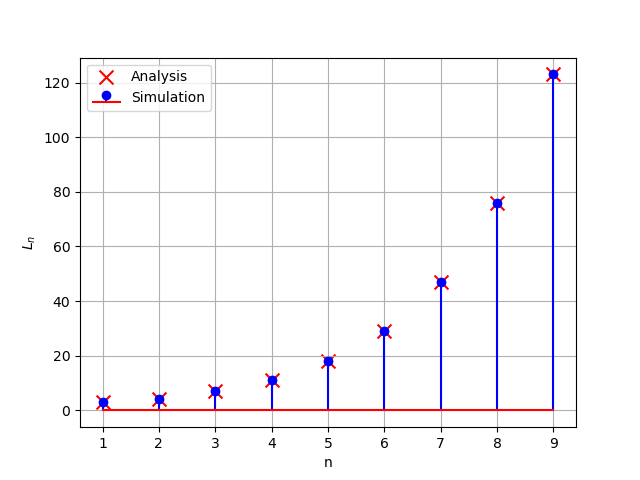
\includegraphics[width=\columnwidth]{2023/CS/15/figs/fig1.png}
  \caption{$L_{n}=\brak{\frac{1+\sqrt{5}}{2}}^n+\brak{\frac{1-\sqrt{5}}{2}}^n$}
  \label{fig:graph}
\end{figure}

\pagebreak
\end{enumerate}

\chapter{Sampling}
\begin{enumerate}[label=\thechapter.\arabic*,ref=\thechapter.\theenumi]

\item An $8$ bit ADC converts analog voltage in the range of $0$ to $+5\, V$ to the corresponding digital code as per the conversion characteristics shown in figure. For $V_{in} = 1.9922\, V$, which of the following digital output, given in hex, is true?

\begin{figure}[!h]
    \centering
    \includegraphics[width=\columnwidth]{2023/EE/40/figs/fig1.jpeg}
    \caption{}
    \label{fig:ADC_gate.ee.23.40}
\end{figure}
\begin{enumerate}[label=(\alph*)]
    \item $64H$
    \item $65H$
    \item $66H$
    \item $67H$
\end{enumerate} \hfill(GATE EE 40)

\solution
\input{2023/EE/40/GATE_EE_23_40.tex}
\newpage
\item Let x1\brak{t} and x2\brak{t} be two band-limited signals having bandwidth B = $4\pi\times10^3$
rad/s each. In the figure below, the Nyquist sampling frequency, in
rad/s, required to sample y\brak{t}, is
 \begin{circuitikz}
     \draw (0,0) node[left] {$x_1(t)$} to (0.8,0);
     \draw (0,-1) node[left] {$x_2(t)$} to (0.8,-1);
     \draw (1,0) circle(0.2);
     \draw (1,0) node {$\times$};
     \draw (1,-1) circle(0.2);
     \draw (1,-1) node {$\times$};
    \draw (1.2,0) to (1.8,0);
    \draw (1.2,-1) to (1.8,-1);
    \draw (1.8,0) to (1.8,-0.3);
    \draw (1.8,-1) to (1.8,-0.7);
    \draw (1.8,-0.5) circle(0.2);
    \draw (1.8,-0.5) node {$+$};
    \draw[->] (1,0.5) to (1,0.2) ;
    \node at (1,0.6) {cos$(4\pi\times10^3t)$};
    \draw[->] (1,-1.5) to (1,-1.2);
    \node at (1,-1.6) {cos$(12\pi\times10^3t)$};
    \draw (2,-0.5) to (2.3,-0.5);
    \node at (2.6,-0.5) {y(t)};
     
     
\end{circuitikz}
 \\
\begin{enumerate}[label=(\alph*)]
    \item $20\pi\times10^3$
    \item $40\pi\times10^3$
    \item $8\pi\times10^3$
    \item $32\pi\times10^3$
\end{enumerate} \hfill(GATE EC 50)


\solution
\iffalse
\let\negmedspace\undefined
\let\negthickspace\undefined
\documentclass[journal,12pt,twocolumn]{IEEEtran}
\usepackage{cite}
\usepackage{amsmath,amssymb,amsfonts,amsthm}
\usepackage{algorithmic}
\usepackage{graphicx}
\usepackage{textcomp}
\usepackage{xcolor}
\usepackage{txfonts}
\usepackage{listings}
\usepackage{enumitem}
\usepackage{mathtools}
\usepackage{gensymb}
\usepackage{comment}
\usepackage[breaklinks=true]{hyperref}
\usepackage{tkz-euclide} 
\usepackage{listings}
\usepackage{gvv}                                        
\def\inputGnumericTable{}                                 
\usepackage[latin1]{inputenc}                         
\usepackage{circuitikz}
\usepackage{color}                                            
\usepackage{array}                                            
\usepackage{longtable}                                       
\usepackage{calc}                                             
\usepackage{multirow} 

\usepackage{hhline}                                           
\usepackage{ifthen}                                           
\usepackage{lscape}


\newtheorem{theorem}{Theorem}[section]
\newtheorem{problem}{Problem}
\newtheorem{proposition}{Proposition}[section]
\newtheorem{lemma}{Lemma}[section]
\newtheorem{corollary}[theorem]{Corollary}
\newtheorem{example}{Example}[section]
\newtheorem{definition}[problem]{Definition}
\newcommand{\BEQA}{\begin{eqnarray}}
\newcommand{\EEQA}{\end{eqnarray}}
\newcommand{\define}{\stackrel{\triangle}{=}}
\theoremstyle{remark}
\newtheorem{rem}{Remark}


\begin{document}
\parindent 0px
\bibliographystyle{IEEEtran}

\title{GATE 2023 - EC 50}
\author{EE23BTECH11220 - R.V.S.S Varun$^{}$% <-this % stops a space
}
\maketitle
\newpage
\bigskip

\renewcommand{\thefigure}{\theenumi}
\renewcommand{\thetable}{\theenumi}
\section*{Question}

Let $x_1\brak{t}$ and $x_2\brak{t}$ be two band-limited signals having bandwidth B = $4\pi\times10^3$
rad/s each. In the figure below, the Nyquist sampling frequency, in
rad/s, required to sample y\brak{t}, is
  \\
  \vspace{25pt}
\begin{figure}[ht]
    \centering
	\begin{circuitikz}
    \begin{circuitikz}
     \draw (0,0) node[left] {$x_1(t)$} to (0.8,0);
     \draw (0,-1) node[left] {$x_2(t)$} to (0.8,-1);
     \draw (1,0) circle(0.2);
     \draw (1,0) node {$\times$};
     \draw (1,-1) circle(0.2);
     \draw (1,-1) node {$\times$};
    \draw (1.2,0) to (1.8,0);
    \draw (1.2,-1) to (1.8,-1);
    \draw (1.8,0) to (1.8,-0.3);
    \draw (1.8,-1) to (1.8,-0.7);
    \draw (1.8,-0.5) circle(0.2);
    \draw (1.8,-0.5) node {$+$};
    \draw[->] (1,0.5) to (1,0.2) ;
    \node at (1,0.6) {cos$(4\pi\times10^3t)$};
    \draw[->] (1,-1.5) to (1,-1.2);
    \node at (1,-1.6) {cos$(12\pi\times10^3t)$};
    \draw (2,-0.5) to (2.3,-0.5);
    \node at (2.6,-0.5) {y(t)};
     
     
\end{circuitikz}

	\end{circuitikz}
    \label{fig:EC50.1}
\end{figure} 

    \brak{a} $20\pi\times10^3$\\
    \brak{b} $40\pi\times10^3$\\
    \brak{c} $8\pi\times10^3$\\
    \brak{d} $32\pi\times10^3$   \hfill(GATE EC 50)\\




\fi

\begin{table}[ht]
    \centering
    \begin{tabular}{|c|c|c|}
    \hline
	Symbol &Description&Value \\
        \hline
	$f_1$&Frequency of cos$\brak{4\pi\times10^3}$&$2\times10^3$ \\
        \hline
	$f_2$&Frequency of cos$\brak{12\pi\times10^3}$&$6\times10^3$ \\
	\hline
	$f_m$&Maximum frequency of the output signal&- \\
	\hline
	 $\omega_{m}$&-&$2\pi f_m$ \\
         \hline
	 $\omega_{s}$&Nyquist sampling rate&$2\omega_m$ \\
         \hline
    \end{tabular}
 
    \caption{Table of parameters}
    \label{tab:EC50.1}
\end{table}


\begin{figure}[ht]
    \centering
	
    \begin{circuitikz}
    \draw[->] (-5,0) to (5,0);
    \draw[->] (0,-1) to (0,5);
    \draw (-3,0) to (0,3);
    \draw (0,3) to (3,0);
    \draw (-3,-0.5) node {$-2\times10^3$};
    \draw (3,-0.5) node {$2\times10^3$};
    \draw (0,5.5) node {$X_{1}\brak{f}$};

\end{circuitikz}

	
    \label{fig:EC50.2}
\end{figure} 


\begin{figure}[ht]
    \centering
	
    \begin{circuitikz}
    \draw[->] (-5,0) to (5,0);
    \draw[->] (0,-1) to (0,5);
    \draw (-3,0) to (0,3);
    \draw (0,3) to (3,0);
    \draw (-3,-0.5) node {$-2\times10^3$};
    \draw (3,-0.5) node {$2\times10^3$};
    \draw (0,5.5) node {$X_{2}\brak{f}$};
\end{circuitikz}

	
    \label{fig:EC50.3}
\end{figure} 

 From question figure ,
\begin{align}
y\brak{t}=x_1\brak{t}\times cos\brak{4\pi\times10^3t}+x_2\brak{t}\times cos\brak{12\pi\times10^3t}
\end{align}
\begin{align}
	y\brak{t}=y_1\brak{t}+y_2\brak{t}\\
	Y\brak{f}=Y_1\brak{f}+Y_2\brak{f}\label{EC50.1}
\end{align}
\begin{align}
	Y_1\brak{f}&=X_1\brak{f}*\frac{1}{2}[\delta\brak{f-f_1}+\delta\brak{f+f_1}]\\
	      &=\frac{1}{2}[X_1\brak{f-f_1}+X_1\brak{f+f_1}]
\end{align}
\begin{figure}[ht]
    \centering
	
    \begin{circuitikz}[scale=0.8]
    \draw[->] (-5,0) to (5,0);
     \draw[->] (0,-1) to (0,4);
     \draw (-2,0) to (-1,2);
     \draw (-1,2) to (0,0);
     \draw (0,0) to (1,2);
     \draw (1,2) to (2,0);
     \draw (-2,-0.5) node {$-4\times10^3$};
     \draw (2,-0.5) node {$4\times10^3$};
    \draw (0,4.5) node {$Y_{1}\brak{f}$};
\end{circuitikz}

	
    \label{fig:EC50.4}
\end{figure} 

\begin{align}
	Y_2\brak{f}&=X_2\brak{f}*\frac{1}{2}[\delta\brak{f-f_2}+\delta\brak{f+f_2}]\\ 
	&=\frac{1}{2}[X_2\brak{f-f_2}+X_2\brak{f+f_2}]
\end{align}
\clearpage

\begin{figure}[ht]
    \centering
	
    \begin{circuitikz}[scale=0.8]
    \draw[->] (-5,0) to (5,0);
     \draw[->] (0,-1) to (0,4);
     \draw (-4,0) to (-3,2);
     \draw (-3,2) to (-2,0);
     \draw (2,0) to (3,2);
     \draw (3,2) to (4,0);
     \draw (-4,-0.5) node {$-8\times10^3$};
     \draw (-2,-0.5) node {$-4\times10^3$};
     \draw (2,-0.5) node {$-4\times10^3$};
     \draw (4,-0.5) node {$-8\times10^3$};
    \draw (0,4.5) node {$Y_{2}\brak{f}$};
\end{circuitikz}

	
    \label{fig:EC50.5}
\end{figure} 

From \eqref{EC50.1}:
\begin{figure}[ht]
    \centering
	
    \begin{circuitikz}
    \draw[->] (-5,0) to (5,0);
    \draw[->] (0,-1) to (0,5);
    \draw (-4,0) to (-3,2);
    \draw (-3,2) to (-2,0);
    \draw (-2,0) to (-1,2);
    \draw (-1,2) to (0,0);
    \draw (0,0) to (1,2);
    \draw (1,2) to (2,0);
    \draw (2,0) to (3,2);
    \draw (3,2) to (4,0);
    \draw (-2,-0.5) node {$-4\times10^3$};
    \draw (2,-0.5) node {$4\times10^3$};
    \draw (4,-0.5) node {$8\times10^3$};
    \draw (-4,-0.5) node {$-8\times10^3$};
    \draw (0,5.5) node {$Y\brak{f}$};
\end{circuitikz}

	
    \label{fig:EC50.6}
\end{figure} 

From table,
\begin{align}
\omega_{m}=16\pi\times10^3 rad/sec.
\end{align}
\begin{align}
\omega_{s}=2\omega_{m}=32\pi\times10^3 rad/sec.
\end{align}


\newpage


\item An $8$ bit successive approximation Analog to Digital Converter (ADC) has a clock
frequency of $1$ MHz. Assume that the start conversion and end conversion signals
occupy one clock cycle each. Among the following options, what is the maximum
frequency that this ADC can sample without aliasing?
\begin{enumerate}[label=\alph*)]
    \item $0.9$ kHz
    \item $9.9$ kHz
    \item $49.9$ kHz
    \item $99.9$ kHz
\end{enumerate}
\hfill(GATE BM 2023)

\solution
\newpage

\item The period of the discrete-time signal x[n] described by the equation below is N =\ (Round off to the nearest integer).
$$x[n] = 1 + 3\sin\left(\frac{15\pi}{8}n + \frac{3\pi}{4}\right) - 5\sin\left(\frac{\pi}{3}n - \frac{\pi}{4}\right)$$\\
\hfill (GATE 2023 EE)
\solution
\newpage

\end{enumerate}

\chapter{Contour Integration}
\begin{enumerate}[label=\thechapter.\arabic*,ref=\thechapter.\theenumi]
\item The value of the contour integral, $\oint_C \frac{z + 2}{z^2 + 2z + 2} \, dz$, where the contour $C$ is $\{ z : |z + 1 - \frac{3}{2}i| = 1 \}$, taken in the counter clockwise direction, is \\

\begin{enumerate}
  \item[(A)] $-\pi(1+j) $
  \item[(B)] $\pi(1+j)$
  \item[(C)] $\pi(1-j) $
  \item[(D)] $-\pi(1-j)$
\end{enumerate}

\hfill{(GATE EC 2023)}\\
\solution
\documentclass[journal,12pt,twocolumn]{IEEEtran}

% Packages
\usepackage{cite}
\usepackage{amsmath,amssymb,amsfonts,amsthm}
\usepackage{graphicx}
\usepackage{textcomp}
\usepackage{xcolor}
\usepackage{txfonts}
\usepackage{listings}
\usepackage{enumitem}
\usepackage{mathtools}
\usepackage{float}
\usepackage{gensymb}
\usepackage{comment}
\usepackage{hyperref}
\usepackage{tkz-euclide}
\usepackage{gvv}
\usepackage[latin1]{inputenc}
\usepackage{color}
\usepackage{array}
\usepackage{longtable}
\usepackage{calc}
\usepackage{multirow}
\usepackage{hhline}
\usepackage{ifthen}
\usepackage{lscape}
\usepackage{subcaption}
\usepackage{tikz}
\usepackage{circuitikz}
\usepackage{wrapfig}
\usepackage{lipsum}
\usepackage[export]{adjustbox}
\usepackage{inputenc}

% Custom commands and macros
\newtheorem{theorem}{Theorem}[section]
\newtheorem{problem}{Problem}
\newtheorem{proposition}{Proposition}[section]
\newtheorem{lemma}{Lemma}[section]
\newtheorem{corollary}[theorem]{Corollary}
\newtheorem{example}{Example}[section]
\newtheorem{definition}[problem]{Definition}
\newtheorem{rem}{Remark}
\newcommand{\BEQA}{\begin{eqnarray}}
\newcommand{\EEQA}{\end{eqnarray}}
\newcommand{\define}{\stackrel{\triangle}{=}}
\renewcommand{\thefigure}{\theenumi}
\renewcommand{\thetable}{\theenumi}



\begin{document}

\title{GATE 2023 EC 49}
\author{EE23BTECH11045 - Palavelli Srija$^{*}$}
\maketitle

\bigskip

\textbf{Question 12.7.7:} 
Let $x(t) = 10 \cos(10.5 \omega t)$ be passed through an LTI system with impulse response $h(t) = \pi\left(\frac{\sin(\omega t)}{\pi t}\right)^2 \cos(10 \omega t)$ . The output of the system is: \\

\textbf{Solution:}
\begin{table}[h!]
    \centering
    \begin{table}[htbp]
	\centering
	\noindent
	\fontsize{10}{15}\selectfont {
		\resizebox{0.45\textwidth}{!}{%
			\begin{tabular}{|c|c|c|}
				\hline
				\textbf{Parameter} & \textbf{Value} & \textbf{Description} \\
				\hline
				$x\brak t$ & - & Input voltage \\
				\hline
				$y\brak t$ & - & Output voltage \\
				\hline
				$h\brak t$ & $\frac{y\brak t}{x\brak t}$ & Impulse response \\
				\hline
				$X\brak s$ & - & Input voltage in s-domain \\
				\hline
				$Y\brak s$ & - & Output voltage in s-domain \\
				\hline
				$H\brak s$ & $\frac{Y\brak s}{X\brak s}$ & Impulse response in s-domain \\
				\hline
			\end{tabular}
	} }
	\caption*{Input Table}
	
\end{table}
    \caption{Input Parameters}
    \label{tab:table_sr10}
\end{table}

Given \(h(t)\) is real and even. When a sinusoidal input is applied to an LTI system with an even impulse response, the output will also be sinusoidal. Hence, \(y(t) = A\cdot 10\cos(10.5 \omega t + \theta)\).

\[
x(t) \xrightarrow{\text{}} \boxed{\text{h(t)}} \xrightarrow{\text{}} y(t)
\]

\begin{align}
\text{Let } f(t) &= \pi\left(\frac{\sin(\omega t)}{\pi t}\right)^2 \\
h(t) &= f(t) \cos(10 \omega t)
\end{align}

Using 
\begin{align}
x_1(t) \cdot x_2(t) \xleftrightarrow{\mathcal{F}} X_1(\omega) * X_2(\omega)\\
\left(\frac{\sin(\omega t)}{\pi t}\right) \cdot \left(\frac{\sin(\omega t)}{\pi t}\right) \xleftrightarrow{\mathcal{F}} X_1(\omega) * X_2(\omega)
\end{align}
\begin{figure}[h!]
    \centering
    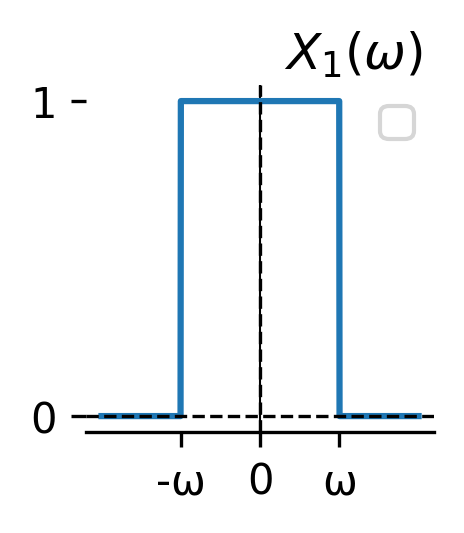
\includegraphics[width=0.4\columnwidth, height=2.5cm]{figs/plot.png}\hfill
    \begin{tabular}{c}
        {\sffamily\raisebox{1.75cm}{*}} 
    \end{tabular}\hfill
    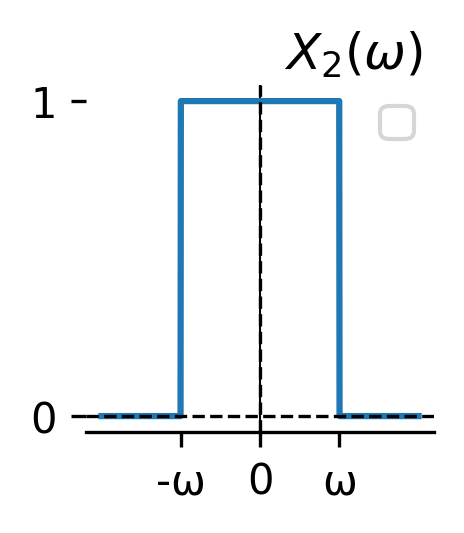
\includegraphics[width=0.4\columnwidth, height=2.5cm]{figs/plot4.png}
    
    \caption{}
    \label{fig:overall}
\end{figure}

\begin{align}
\left(\frac{\sin(\omega t)}{\pi t}\right)^2  \xleftrightarrow{\mathcal{F}} X_3(\omega) 
\end{align}
\begin{figure}[h!]
    \centering
    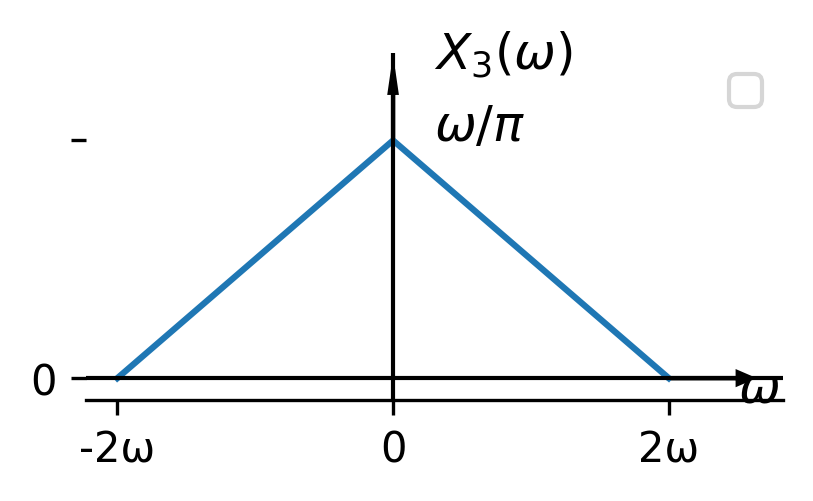
\includegraphics[width=0.5\columnwidth, height=3cm]{figs/plot1.png}
    \caption{}
    \label{fig:sr11}
\end{figure}
\begin{align}
\pi\left(\frac{\sin(\omega t)}{\pi t}\right)^2 \xleftrightarrow{\mathcal{F}} X_4(\omega)
\end{align}
\begin{figure}[h!]
    \centering
    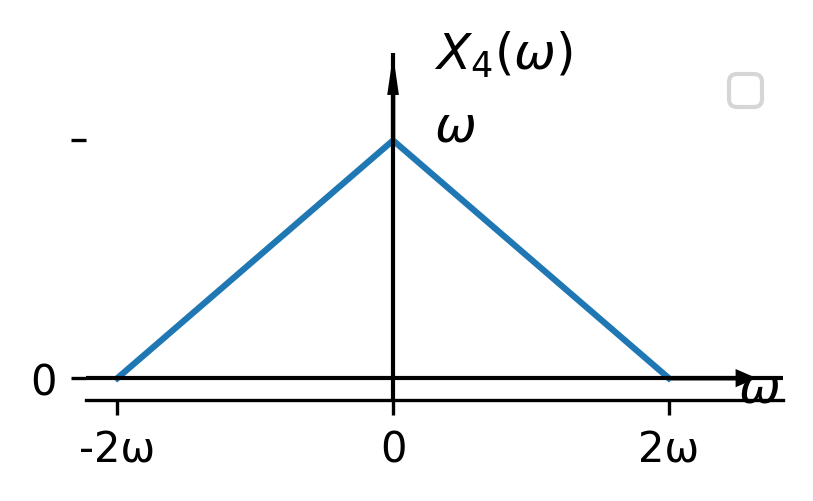
\includegraphics[width=0.5\columnwidth, height=3cm]{figs/plot2.png}
    \caption{}
    \label{fig:sr12}
\end{figure}
    \begin{align}
\text{From modulating property:} \nonumber \\
        f(t) \cos(\omega_0 t) \xleftrightarrow{\mathcal{F}} \frac{1}{2} \left[F(\omega + \omega_0) + F(\omega - \omega_0)\right]
    \end{align}

    \begin{align}
        H(\omega) &= \frac{1}{2} \left[F(\omega + 10\omega) + F(\omega - 10\omega)\right]
    \end{align}

\begin{figure}[h!]
    \centering
    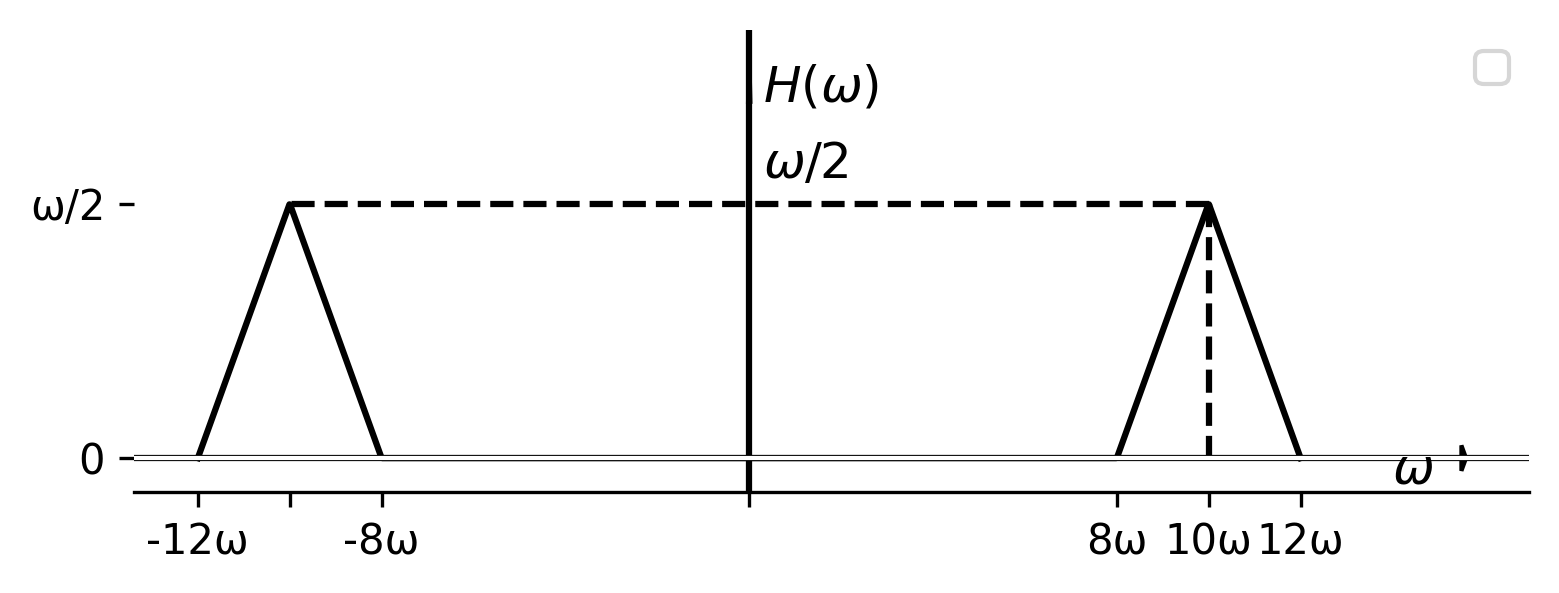
\includegraphics[width=0.7\columnwidth,height=2.5cm]{figs/plot3.png}
    \caption{}
    \label{fig:sr13}
\end{figure}
\begin{equation}
    \frac{\frac{\omega}{2} - 0}{10\omega - 12\omega} = \frac{|H(10.5\omega)| - 0}{10.5\omega - 12\omega}
\end{equation}

\begin{align}
A = |H(10.5\omega)| &= \frac{3}{8}\omega \quad \text{and} \quad  \theta= \angle H(10.5\omega) = 0^\circ
\end{align}

The output \(y(t)\):
\begin{align}
y(t) &= \frac{3}{8}\omega \cdot 10 \cos(10.5 \omega t) \\
&= \frac{15}{4}\omega \cos(10.5 \omega t)
\end{align}
\begin{figure}[h!]
    \centering
    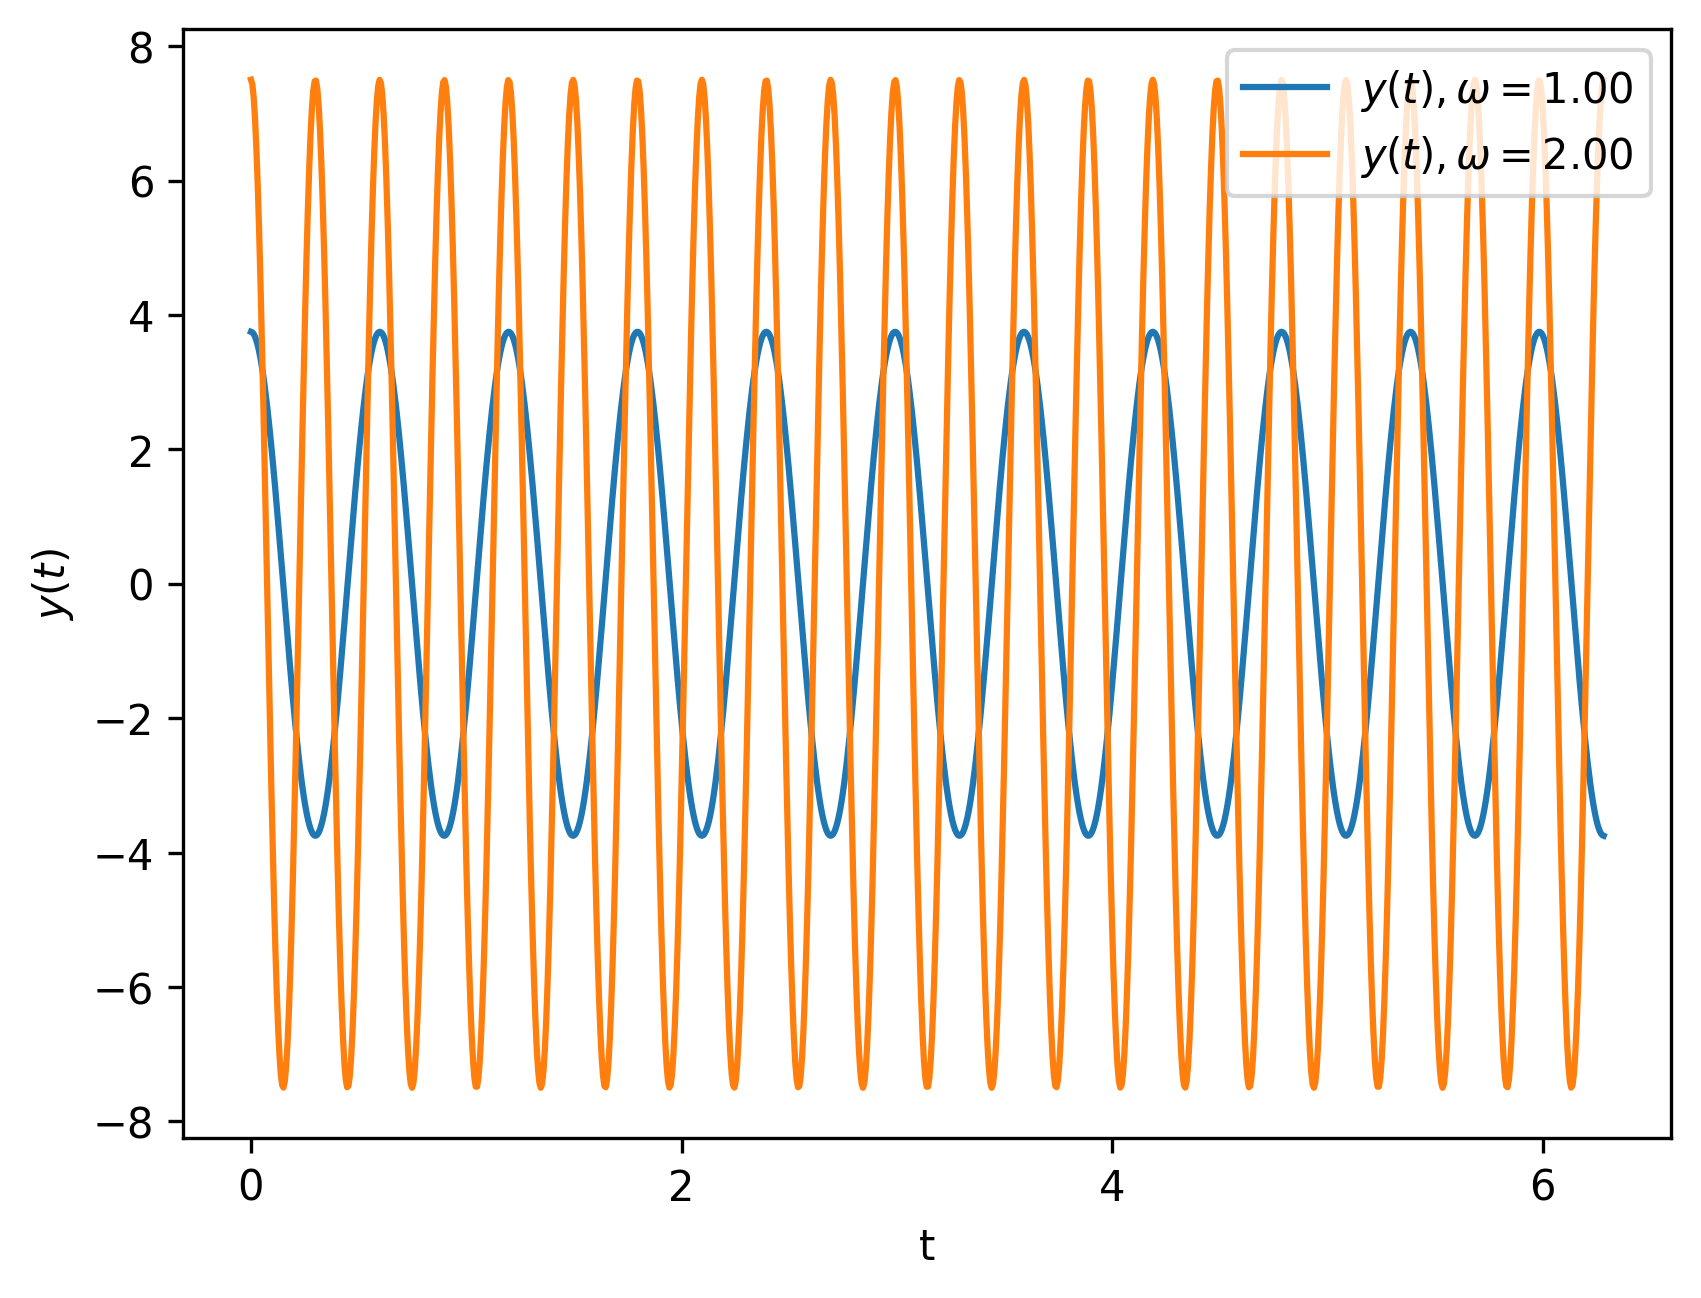
\includegraphics[width=\columnwidth]{figs/plot5.png}
    \caption{}
    \label{fig:sr14}
\end{figure}
\end{document}


\pagebreak

\item The function $f(z)=\frac{1}{z-1}$ of a complex variable z is integrated on a closed contour in an anti-clockwise direction. For which of the following contours, does this integral have a non-zero value?\\
\brak{A}$\abs{z-2}=0.01$\\
\brak{B}$\abs{z-1}=0.1$\\
\brak{C}$\abs{z-3}=5$\\
\brak{D}$\abs{z}=2$\\
\hfill(GATE 2023 BM)\\
\solution
\iffalse
\let\negmedspace\undefined
\let\negthickspace\undefined
\documentclass[journal,12pt,twocolumn]{IEEEtran}
\usepackage{cite}
\usepackage{amsmath,amssymb,amsfonts,amsthm}
\usepackage{algorithmic}
\usepackage{graphicx}
\usepackage{textcomp}
\usepackage{xcolor}
\usepackage{txfonts}
\usepackage{listings}
\usepackage{enumitem}
\usepackage{mathtools}
\usepackage{gensymb}
\usepackage{comment}
\usepackage[breaklinks=true]{hyperref}
\usepackage{tkz-euclide} 
\usepackage{listings}
\usepackage{gvv}                                        
\def\inputGnumericTable{}                                 
\usepackage[latin1]{inputenc}                                
\usepackage{color}                                            
\usepackage{array}                                            
\usepackage{longtable}                              
\usepackage{calc}                                             
\usepackage{multirow}                                         
\usepackage{hhline}                                           
\usepackage{ifthen}                                           
\usepackage{lscape}

\newtheorem{theorem}{Theorem}[section]
\newtheorem{problem}{Problem}
\newtheorem{proposition}{Proposition}[section]
\newtheorem{lemma}{Lemma}[section]
\newtheorem{corollary}[theorem]{Corollary}
\newtheorem{example}{Example}[section]
\newtheorem{definition}[problem]{Definition}
\newcommand{\BEQA}{\begin{eqnarray}}
\newcommand{\EEQA}{\end{eqnarray}}
\newcommand{\define}{\stackrel{\triangle}{=}}
\theoremstyle{remark}
\newtheorem{rem}{Remark}
\begin{document}

\bibliographystyle{IEEEtran}
\vspace{3cm}

\title{GATE 2023}
\author{EE23BTECH11020 - Raghava Ganji$^{*}$% <-this % stops a space
}
\maketitle
\newpage
\bigskip

\renewcommand{\thefigure}{\theenumi}
\renewcommand{\thetable}{\theenumi}

\textbf{GATE 2023 BM.48:}
The function $f(z)=\frac{1}{z-1}$ of a complex variable z on a closed contour in an anti-clockwise direction.For which of the following contours, does this integral have a non-zero value?\\
\brak{A}$\abs{z-2}=0.01$\\
\brak{B}$\abs{z-1}=0.1$\\
\brak{C}$\abs{z-3}=5$\\
\brak{D}$\abs{z}=2$\\
\solution\\
\fi
Cauchy's Integral Formula and Residue Theorem.
\begin{align}
\oint_{c}f\brak z&=2\pi jRes\sbrak{f\brak z,z_0}\label{eq:CIF}\\
Res\sbrak{f\brak z,z_0}&=\lim_{z\to z_0}\sbrak{\brak{z-z_0}f\brak z}\label{eq:Res Thm}
\end{align}
Here $z_0$ is pole of the f\brak z\\
Using \eqref{eq:CIF}
\begin{align}
\oint_{c}\frac{1}{z-1}dz &=2\pi jRes\sbrak{\frac{1}{z-1},1}
\end{align}
\begin{enumerate}
\item For option A the pole is outside the contour, then Residue is zero.\\
\begin{figure}[h!]
    \centering
    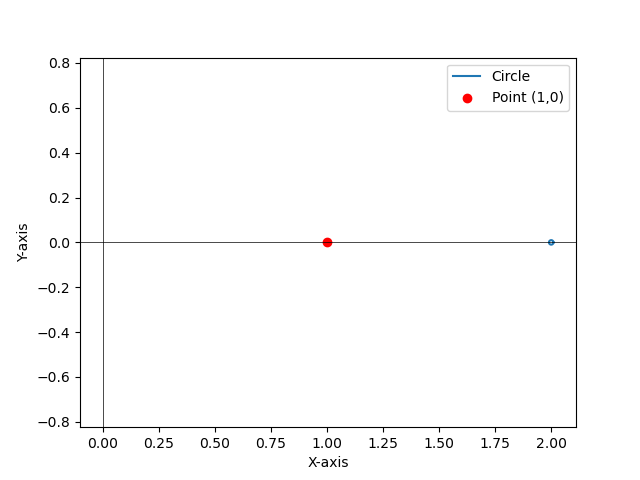
\includegraphics[width=1\columnwidth]{2023/BM/48/figs/plotg231.png}
    \caption{graph of option A}
\end{figure}
\begin{align}
\implies\oint_{c}\frac{1}{z-1}dz &=2\pi j\brak{0}\\
\implies 0
\end{align}
\item For option B the pole is inside the contour.\\
\begin{figure}[h!]
    \centering
    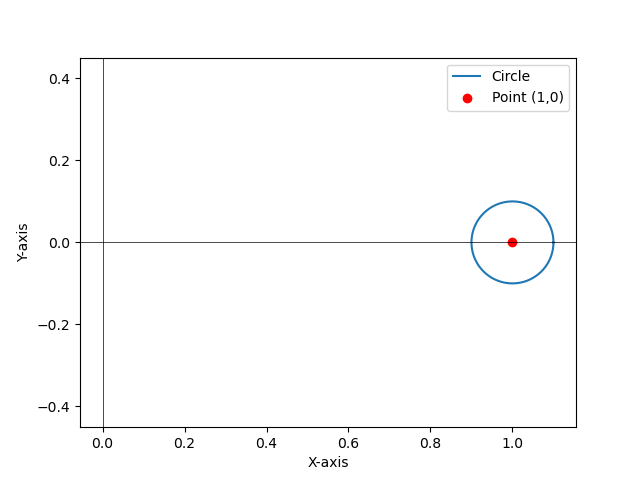
\includegraphics[width=1\columnwidth]{2023/BM/48/figs/plotg232.png}
    \caption{graph of option B}
\end{figure}
Then, using \eqref{eq:Res Thm}
\begin{align}
Res\sbrak{\frac{1}{z-1},1} &=\lim_{z\to 1}\brak{z-1}\frac{1}{z-1}\\
&=1\\
\implies \oint_{c}\frac{1}{z-1}dz&=2\pi j\brak 1\\
\implies 2\pi j
\end{align}
\item For option C the pole is inside the contour.\\
\begin{figure}[h!]
    \centering
    \includegraphics[width=1\columnwidth]{2023/BM/48/figs/plotg233.png}
    \caption{graph of option C}
\end{figure}
Then, using \eqref{eq:Res Thm}
\begin{align}
Res\sbrak{\frac{1}{z-1},1} &=\lim_{z\to 1}\brak{z-1}\frac{1}{z-1}\\
&=1\\
\implies \oint_{c}\frac{1}{z-1}dz&=2\pi j\brak 1\\
\implies 2\pi j
\end{align}
\item For option D the pole is inside the contour.\\
\begin{figure}[h!]
    \centering
    \includegraphics[width=1\columnwidth]{2023/BM/48/figs/plotg234.png}
    \caption{graph of option D}
\end{figure}
Then, using \eqref{eq:Res Thm}
\begin{align}
Res\sbrak{\frac{1}{z-1},1} &=\lim_{z\to 1}\brak{z-1}\frac{1}{z-1}\\
&=1\\
\implies \oint_{c}\frac{1}{z-1}dz&=2\pi j\brak 1\\
\implies 2\pi j
\end{align}
\end{enumerate}
We can conclude that for options B,C,D contours have the non-zero value for this integral.
%\end{document}

\newpage
\item Consider the contour integral $\oint \frac{dz}{z^4 + z^3 - 2z^2}$, along the curve $|z| = 3$ oriented in the counterclockwise direction. If $\text{Res}[f, z_0]$ denotes the residue of $f(z)$ at the point $z_0$, then which of the following are TRUE? \\
\begin{itemize}
    \item (A) $\text{Res}[f, 0] = -\frac{1}{4}$
    \item (B) $\text{Res}[f, 1] = \frac{1}{3}$
    \item (C) $\text{Res}[f, -2] = -\frac{1}{12}$
    \item (D) $\text{Res}[f, 2] = -1$
\end{itemize}
\hfill{(GATE NM 2023)}\\
\solution
\newpage
\end{enumerate}

\chapter{Laplace Transform}
 \begin{enumerate}[label=\thechapter.\arabic*,ref=\thechapter.\theenumi]

\item The number of zeroes of the polynomial $P(s) = s^3+2s^2+5s+80$ in the right side of the plane?\hfill(GATE IN 2023) \\

\solution
\iffalse
\let\negmedspace\undefined
\let\negthickspace\undefined
\documentclass[journal,12pt,twocolumn]{IEEEtran}
\usepackage{cite}
\usepackage{amsmath,amssymb,amsfonts}
\usepackage{graphicx}
\usepackage{textcomp}
\usepackage{xcolor}
\usepackage{txfonts}
\usepackage{listings}
\usepackage{enumitem}
\usepackage{mathtools}
\usepackage{gensymb}
\usepackage{comment}
\usepackage[breaklinks=true]{hyperref}
\usepackage{tkz-euclide} 
\usepackage{listings}
\usepackage{gvv}                                        
\def\inputGnumericTable{}                                 
\usepackage[latin1]{inputenc}                                
\usepackage{color}                                            
\usepackage{array}                                            
\usepackage{longtable}                                       
\usepackage{calc}                                             
\usepackage{multirow}                                         
\usepackage{hhline}                                           
\usepackage{ifthen}                                           
\usepackage{lscape}
\usepackage[export]{adjustbox}

\newtheorem{theorem}{Theorem}[section]
\newtheorem{problem}{Problem}
\newtheorem{proposition}{Proposition}[section]
\newtheorem{lemma}{Lemma}[section]
\newtheorem{corollary}[theorem]{Corollary}
\newtheorem{example}{Example}[section]
\newtheorem{definition}[problem]{Definition}
\newcommand{\BEQA}{\begin{eqnarray}}
\newcommand{\EEQA}{\end{eqnarray}}
\newcommand{\define}{\stackrel{\triangle}{=}}
\newtheorem{rem}{Remark}

\begin{document}
\parindent 0px
\bibliographystyle{IEEEtran}

\vspace{3cm}

\title{}
\author{EE23BTECH11042 -  Khusinadha Naik$^{*}$
}
\maketitle
\newpage
\bigskip

% \renewcommand{\thefigure}{\theenumi}
% \renewcommand{\thetable}{\theenumi}


\noindent \textbf{26.} \hspace{2pt}A causal, discrete time system is described by the difference equation $y[n] = 0.5 y[n-1] + x[n]$, for all $n$, where $y[n]$ denotes the output sequence and $x[n]$ denotes the input sequence. Which of the following statements is/are TRUE?
\begin{flushright}
\hfill(GATE 2023 BM)
\end{flushright}
\begin{enumerate}[label = (\alph*)]
	\item The system has an impulse response described by $0.5^{n} u[-n]$ where $u[n]$ is the  
unit step sequence. 	\label{option:GATE.2023.BM.26.1}	
	\item The system is stable in the bounded input, bounded output sense.		\label{option:GATE.2023.BM.26.2}
	\item The system has an infinite number of non-zero samples in its impulse response	\label{option:GATE.2023.BM.26.3}
	\item The system has a finite number of non-zero samples in its impulse response.	\label{option:GATE.2023.BM.26.4}
\end{enumerate}

\noindent \textbf{Ans.}\\
\fi
\begin{table}[h]
\centering
\begin{tabular}{|c|c|c|}
        \hline
        \textbf{Parameter} & \textbf{Value} & \textbf{Description} \\
        \hline
        $x[n]$ & ? & Input Sequence \\
        \hline
        $y[n]$ & ? & Output Sequence \\
        \hline
\end{tabular}
\caption{Input parameters table}
\label{tab:GATE.2023.BM.26.1}





\end{table}
\begin{align}
y[n] = 0.5y[n-1] + x[n] 
\end{align}

Taking $Z$-Transform 
\begin{align}
Y\brak{z} &= 0.5z^{-1}Y\brak{z} + X\brak{z} \\
\implies \frac{Y\brak{z}}{X\brak{z}} &= \frac{1}{1 - 0.5z^{-1}} = H\brak{z} 
\end{align}
If $x[n]$ is impulse input 
\begin{align}
\implies &Y\brak{z} = H\brak{z} = \frac{1}{1 - 0.5z^{-1}}  \label{eq:GATE.2023.BM.26.4}
\end{align}
From \eqref{eq:GATE.2023.BM.26.4} pole lies at $z = 0.5$
\begin{align}
a^{n}u\brak{n} \xleftrightarrow{\mathcal{Z}} &\frac{1}{1 - az^{-1}} \quad , \abs{z} > a \label{eq:GATE.2023.BM.26.5}
\end{align}

From \eqref{eq:GATE.2023.BM.26.4} , \eqref{eq:GATE.2023.BM.26.5}
\begin{align}
h[n] = 0.5^{n}u[n] \quad , \abs{z} > 0.5 \label{eq:GATE.2023.BM.26.6}
\end{align}


\pagebreak
Plotting $h[n]$ vs $n$
\begin{figure}[h]
    \includegraphics[width=0.5\textwidth]{2023/BM/26/figs/fig1.png}
    \caption{Plot of $h[n]$ vs $n$}
    \label{fig:GATE.2023.BM.26.1}
\end{figure}

\begin{enumerate}
\item From \eqref{eq:GATE.2023.BM.26.6} , \ref{option:GATE.2023.BM.26.1} is wrong
\item As pole lies within unit circle \ref{option:GATE.2023.BM.26.2} is true
\item From \eqref{eq:GATE.2023.BM.26.6} and \figref{fig:GATE.2023.BM.26.1} ,\ref{option:GATE.2023.BM.26.3} is true and hence
\item \ref{option:GATE.2023.BM.26.4} is false 
\end{enumerate}





%\end{document}

\newpage

\item The circuit shown in the figure is initially in the steady state with the switch K in open condition and $\overline{K}$ in closed condition. The switch K is closed and $\overline{K}$ is opened simultaneously at the instant $t = t_1$, where $t_1 > 0$. The minimum value of $t_1$ in milliseconds such that there is no transient in the voltage across the 100 $\mu F$ capacitor, is \rule{1cm}{0.15mm} (Round off to 2 decimal places) \hfill (GATE EE 2023)
\begin{circuitikz}
     \draw (0,0) node[left] {$x_1(t)$} to (0.8,0);
     \draw (0,-1) node[left] {$x_2(t)$} to (0.8,-1);
     \draw (1,0) circle(0.2);
     \draw (1,0) node {$\times$};
     \draw (1,-1) circle(0.2);
     \draw (1,-1) node {$\times$};
    \draw (1.2,0) to (1.8,0);
    \draw (1.2,-1) to (1.8,-1);
    \draw (1.8,0) to (1.8,-0.3);
    \draw (1.8,-1) to (1.8,-0.7);
    \draw (1.8,-0.5) circle(0.2);
    \draw (1.8,-0.5) node {$+$};
    \draw[->] (1,0.5) to (1,0.2) ;
    \node at (1,0.6) {cos$(4\pi\times10^3t)$};
    \draw[->] (1,-1.5) to (1,-1.2);
    \node at (1,-1.6) {cos$(12\pi\times10^3t)$};
    \draw (2,-0.5) to (2.3,-0.5);
    \node at (2.6,-0.5) {y(t)};
     
     
\end{circuitikz}
\\
\solution
\iffalse
\let\negmedspace\undefined
\let\negthickspace\undefined
\documentclass[journal,12pt,twocolumn]{IEEEtran}
\usepackage{cite}
\usepackage{amsmath,amssymb,amsfonts}
\usepackage{graphicx}
\usepackage{textcomp}
\usepackage{xcolor}
\usepackage{txfonts}
\usepackage{listings}
\usepackage{enumitem}
\usepackage{mathtools}
\usepackage{gensymb}
\usepackage{comment}
\usepackage[breaklinks=true]{hyperref}
\usepackage{tkz-euclide} 
\usepackage{listings}
\usepackage{gvv}                                        
\def\inputGnumericTable{}                                 
\usepackage[latin1]{inputenc}                                
\usepackage{color}                                            
\usepackage{array}                                            
\usepackage{longtable}                                       
\usepackage{calc}                                             
\usepackage{multirow}                                         
\usepackage{hhline}                                           
\usepackage{ifthen}                                           
\usepackage{lscape}
\usepackage[export]{adjustbox}

\newtheorem{theorem}{Theorem}[section]
\newtheorem{problem}{Problem}
\newtheorem{proposition}{Proposition}[section]
\newtheorem{lemma}{Lemma}[section]
\newtheorem{corollary}[theorem]{Corollary}
\newtheorem{example}{Example}[section]
\newtheorem{definition}[problem]{Definition}
\newcommand{\BEQA}{\begin{eqnarray}}
\newcommand{\EEQA}{\end{eqnarray}}
\newcommand{\define}{\stackrel{\triangle}{=}}
\newtheorem{rem}{Remark}

\begin{document}
\parindent 0px
\bibliographystyle{IEEEtran}

\vspace{3cm}

\title{}
\author{EE23BTECH11042 -  Khusinadha Naik$^{*}$
}
\maketitle
\newpage
\bigskip

% \renewcommand{\thefigure}{\theenumi}
% \renewcommand{\thetable}{\theenumi}


\noindent \textbf{26.} \hspace{2pt}A causal, discrete time system is described by the difference equation $y[n] = 0.5 y[n-1] + x[n]$, for all $n$, where $y[n]$ denotes the output sequence and $x[n]$ denotes the input sequence. Which of the following statements is/are TRUE?
\begin{flushright}
\hfill(GATE 2023 BM)
\end{flushright}
\begin{enumerate}[label = (\alph*)]
	\item The system has an impulse response described by $0.5^{n} u[-n]$ where $u[n]$ is the  
unit step sequence. 	\label{option:GATE.2023.BM.26.1}	
	\item The system is stable in the bounded input, bounded output sense.		\label{option:GATE.2023.BM.26.2}
	\item The system has an infinite number of non-zero samples in its impulse response	\label{option:GATE.2023.BM.26.3}
	\item The system has a finite number of non-zero samples in its impulse response.	\label{option:GATE.2023.BM.26.4}
\end{enumerate}

\noindent \textbf{Ans.}\\
\fi
\begin{table}[h]
\centering
\begin{tabular}{|c|c|c|}
        \hline
        \textbf{Parameter} & \textbf{Value} & \textbf{Description} \\
        \hline
        $x[n]$ & ? & Input Sequence \\
        \hline
        $y[n]$ & ? & Output Sequence \\
        \hline
\end{tabular}
\caption{Input parameters table}
\label{tab:GATE.2023.BM.26.1}





\end{table}
\begin{align}
y[n] = 0.5y[n-1] + x[n] 
\end{align}

Taking $Z$-Transform 
\begin{align}
Y\brak{z} &= 0.5z^{-1}Y\brak{z} + X\brak{z} \\
\implies \frac{Y\brak{z}}{X\brak{z}} &= \frac{1}{1 - 0.5z^{-1}} = H\brak{z} 
\end{align}
If $x[n]$ is impulse input 
\begin{align}
\implies &Y\brak{z} = H\brak{z} = \frac{1}{1 - 0.5z^{-1}}  \label{eq:GATE.2023.BM.26.4}
\end{align}
From \eqref{eq:GATE.2023.BM.26.4} pole lies at $z = 0.5$
\begin{align}
a^{n}u\brak{n} \xleftrightarrow{\mathcal{Z}} &\frac{1}{1 - az^{-1}} \quad , \abs{z} > a \label{eq:GATE.2023.BM.26.5}
\end{align}

From \eqref{eq:GATE.2023.BM.26.4} , \eqref{eq:GATE.2023.BM.26.5}
\begin{align}
h[n] = 0.5^{n}u[n] \quad , \abs{z} > 0.5 \label{eq:GATE.2023.BM.26.6}
\end{align}


\pagebreak
Plotting $h[n]$ vs $n$
\begin{figure}[h]
    \includegraphics[width=0.5\textwidth]{2023/BM/26/figs/fig1.png}
    \caption{Plot of $h[n]$ vs $n$}
    \label{fig:GATE.2023.BM.26.1}
\end{figure}

\begin{enumerate}
\item From \eqref{eq:GATE.2023.BM.26.6} , \ref{option:GATE.2023.BM.26.1} is wrong
\item As pole lies within unit circle \ref{option:GATE.2023.BM.26.2} is true
\item From \eqref{eq:GATE.2023.BM.26.6} and \figref{fig:GATE.2023.BM.26.1} ,\ref{option:GATE.2023.BM.26.3} is true and hence
\item \ref{option:GATE.2023.BM.26.4} is false 
\end{enumerate}





%\end{document}


\newpage
\item $y=e^{mx}+e^{-mx}$ is the solution of which differential equation?
\begin{enumerate}[label=\textbf{\arabic*.}, font=\bfseries, align=left]
    \item $\frac{dy}{dx} - my = 0$ 
    \item $\frac{dy}{dx} + my = 0$ 
    \item $\frac{d^{2}y}{dx^{2}} + m^{2}y = 0$ 
    \item $\frac{d^{2}y}{dx^{2}} - m^{2}y = 0$ 
\end{enumerate} \hfill(GATE AG 2023)
\solution

\newpage
\item  A cascade control strategy is shown in the figure below. The transfer function between the output $(y)$ and the secondary disturbance $(d_2)$ is defined as  \\
$$G_{d2}(s)= \frac{y(s)}{d_2(s)}$$. 
Which one of the following is the CORRECT expression for the transfer function $G_{d2}(s)$? \\
\begin{figure}[h]
    \centering
    \includegraphics[scale=0.25]{2023/CH/44/figs/g44fig1.jpeg}
    \caption{ }
    \label{}
\end{figure}
\begin{enumerate}[label=\Alph*.]
\item $\frac{1}{(11s+21)(0.1s+1)}$ 
\item $\frac{1}{(s+1)(0.1s+1)}$
\item $\frac{(s+1)}{(s+2)(0.1s+1)}$
\item $\frac{(s+1)}{(s+1)(0.1s+1)}$
\end{enumerate} \hfill (GATE CH 2023)
\solution
\input{2023/CH/44/g44.1.tex}
\newpage
\item In the differential equation $\frac{dy}{dx} + \alpha x y = 0, \alpha$ is a positive constant. If $y = 1.0$ at
$x = 0.0$, and $y = 0.8$ at $x = 1.0$, the value of $\alpha$ is (rounded off to three decimal places).  \hfill(GATE CE 2023)
\solution

\newpage
\item The switch $S_1$ was closed and $S_2$ was open for a long time. At t=0,switch $S_1$ is opened and $S_2$ is closed,simultaneously. The value of $i_c(0^{+})$, in amperes, is  \hfill (GATE EC 44)\\
\begin{circuitikz}
     \draw (0,0) node[left] {$x_1(t)$} to (0.8,0);
     \draw (0,-1) node[left] {$x_2(t)$} to (0.8,-1);
     \draw (1,0) circle(0.2);
     \draw (1,0) node {$\times$};
     \draw (1,-1) circle(0.2);
     \draw (1,-1) node {$\times$};
    \draw (1.2,0) to (1.8,0);
    \draw (1.2,-1) to (1.8,-1);
    \draw (1.8,0) to (1.8,-0.3);
    \draw (1.8,-1) to (1.8,-0.7);
    \draw (1.8,-0.5) circle(0.2);
    \draw (1.8,-0.5) node {$+$};
    \draw[->] (1,0.5) to (1,0.2) ;
    \node at (1,0.6) {cos$(4\pi\times10^3t)$};
    \draw[->] (1,-1.5) to (1,-1.2);
    \node at (1,-1.6) {cos$(12\pi\times10^3t)$};
    \draw (2,-0.5) to (2.3,-0.5);
    \node at (2.6,-0.5) {y(t)};
     
     
\end{circuitikz}
\\
\solution \\
\documentclass[journal,12pt,twocolumn]{IEEEtran}

% Packages
\usepackage{cite}
\usepackage{amsmath,amssymb,amsfonts,amsthm}
\usepackage{graphicx}
\usepackage{textcomp}
\usepackage{xcolor}
\usepackage{txfonts}
\usepackage{listings}
\usepackage{enumitem}
\usepackage{mathtools}
\usepackage{float}
\usepackage{gensymb}
\usepackage{comment}
\usepackage{hyperref}
\usepackage{tkz-euclide}
\usepackage{gvv}
\usepackage[latin1]{inputenc}
\usepackage{color}
\usepackage{array}
\usepackage{longtable}
\usepackage{calc}
\usepackage{multirow}
\usepackage{hhline}
\usepackage{ifthen}
\usepackage{lscape}
\usepackage{subcaption}
\usepackage{tikz}
\usepackage{circuitikz}
\usepackage{wrapfig}
\usepackage{lipsum}
\usepackage[export]{adjustbox}
\usepackage{inputenc}

% Custom commands and macros
\newtheorem{theorem}{Theorem}[section]
\newtheorem{problem}{Problem}
\newtheorem{proposition}{Proposition}[section]
\newtheorem{lemma}{Lemma}[section]
\newtheorem{corollary}[theorem]{Corollary}
\newtheorem{example}{Example}[section]
\newtheorem{definition}[problem]{Definition}
\newtheorem{rem}{Remark}
\newcommand{\BEQA}{\begin{eqnarray}}
\newcommand{\EEQA}{\end{eqnarray}}
\newcommand{\define}{\stackrel{\triangle}{=}}
\renewcommand{\thefigure}{\theenumi}
\renewcommand{\thetable}{\theenumi}



\begin{document}

\title{GATE 2023 EC 49}
\author{EE23BTECH11045 - Palavelli Srija$^{*}$}
\maketitle

\bigskip

\textbf{Question 12.7.7:} 
Let $x(t) = 10 \cos(10.5 \omega t)$ be passed through an LTI system with impulse response $h(t) = \pi\left(\frac{\sin(\omega t)}{\pi t}\right)^2 \cos(10 \omega t)$ . The output of the system is: \\

\textbf{Solution:}
\begin{table}[h!]
    \centering
    \begin{table}[htbp]
	\centering
	\noindent
	\fontsize{10}{15}\selectfont {
		\resizebox{0.45\textwidth}{!}{%
			\begin{tabular}{|c|c|c|}
				\hline
				\textbf{Parameter} & \textbf{Value} & \textbf{Description} \\
				\hline
				$x\brak t$ & - & Input voltage \\
				\hline
				$y\brak t$ & - & Output voltage \\
				\hline
				$h\brak t$ & $\frac{y\brak t}{x\brak t}$ & Impulse response \\
				\hline
				$X\brak s$ & - & Input voltage in s-domain \\
				\hline
				$Y\brak s$ & - & Output voltage in s-domain \\
				\hline
				$H\brak s$ & $\frac{Y\brak s}{X\brak s}$ & Impulse response in s-domain \\
				\hline
			\end{tabular}
	} }
	\caption*{Input Table}
	
\end{table}
    \caption{Input Parameters}
    \label{tab:table_sr10}
\end{table}

Given \(h(t)\) is real and even. When a sinusoidal input is applied to an LTI system with an even impulse response, the output will also be sinusoidal. Hence, \(y(t) = A\cdot 10\cos(10.5 \omega t + \theta)\).

\[
x(t) \xrightarrow{\text{}} \boxed{\text{h(t)}} \xrightarrow{\text{}} y(t)
\]

\begin{align}
\text{Let } f(t) &= \pi\left(\frac{\sin(\omega t)}{\pi t}\right)^2 \\
h(t) &= f(t) \cos(10 \omega t)
\end{align}

Using 
\begin{align}
x_1(t) \cdot x_2(t) \xleftrightarrow{\mathcal{F}} X_1(\omega) * X_2(\omega)\\
\left(\frac{\sin(\omega t)}{\pi t}\right) \cdot \left(\frac{\sin(\omega t)}{\pi t}\right) \xleftrightarrow{\mathcal{F}} X_1(\omega) * X_2(\omega)
\end{align}
\begin{figure}[h!]
    \centering
    \includegraphics[width=0.4\columnwidth, height=2.5cm]{figs/plot.png}\hfill
    \begin{tabular}{c}
        {\sffamily\raisebox{1.75cm}{*}} 
    \end{tabular}\hfill
    \includegraphics[width=0.4\columnwidth, height=2.5cm]{figs/plot4.png}
    
    \caption{}
    \label{fig:overall}
\end{figure}

\begin{align}
\left(\frac{\sin(\omega t)}{\pi t}\right)^2  \xleftrightarrow{\mathcal{F}} X_3(\omega) 
\end{align}
\begin{figure}[h!]
    \centering
    \includegraphics[width=0.5\columnwidth, height=3cm]{figs/plot1.png}
    \caption{}
    \label{fig:sr11}
\end{figure}
\begin{align}
\pi\left(\frac{\sin(\omega t)}{\pi t}\right)^2 \xleftrightarrow{\mathcal{F}} X_4(\omega)
\end{align}
\begin{figure}[h!]
    \centering
    \includegraphics[width=0.5\columnwidth, height=3cm]{figs/plot2.png}
    \caption{}
    \label{fig:sr12}
\end{figure}
    \begin{align}
\text{From modulating property:} \nonumber \\
        f(t) \cos(\omega_0 t) \xleftrightarrow{\mathcal{F}} \frac{1}{2} \left[F(\omega + \omega_0) + F(\omega - \omega_0)\right]
    \end{align}

    \begin{align}
        H(\omega) &= \frac{1}{2} \left[F(\omega + 10\omega) + F(\omega - 10\omega)\right]
    \end{align}

\begin{figure}[h!]
    \centering
    \includegraphics[width=0.7\columnwidth,height=2.5cm]{figs/plot3.png}
    \caption{}
    \label{fig:sr13}
\end{figure}
\begin{equation}
    \frac{\frac{\omega}{2} - 0}{10\omega - 12\omega} = \frac{|H(10.5\omega)| - 0}{10.5\omega - 12\omega}
\end{equation}

\begin{align}
A = |H(10.5\omega)| &= \frac{3}{8}\omega \quad \text{and} \quad  \theta= \angle H(10.5\omega) = 0^\circ
\end{align}

The output \(y(t)\):
\begin{align}
y(t) &= \frac{3}{8}\omega \cdot 10 \cos(10.5 \omega t) \\
&= \frac{15}{4}\omega \cos(10.5 \omega t)
\end{align}
\begin{figure}[h!]
    \centering
    \includegraphics[width=\columnwidth]{figs/plot5.png}
    \caption{}
    \label{fig:sr14}
\end{figure}
\end{document}


\newpage

\item The continuous time signal $x(t)$ is described by:
\begin{align}
x(t)=
    \begin{cases}
        1, & \text{if } 0\: {\displaystyle \leq }\:t\:{\displaystyle \leq }\:1\\
        0, & \text{elsewhere}
    \end{cases} 
\end{align}
If $y(t)$ represents $x(t)$ convolved with itself, which of the following options is/are TRUE?
\begin{enumerate}[label = \Alph*]
    \item $y(t)$ = 0 for all $t<0$\\
    \item $y(t)$ = 0 for all $t>1$\\
    \item $y(t)$ = 0 for all $t>3$\\
    \item $\int_{0.1}^{0.75} \frac{dy(t)}{dt}\: \text{dt} \neq 0$
\end{enumerate}
\solution
\newpage

\item The Z-transform of a discrete signal $x\brak{n}$ is
\begin{align}
X\brak{z}=\dfrac{4z}{\brak{z-\dfrac{1}{5}} \brak{z-\dfrac{2}{3}} \brak{z-3}} \text{ with ROC= }R
\end{align}
Which one of the following statements is TRUE?
\begin{enumerate}[label = (\alph*)]
     \item Discrete time Fourier transform of $x\sbrak{n}$ converges if $R$ is $|z|>3$\\
     \item Discrete time Fourier transform of $x\sbrak{n}$ converges if $ R$ is $\dfrac{2}{3}<|z|<3$\\
     \item Discrete time Fourier transform of $x\sbrak{n}$ converges if $R$ is such that $x\sbrak{n}$ is a left-sided sequence.\\
     \item Discrete time Fourier transform of $x\sbrak{n}$ converges if $R$ is such that $x\sbrak{n}$is a right-sided sequence.\\
 \end{enumerate} \hfill{GATE EE 2023}	\\
 \solution
 \input{2023/EE/19/1.tex}
 \newpage
 
\item The phase margin of the transfer function $G(s) = \frac{2(1-s)}{(1+s)^2}$ is \rule{1cm}{0.15mm} degrees. (rounded off to the nearest integer). \hfill (GATE IN 2023)\\
\solution
\input{2023/IN/50/in_50.tex}
\newpage
\item Consider the second-order linear differential equation
\[x^2\frac{d^2y}{dx^2}+x\frac{dy}{dx}-y=0, \; x\geq 1\]
with the initial conditions \[y(x=1)=6,\; \;\; \frac{dy}{dx}\big{|}_{x=1}=2.\]
Then the value of $y$ at $x=2$ is \rule{2cm}{0.1mm}.\\{\hfill{GATE ME 2023}}\\
\solution
\iffalse
\let\negmedspace\undefined
\let\negthickspace\undefined
\documentclass[journal,12pt,twocolumn]{IEEEtran}
\usepackage{cite}
\usepackage{amsmath,amssymb,amsfonts}
\usepackage{graphicx}
\usepackage{textcomp}
\usepackage{xcolor}
\usepackage{txfonts}
\usepackage{listings}
\usepackage{enumitem}
\usepackage{mathtools}
\usepackage{gensymb}
\usepackage{comment}
\usepackage[breaklinks=true]{hyperref}
\usepackage{tkz-euclide} 
\usepackage{listings}
\usepackage{gvv}                                        
\def\inputGnumericTable{}                                 
\usepackage[latin1]{inputenc}                                
\usepackage{color}                                            
\usepackage{array}                                            
\usepackage{longtable}                                       
\usepackage{calc}                                             
\usepackage{multirow}                                         
\usepackage{hhline}                                           
\usepackage{ifthen}                                           
\usepackage{lscape}
\usepackage[export]{adjustbox}

\newtheorem{theorem}{Theorem}[section]
\newtheorem{problem}{Problem}
\newtheorem{proposition}{Proposition}[section]
\newtheorem{lemma}{Lemma}[section]
\newtheorem{corollary}[theorem]{Corollary}
\newtheorem{example}{Example}[section]
\newtheorem{definition}[problem]{Definition}
\newcommand{\BEQA}{\begin{eqnarray}}
\newcommand{\EEQA}{\end{eqnarray}}
\newcommand{\define}{\stackrel{\triangle}{=}}
\newtheorem{rem}{Remark}

\begin{document}
\parindent 0px
\bibliographystyle{IEEEtran}

\vspace{3cm}

\title{}
\author{EE23BTECH11042 -  Khusinadha Naik$^{*}$
}
\maketitle
\newpage
\bigskip

% \renewcommand{\thefigure}{\theenumi}
% \renewcommand{\thetable}{\theenumi}


\noindent \textbf{26.} \hspace{2pt}A causal, discrete time system is described by the difference equation $y[n] = 0.5 y[n-1] + x[n]$, for all $n$, where $y[n]$ denotes the output sequence and $x[n]$ denotes the input sequence. Which of the following statements is/are TRUE?
\begin{flushright}
\hfill(GATE 2023 BM)
\end{flushright}
\begin{enumerate}[label = (\alph*)]
	\item The system has an impulse response described by $0.5^{n} u[-n]$ where $u[n]$ is the  
unit step sequence. 	\label{option:GATE.2023.BM.26.1}	
	\item The system is stable in the bounded input, bounded output sense.		\label{option:GATE.2023.BM.26.2}
	\item The system has an infinite number of non-zero samples in its impulse response	\label{option:GATE.2023.BM.26.3}
	\item The system has a finite number of non-zero samples in its impulse response.	\label{option:GATE.2023.BM.26.4}
\end{enumerate}

\noindent \textbf{Ans.}\\
\fi
\begin{table}[h]
\centering
\begin{tabular}{|c|c|c|}
        \hline
        \textbf{Parameter} & \textbf{Value} & \textbf{Description} \\
        \hline
        $x[n]$ & ? & Input Sequence \\
        \hline
        $y[n]$ & ? & Output Sequence \\
        \hline
\end{tabular}
\caption{Input parameters table}
\label{tab:GATE.2023.BM.26.1}





\end{table}
\begin{align}
y[n] = 0.5y[n-1] + x[n] 
\end{align}

Taking $Z$-Transform 
\begin{align}
Y\brak{z} &= 0.5z^{-1}Y\brak{z} + X\brak{z} \\
\implies \frac{Y\brak{z}}{X\brak{z}} &= \frac{1}{1 - 0.5z^{-1}} = H\brak{z} 
\end{align}
If $x[n]$ is impulse input 
\begin{align}
\implies &Y\brak{z} = H\brak{z} = \frac{1}{1 - 0.5z^{-1}}  \label{eq:GATE.2023.BM.26.4}
\end{align}
From \eqref{eq:GATE.2023.BM.26.4} pole lies at $z = 0.5$
\begin{align}
a^{n}u\brak{n} \xleftrightarrow{\mathcal{Z}} &\frac{1}{1 - az^{-1}} \quad , \abs{z} > a \label{eq:GATE.2023.BM.26.5}
\end{align}

From \eqref{eq:GATE.2023.BM.26.4} , \eqref{eq:GATE.2023.BM.26.5}
\begin{align}
h[n] = 0.5^{n}u[n] \quad , \abs{z} > 0.5 \label{eq:GATE.2023.BM.26.6}
\end{align}


\pagebreak
Plotting $h[n]$ vs $n$
\begin{figure}[h]
    \includegraphics[width=0.5\textwidth]{2023/BM/26/figs/fig1.png}
    \caption{Plot of $h[n]$ vs $n$}
    \label{fig:GATE.2023.BM.26.1}
\end{figure}

\begin{enumerate}
\item From \eqref{eq:GATE.2023.BM.26.6} , \ref{option:GATE.2023.BM.26.1} is wrong
\item As pole lies within unit circle \ref{option:GATE.2023.BM.26.2} is true
\item From \eqref{eq:GATE.2023.BM.26.6} and \figref{fig:GATE.2023.BM.26.1} ,\ref{option:GATE.2023.BM.26.3} is true and hence
\item \ref{option:GATE.2023.BM.26.4} is false 
\end{enumerate}





%\end{document}

\newpage
\item The transfer function of a measuring instrument is \\
$$G_m(s) = \frac{1.05}{2s+1}exp(-s)$$
At time $t = 0$, a step change of +1 unit is introduced in the input of this instrument.The time taken by the instrument to show an increase of 1 unit in its output is(rounded off to two decimal places).\\ \hfill (GATE CH 2023)
\solution
\item
The laplace transform of $x_1(t)$ = $e^{-t}u(t)$ is $X_1(s)$, where $u(t)$ is the unit step function. The laplace transform of $x_2(t) = e^tu(-t)$ is $X_2(s)$. Which one of the following statements is TRUE?
\begin{enumerate}
    \item The region of convergence of $X_1(s)$ is $Re(s) \geq 0$
    \item The region of convergence of $X_2(s)$ is confined to the left half-plane of s.
    \item The region of convergence of $X_1(s)$ is confined to the right half-plane of s.
    \item the imaginary axis in the s-plane is included in both the region of convergence of $X_1(s)$ and the region of convergence of $X_2(s)$.
\end{enumerate} \hfill(GATE BM 2023)\\
\solution
\input{2023/BM/39/bm39.tex}
\newpage
\item Given that $\frac{dy}{dx}=2x+y$ and $y=1$,when $x=0$ Using Runge-Kutta fourth order method,the value of $y$ at $x=0.2$ is \hfill(GATE 2023 AG 50) \\
\solution

\item The magnitude and phase plots shown in the figure match with the transfer-
function
\begin{figure}[h]
    \centering
    \includegraphics[width=\columnwidth]{2023/IN/43/figs/question.png}
\end{figure}\\
\begin{enumerate}
\item $\frac{10000}{s^2+2s+10000}$\\
\item $\frac{10000}{s^2+2s+10000}e^{-0.05s}$\\
\item $\frac{10000}{s^2+2s+10000}e^{-0.5\times10^{-12}s}$\\
\item $\frac{100}{s^2+2s+100}$
\end{enumerate}
\hfill{(GATE IN 2023)}
\solution

\newpage
\item The Laplace transform of the continuous-time signal $x\brak{t} = e^{-3t}u\brak{t - 5}$ is 
\rule{1cm}{0.15mm}, where $u\brak{t}$ denotes the continuous-time unit step signal.

\begin{enumerate}[label = \Alph*)]
    \item $\frac{e^{-5s}}{s + 3}$, Real$\{s\} > -3$\\
    \item $\frac{e^{-5(s - 3)}}{s - 3}$, Real$\{s\} > 3$\\
    \item $\frac{e^{-5(s + 3)}}{s + 3}$, Real$\{s\} > -3$\\
    \item $\frac{e^{-5(s - 3)}}{s + 3}$, Real$\{s\} > -3$\\
\end{enumerate}
\solution
\iffalse
\let\negmedspace\undefined
\let\negthickspace\undefined
\documentclass[journal,12pt,twocolumn]{IEEEtran}
\usepackage{cite}
\usepackage{amsmath,amssymb,amsfonts}
\usepackage{graphicx}
\usepackage{textcomp}
\usepackage{xcolor}
\usepackage{txfonts}
\usepackage{listings}
\usepackage{enumitem}
\usepackage{mathtools}
\usepackage{gensymb}
\usepackage{comment}
\usepackage[breaklinks=true]{hyperref}
\usepackage{tkz-euclide} 
\usepackage{listings}
\usepackage{gvv}                                        
\def\inputGnumericTable{}                                 
\usepackage[latin1]{inputenc}                                
\usepackage{color}                                            
\usepackage{array}                                            
\usepackage{longtable}                                       
\usepackage{calc}                                             
\usepackage{multirow}                                         
\usepackage{hhline}                                           
\usepackage{ifthen}                                           
\usepackage{lscape}
\usepackage[export]{adjustbox}

\newtheorem{theorem}{Theorem}[section]
\newtheorem{problem}{Problem}
\newtheorem{proposition}{Proposition}[section]
\newtheorem{lemma}{Lemma}[section]
\newtheorem{corollary}[theorem]{Corollary}
\newtheorem{example}{Example}[section]
\newtheorem{definition}[problem]{Definition}
\newcommand{\BEQA}{\begin{eqnarray}}
\newcommand{\EEQA}{\end{eqnarray}}
\newcommand{\define}{\stackrel{\triangle}{=}}
\newtheorem{rem}{Remark}

\begin{document}
\parindent 0px
\bibliographystyle{IEEEtran}

\vspace{3cm}

\title{}
\author{EE23BTECH11042 -  Khusinadha Naik$^{*}$
}
\maketitle
\newpage
\bigskip

% \renewcommand{\thefigure}{\theenumi}
% \renewcommand{\thetable}{\theenumi}


\noindent \textbf{26.} \hspace{2pt}A causal, discrete time system is described by the difference equation $y[n] = 0.5 y[n-1] + x[n]$, for all $n$, where $y[n]$ denotes the output sequence and $x[n]$ denotes the input sequence. Which of the following statements is/are TRUE?
\begin{flushright}
\hfill(GATE 2023 BM)
\end{flushright}
\begin{enumerate}[label = (\alph*)]
	\item The system has an impulse response described by $0.5^{n} u[-n]$ where $u[n]$ is the  
unit step sequence. 	\label{option:GATE.2023.BM.26.1}	
	\item The system is stable in the bounded input, bounded output sense.		\label{option:GATE.2023.BM.26.2}
	\item The system has an infinite number of non-zero samples in its impulse response	\label{option:GATE.2023.BM.26.3}
	\item The system has a finite number of non-zero samples in its impulse response.	\label{option:GATE.2023.BM.26.4}
\end{enumerate}

\noindent \textbf{Ans.}\\
\fi
\begin{table}[h]
\centering
\begin{tabular}{|c|c|c|}
        \hline
        \textbf{Parameter} & \textbf{Value} & \textbf{Description} \\
        \hline
        $x[n]$ & ? & Input Sequence \\
        \hline
        $y[n]$ & ? & Output Sequence \\
        \hline
\end{tabular}
\caption{Input parameters table}
\label{tab:GATE.2023.BM.26.1}





\end{table}
\begin{align}
y[n] = 0.5y[n-1] + x[n] 
\end{align}

Taking $Z$-Transform 
\begin{align}
Y\brak{z} &= 0.5z^{-1}Y\brak{z} + X\brak{z} \\
\implies \frac{Y\brak{z}}{X\brak{z}} &= \frac{1}{1 - 0.5z^{-1}} = H\brak{z} 
\end{align}
If $x[n]$ is impulse input 
\begin{align}
\implies &Y\brak{z} = H\brak{z} = \frac{1}{1 - 0.5z^{-1}}  \label{eq:GATE.2023.BM.26.4}
\end{align}
From \eqref{eq:GATE.2023.BM.26.4} pole lies at $z = 0.5$
\begin{align}
a^{n}u\brak{n} \xleftrightarrow{\mathcal{Z}} &\frac{1}{1 - az^{-1}} \quad , \abs{z} > a \label{eq:GATE.2023.BM.26.5}
\end{align}

From \eqref{eq:GATE.2023.BM.26.4} , \eqref{eq:GATE.2023.BM.26.5}
\begin{align}
h[n] = 0.5^{n}u[n] \quad , \abs{z} > 0.5 \label{eq:GATE.2023.BM.26.6}
\end{align}


\pagebreak
Plotting $h[n]$ vs $n$
\begin{figure}[h]
    \includegraphics[width=0.5\textwidth]{2023/BM/26/figs/fig1.png}
    \caption{Plot of $h[n]$ vs $n$}
    \label{fig:GATE.2023.BM.26.1}
\end{figure}

\begin{enumerate}
\item From \eqref{eq:GATE.2023.BM.26.6} , \ref{option:GATE.2023.BM.26.1} is wrong
\item As pole lies within unit circle \ref{option:GATE.2023.BM.26.2} is true
\item From \eqref{eq:GATE.2023.BM.26.6} and \figref{fig:GATE.2023.BM.26.1} ,\ref{option:GATE.2023.BM.26.3} is true and hence
\item \ref{option:GATE.2023.BM.26.4} is false 
\end{enumerate}





%\end{document}


\newpage
\item The solution $ x(t) ,t \geq 0, $ to the differential equation
$ \ddot{x} = -k\dot{x}  , k > 0 $ with initial conditions $ x(0) = 1 $ and $ x\dot{o}(0) $ = 0 is\\
\solution
\pagebreak
\item  Consider the differential equation
\begin{align}
x^2\frac{d^2y}{dx^2} + 4x\frac{dy}{dx} + 2y = 0 \quad \text{for } x\geq 1 \nonumber
\end{align}
with initial conditions $y=0$ and $\frac{dy}{dx} = 1$ at
$x = 1$. The value of $y$ at $x = 2$ is ?\\

\hfill(GATE AE 54 2023)\\
\solution
\iffalse
\let\negmedspace\undefined
\let\negthickspace\undefined
\documentclass[journal,12pt,twocolumn]{IEEEtran}
\usepackage{cite}
\usepackage{amsmath,amssymb,amsfonts}
\usepackage{graphicx}
\usepackage{textcomp}
\usepackage{xcolor}
\usepackage{txfonts}
\usepackage{listings}
\usepackage{enumitem}
\usepackage{mathtools}
\usepackage{gensymb}
\usepackage{comment}
\usepackage[breaklinks=true]{hyperref}
\usepackage{tkz-euclide} 
\usepackage{listings}
\usepackage{gvv}                                        
\def\inputGnumericTable{}                                 
\usepackage[latin1]{inputenc}                                
\usepackage{color}                                            
\usepackage{array}                                            
\usepackage{longtable}                                       
\usepackage{calc}                                             
\usepackage{multirow}                                         
\usepackage{hhline}                                           
\usepackage{ifthen}                                           
\usepackage{lscape}
\usepackage[export]{adjustbox}

\newtheorem{theorem}{Theorem}[section]
\newtheorem{problem}{Problem}
\newtheorem{proposition}{Proposition}[section]
\newtheorem{lemma}{Lemma}[section]
\newtheorem{corollary}[theorem]{Corollary}
\newtheorem{example}{Example}[section]
\newtheorem{definition}[problem]{Definition}
\newcommand{\BEQA}{\begin{eqnarray}}
\newcommand{\EEQA}{\end{eqnarray}}
\newcommand{\define}{\stackrel{\triangle}{=}}
\newtheorem{rem}{Remark}

\begin{document}
\parindent 0px
\bibliographystyle{IEEEtran}

\vspace{3cm}

\title{}
\author{EE23BTECH11042 -  Khusinadha Naik$^{*}$
}
\maketitle
\newpage
\bigskip

% \renewcommand{\thefigure}{\theenumi}
% \renewcommand{\thetable}{\theenumi}


\noindent \textbf{26.} \hspace{2pt}A causal, discrete time system is described by the difference equation $y[n] = 0.5 y[n-1] + x[n]$, for all $n$, where $y[n]$ denotes the output sequence and $x[n]$ denotes the input sequence. Which of the following statements is/are TRUE?
\begin{flushright}
\hfill(GATE 2023 BM)
\end{flushright}
\begin{enumerate}[label = (\alph*)]
	\item The system has an impulse response described by $0.5^{n} u[-n]$ where $u[n]$ is the  
unit step sequence. 	\label{option:GATE.2023.BM.26.1}	
	\item The system is stable in the bounded input, bounded output sense.		\label{option:GATE.2023.BM.26.2}
	\item The system has an infinite number of non-zero samples in its impulse response	\label{option:GATE.2023.BM.26.3}
	\item The system has a finite number of non-zero samples in its impulse response.	\label{option:GATE.2023.BM.26.4}
\end{enumerate}

\noindent \textbf{Ans.}\\
\fi
\begin{table}[h]
\centering
\begin{tabular}{|c|c|c|}
        \hline
        \textbf{Parameter} & \textbf{Value} & \textbf{Description} \\
        \hline
        $x[n]$ & ? & Input Sequence \\
        \hline
        $y[n]$ & ? & Output Sequence \\
        \hline
\end{tabular}
\caption{Input parameters table}
\label{tab:GATE.2023.BM.26.1}





\end{table}
\begin{align}
y[n] = 0.5y[n-1] + x[n] 
\end{align}

Taking $Z$-Transform 
\begin{align}
Y\brak{z} &= 0.5z^{-1}Y\brak{z} + X\brak{z} \\
\implies \frac{Y\brak{z}}{X\brak{z}} &= \frac{1}{1 - 0.5z^{-1}} = H\brak{z} 
\end{align}
If $x[n]$ is impulse input 
\begin{align}
\implies &Y\brak{z} = H\brak{z} = \frac{1}{1 - 0.5z^{-1}}  \label{eq:GATE.2023.BM.26.4}
\end{align}
From \eqref{eq:GATE.2023.BM.26.4} pole lies at $z = 0.5$
\begin{align}
a^{n}u\brak{n} \xleftrightarrow{\mathcal{Z}} &\frac{1}{1 - az^{-1}} \quad , \abs{z} > a \label{eq:GATE.2023.BM.26.5}
\end{align}

From \eqref{eq:GATE.2023.BM.26.4} , \eqref{eq:GATE.2023.BM.26.5}
\begin{align}
h[n] = 0.5^{n}u[n] \quad , \abs{z} > 0.5 \label{eq:GATE.2023.BM.26.6}
\end{align}


\pagebreak
Plotting $h[n]$ vs $n$
\begin{figure}[h]
    \includegraphics[width=0.5\textwidth]{2023/BM/26/figs/fig1.png}
    \caption{Plot of $h[n]$ vs $n$}
    \label{fig:GATE.2023.BM.26.1}
\end{figure}

\begin{enumerate}
\item From \eqref{eq:GATE.2023.BM.26.6} , \ref{option:GATE.2023.BM.26.1} is wrong
\item As pole lies within unit circle \ref{option:GATE.2023.BM.26.2} is true
\item From \eqref{eq:GATE.2023.BM.26.6} and \figref{fig:GATE.2023.BM.26.1} ,\ref{option:GATE.2023.BM.26.3} is true and hence
\item \ref{option:GATE.2023.BM.26.4} is false 
\end{enumerate}





%\end{document}

\pagebreak

\item Consider a lead compensator of the form \\
$K(s) = \frac{1 + \frac{s}{a}}{1 + \frac{s}{\beta a}}, \quad \beta > 1, \quad a > 0$\\
The frequency at which this compensator produces maximum phase lead is \(4 \, \text{rad/s}\). At this frequency, the gain amplification provided by the controller, assuming an asymptotic Bode-magnitude plot of \(K(s)\), is \(6 \, \text{dB}\). The values of \(a\) and \(\beta\), respectively, are
\begin{enumerate}
    \item $ 1, 16 $\\
    \item $\ 2, 4 $\\
    \item $ 3, 5 $\\
    \item $ 2.66, 2.25$\\
\end{enumerate}\hfill{(GATE EE 2023)}
\solution
\input{2023/EE/38/38.tex}
\newpage

\item Second order ordinary differential equation $\frac{d^2y}{dx^2}-\frac{dy}{dx}-2y=0$ has values 
$y=2$ and$\frac{dy}{dx}=1$ at $x=0$.The value of $y$ at $x=1$ is?($round\; off\;\: to\;\: three\;\: decimal\;\: places$)
 \\ \hfill[GATE-ES 2023]\\
 \solution
  \input{2023/ES/47/gate[es.47].tex}
 \newpage

 \item A continuous-time system that is initially at rest is described by,	
	\begin{center}
		$\dfrac{dy(t)}{dt} + 3y(t) = 2x(t)$
	\end{center}
where $x(t)$ is the input voltage and $y(t)$ is the output voltage.\\ 
The impulse response of the system is?
\hfill(GATE EE 2023)
\solution
\iffalse
\let\negmedspace\undefined
\let\negthickspace\undefined
\documentclass[journal,12pt,onecolumn]{IEEEtran}
\usepackage{cite}
\usepackage{amsmath,amssymb,amsfonts,amsthm}
\usepackage{algorithmic}
\usepackage{graphicx}
\usepackage{textcomp}
\usepackage{xcolor}
\usepackage{txfonts}
\usepackage{listings}
\usepackage{enumitem}
\usepackage{mathtools}
\usepackage{gensymb}
\usepackage{comment}
\usepackage[breaklinks=true]{hyperref}
\usepackage{tkz-euclide} 
\usepackage{listings}
\usepackage{gvv}                                        
\def\inputGnumericTable{}                                 
\usepackage[latin1]{inputenc}                                
\usepackage{color}                                            
\usepackage{array}                                            
\usepackage{longtable}                                       
\usepackage{calc}                                             
\usepackage{multirow}                                         
\usepackage{hhline}                                           
\usepackage{ifthen}                                           
\usepackage{lscape}
\usepackage{siunitx}
\usepackage{flushend}
\usepackage[siunitx]{circuitikz}
\usepackage{caption}

\newtheorem{theorem}{Theorem}[section]
\newtheorem{problem}{Problem}
\newtheorem{proposition}{Proposition}[section]
\newtheorem{lemma}{Lemma}[section]
\newtheorem{corollary}[theorem]{Corollary}
\newtheorem{example}{Example}[section]
\newtheorem{definition}[problem]{Definition}
\newcommand{\BEQA}{\begin{eqnarray}}
	\newcommand{\EEQA}{\end{eqnarray}}
\newcommand{\define}{\stackrel{\triangle}{=}}
\theoremstyle{remark}
\newtheorem{rem}{Remark}
\begin{document}
	
	\bibliographystyle{IEEEtran}
	\vspace{3cm}
	
	\title{GATE EE Q.17}
	\author{EE23BTECH11203 - Adarsh A$^{*}$% <-this % stops a space
	}
	\maketitle
	%\newpage
	\bigskip
	
	\renewcommand{\thefigure}{\theenumi}
	\renewcommand{\thetable}{\theenumi}
	
	
	\vspace{0.2cm}
	\linespread{1.1}
	
	
	\textbf{ Question : }
	 A continuous-time system that is initially at rest is described by,
	\begin{center}
		$\dfrac{dy(t)}{dt} + 3y(t) = 2x(t)$
	\end{center}
	where $x(t)$ is the input voltage and $y(t)$ is the output voltage.\\ 
	The impulse response of the system is?
	
	\vspace{0.2cm}
	
	(A) 3$e^{-2t}$
	
	\vspace{0.3cm}
	
	(B) $\dfrac{1}{3}e^{-2t} u(t)$
	
	\vspace{0.3cm}
	
	(C) 2$e^{-3t} u(t)$
	
	\vspace{0.2cm}
	
	(D) 2$e^{-3t}$ \hfill(GATE 2023 EE)
	
	\vspace{0.2cm}
	
	\solution
	
	\begin{table}[htbp]
	\centering
	\noindent
	\fontsize{10}{15}\selectfont {
		\resizebox{0.45\textwidth}{!}{%
			\begin{tabular}{|c|c|c|}
				\hline
				\textbf{Parameter} & \textbf{Value} & \textbf{Description} \\
				\hline
				$x\brak t$ & - & Input voltage \\
				\hline
				$y\brak t$ & - & Output voltage \\
				\hline
				$h\brak t$ & $\frac{y\brak t}{x\brak t}$ & Impulse response \\
				\hline
				$X\brak s$ & - & Input voltage in s-domain \\
				\hline
				$Y\brak s$ & - & Output voltage in s-domain \\
				\hline
				$H\brak s$ & $\frac{Y\brak s}{X\brak s}$ & Impulse response in s-domain \\
				\hline
			\end{tabular}
	} }
	\caption*{Input Table}
	
\end{table}
	\fi
	%\vspace{-0.3cm}
	
	Given equation is,
	\begin{align}
		\dfrac{dy(t)}{dt} + 3y(t) &= 2x(t)
	\end{align}
	
	Applying Laplace transform,
	\begin{align}
		x\brak{t} &
		\xleftarrow[]{\hspace{0.4cm}{\mathcal{L}}\hspace{0.1cm}}\xrightarrow[]{}
		X\brak{s}\\
		y\brak{t} &
		\xleftarrow[]{\hspace{0.4cm}{\mathcal{L}}\hspace{0.1cm}}\xrightarrow[]{}
		Y\brak{s}
	\end{align}
	
	
	%\vspace{0.5cm}
	
	From the differentiation property,
	
	\begin{align}
		\dfrac{dy\brak t}{dt} &
		\xleftarrow[]{\hspace{0.4cm}{\mathcal{L}}\hspace{0.1cm}}\xrightarrow[]{}
		s Y\brak{s}
	\end{align}
	%\vspace{0.4cm}
	The equation becomes,
	\begin{align}
		s Y\brak s + 3 Y\brak s &= 2 X\brak s\\
		Y\brak s \brak {s + 3} &= 2 X\brak s\\[5pt]
		H\brak s &= \dfrac{Y\brak s}{X\brak s}\\[5pt]
		H\brak s &= \dfrac{2}{s + 3}
	\end{align}
	\begin{align}
		\dfrac{1}{s + a} &
		\xleftarrow[]{\hspace{0.4cm}{\mathcal{L}}\hspace{0.1cm}}\xrightarrow[]{}
		e^{-at} u\brak t
	\end{align}
	
	Using these results,
	\begin{align}
		h\brak t &= 2 e^{-3t} u\brak t 
	\end{align}
	
	%\vspace{0.2cm}
	
	%\underline{Plot of $h\brak t$ $vs$ $t$} :
	
	\begin{figure}[htbp]
		\centering
		\includegraphics[width=0.6\textwidth]{figs/figure1.png}
		\caption*{(a) Plot of $h\brak t$ $vs$ $t$}
	\end{figure}
	
%\end{document}

\newpage

\item Consider the equation $\frac{dy}{dx}+ay=\sin{\omega x}$,where $a$ and $\omega$ are constants.Given $y=1$ at $x=0$, correct all the correct statement(s) from the following as $x\to \infty$.
\begin{enumerate}

  \item[(A)]  $y \to 0$ if $a \neq 0$ \\ 
  \item[(B)]  $y \to 1$ if $a = 0$\\
  \item[(C)]  $y \to Aexp(|a|x)$ if $a < 0$; A is constant\\
  \item[(D)]  $y \to B \sin(\omega x+C)$ if $a>0$; B and C are constants\\
\end{enumerate}
\hfill(GATE AE 2023)
\solution
\input{2023/AE/42/assignment3.tex}
\newpage


\item \textbf{Question }:
The position $x(t)$ of a particle, at constant $\omega$, is described by the equation
\begin{align}
\frac{{d^2x}}{{dt^2}} = -\omega^2 x.
\end{align}
The initial conditions are $x(t=0)=1$ and $\frac{{dx}}{{dt}}\bigg|_{t=0}=0$. 
The position of the particle at $t=\frac{{3\pi}}{{\omega}}$ is \underline{\hspace{2cm}} (in integer).
\hfill{(GATE CH 2023)}
\solution
\newpage

\item \textbf{Question}:The initial value problem
$\frac{dy}{dt}+2y=0, y(0)=1 $
is solved numerically using the forward Euler's method with a constant and positive time step of $\delta $.\\
Let $y_n$ represent the numerical solution obtained after $n$ steps. The condition $\abs{y_{n+1}} \leq \abs{y_n}$is satisfied if and only if $\delta$ does not exceed \\
\hfill{(GATE ME 2023)}
\solution
\newpage

\item In the context of signals and systems, determine the phase cross-over frequency of the open-loop transfer function
\[
G(s) = \frac{k \cdot s \cdot (1+sT_1) \cdot (1+sT_2)}{s}
\]
with positive constants $k, T_1, T_2$ are positive constants.The phase crossover fequency,in rad/s,is
\begin{enumerate}
  \item[(a)] $\frac{1}{\sqrt{T_1 T_2}}$
  \item[(b)] $\frac{1}{T_1 T_2}$
  \item[(c)] $\frac{1}{T_1\sqrt{T_2}}$
  \item[(d)] $\frac{1}{\sqrt{T_2}T_1}$
\end{enumerate}
\hfill{(GATE EC 2023)}
\solution
\newpage

\item Which one of the options given is the inverse Laplace transform of $\frac{1}{s^3-s}$?\\
$u(t)$ denotes the unit-step function.
\begin{enumerate}[label=(\Alph*)]
\item $\left(-1+\frac{1}{2}e^{-t}+\frac{1}{2}e^t\right)u(t)$\\
\item $\left(\frac{1}{3}e^{-t}-e^t\right)u(t)$\\
\item $\left(-1+\frac{1}{2}e^{-(t-1)}+\frac{1}{2}e^{(t-1)}\right)u(t-1)$\\
\item $\left(-1-\frac{1}{2}e^{-(t-1)}-\frac{1}{2}e^{(t-1)}\right)u(t-1)$\\
\end{enumerate}
\hfill(GATE ME 2023)\\
\solution
\iffalse
\let\negmedspace\undefined
\let\negthickspace\undefined
\documentclass[journal,12pt,twocolumn]{IEEEtran}
\usepackage{cite}
\usepackage{amsmath,amssymb,amsfonts}
\usepackage{graphicx}
\usepackage{textcomp}
\usepackage{xcolor}
\usepackage{txfonts}
\usepackage{listings}
\usepackage{enumitem}
\usepackage{mathtools}
\usepackage{gensymb}
\usepackage{comment}
\usepackage[breaklinks=true]{hyperref}
\usepackage{tkz-euclide} 
\usepackage{listings}
\usepackage{gvv}                                        
\def\inputGnumericTable{}                                 
\usepackage[latin1]{inputenc}                                
\usepackage{color}                                            
\usepackage{array}                                            
\usepackage{longtable}                                       
\usepackage{calc}                                             
\usepackage{multirow}                                         
\usepackage{hhline}                                           
\usepackage{ifthen}                                           
\usepackage{lscape}
\usepackage[export]{adjustbox}

\newtheorem{theorem}{Theorem}[section]
\newtheorem{problem}{Problem}
\newtheorem{proposition}{Proposition}[section]
\newtheorem{lemma}{Lemma}[section]
\newtheorem{corollary}[theorem]{Corollary}
\newtheorem{example}{Example}[section]
\newtheorem{definition}[problem]{Definition}
\newcommand{\BEQA}{\begin{eqnarray}}
\newcommand{\EEQA}{\end{eqnarray}}
\newcommand{\define}{\stackrel{\triangle}{=}}
\newtheorem{rem}{Remark}

\begin{document}
\parindent 0px
\bibliographystyle{IEEEtran}

\vspace{3cm}

\title{}
\author{EE23BTECH11042 -  Khusinadha Naik$^{*}$
}
\maketitle
\newpage
\bigskip

% \renewcommand{\thefigure}{\theenumi}
% \renewcommand{\thetable}{\theenumi}


\noindent \textbf{26.} \hspace{2pt}A causal, discrete time system is described by the difference equation $y[n] = 0.5 y[n-1] + x[n]$, for all $n$, where $y[n]$ denotes the output sequence and $x[n]$ denotes the input sequence. Which of the following statements is/are TRUE?
\begin{flushright}
\hfill(GATE 2023 BM)
\end{flushright}
\begin{enumerate}[label = (\alph*)]
	\item The system has an impulse response described by $0.5^{n} u[-n]$ where $u[n]$ is the  
unit step sequence. 	\label{option:GATE.2023.BM.26.1}	
	\item The system is stable in the bounded input, bounded output sense.		\label{option:GATE.2023.BM.26.2}
	\item The system has an infinite number of non-zero samples in its impulse response	\label{option:GATE.2023.BM.26.3}
	\item The system has a finite number of non-zero samples in its impulse response.	\label{option:GATE.2023.BM.26.4}
\end{enumerate}

\noindent \textbf{Ans.}\\
\fi
\begin{table}[h]
\centering
\begin{tabular}{|c|c|c|}
        \hline
        \textbf{Parameter} & \textbf{Value} & \textbf{Description} \\
        \hline
        $x[n]$ & ? & Input Sequence \\
        \hline
        $y[n]$ & ? & Output Sequence \\
        \hline
\end{tabular}
\caption{Input parameters table}
\label{tab:GATE.2023.BM.26.1}





\end{table}
\begin{align}
y[n] = 0.5y[n-1] + x[n] 
\end{align}

Taking $Z$-Transform 
\begin{align}
Y\brak{z} &= 0.5z^{-1}Y\brak{z} + X\brak{z} \\
\implies \frac{Y\brak{z}}{X\brak{z}} &= \frac{1}{1 - 0.5z^{-1}} = H\brak{z} 
\end{align}
If $x[n]$ is impulse input 
\begin{align}
\implies &Y\brak{z} = H\brak{z} = \frac{1}{1 - 0.5z^{-1}}  \label{eq:GATE.2023.BM.26.4}
\end{align}
From \eqref{eq:GATE.2023.BM.26.4} pole lies at $z = 0.5$
\begin{align}
a^{n}u\brak{n} \xleftrightarrow{\mathcal{Z}} &\frac{1}{1 - az^{-1}} \quad , \abs{z} > a \label{eq:GATE.2023.BM.26.5}
\end{align}

From \eqref{eq:GATE.2023.BM.26.4} , \eqref{eq:GATE.2023.BM.26.5}
\begin{align}
h[n] = 0.5^{n}u[n] \quad , \abs{z} > 0.5 \label{eq:GATE.2023.BM.26.6}
\end{align}


\pagebreak
Plotting $h[n]$ vs $n$
\begin{figure}[h]
    \includegraphics[width=0.5\textwidth]{2023/BM/26/figs/fig1.png}
    \caption{Plot of $h[n]$ vs $n$}
    \label{fig:GATE.2023.BM.26.1}
\end{figure}

\begin{enumerate}
\item From \eqref{eq:GATE.2023.BM.26.6} , \ref{option:GATE.2023.BM.26.1} is wrong
\item As pole lies within unit circle \ref{option:GATE.2023.BM.26.2} is true
\item From \eqref{eq:GATE.2023.BM.26.6} and \figref{fig:GATE.2023.BM.26.1} ,\ref{option:GATE.2023.BM.26.3} is true and hence
\item \ref{option:GATE.2023.BM.26.4} is false 
\end{enumerate}





%\end{document}

\newpage

\item The state equation of a second order system is \\
$ \dot{{x}}(t) = A{x}(t)$, \quad ${x}(0)$ is the initial condition. \\
Suppose $\lambda_1$ and $\lambda_2$ are two distinct eigenvalues of $A$, and $\nu_1$ and $\nu_2$ are the corresponding eigenvectors. For constants $\alpha_1$ and $\alpha_2$, the solution, ${x}(t)$, of the state equation is \\
\begin{enumerate}[label=(\Alph*)]
\item $\sum_{i=1}^{2} \alpha_ie^{\lambda_it}\bf{\nu}_i$
\item $\sum_{i=1}^{2} \alpha_ie^{2\lambda_it}\bf{\nu}_i$
\item $\sum_{i=1}^{2} \alpha_ie^{3\lambda_it}\bf{\nu}_i$
\item $\sum_{i=1}^{2} \alpha_ie^{4\lambda_it}\bf{\nu}_i$
\end{enumerate}
\hfill{GATE EC 2023}\\
\solution
\iffalse
\let\negmedspace\undefined
\let\negthickspace\undefined
\documentclass[journal,12pt,twocolumn]{IEEEtran}
\usepackage{cite}
\usepackage{amsmath,amssymb,amsfonts}
\usepackage{graphicx}
\usepackage{textcomp}
\usepackage{xcolor}
\usepackage{txfonts}
\usepackage{listings}
\usepackage{enumitem}
\usepackage{mathtools}
\usepackage{gensymb}
\usepackage{comment}
\usepackage[breaklinks=true]{hyperref}
\usepackage{tkz-euclide} 
\usepackage{listings}
\usepackage{gvv}                                        
\def\inputGnumericTable{}                                 
\usepackage[latin1]{inputenc}                                
\usepackage{color}                                            
\usepackage{array}                                            
\usepackage{longtable}                                       
\usepackage{calc}                                             
\usepackage{multirow}                                         
\usepackage{hhline}                                           
\usepackage{ifthen}                                           
\usepackage{lscape}
\usepackage[export]{adjustbox}

\newtheorem{theorem}{Theorem}[section]
\newtheorem{problem}{Problem}
\newtheorem{proposition}{Proposition}[section]
\newtheorem{lemma}{Lemma}[section]
\newtheorem{corollary}[theorem]{Corollary}
\newtheorem{example}{Example}[section]
\newtheorem{definition}[problem]{Definition}
\newcommand{\BEQA}{\begin{eqnarray}}
\newcommand{\EEQA}{\end{eqnarray}}
\newcommand{\define}{\stackrel{\triangle}{=}}
\newtheorem{rem}{Remark}

\begin{document}
\parindent 0px
\bibliographystyle{IEEEtran}

\vspace{3cm}

\title{}
\author{EE23BTECH11042 -  Khusinadha Naik$^{*}$
}
\maketitle
\newpage
\bigskip

% \renewcommand{\thefigure}{\theenumi}
% \renewcommand{\thetable}{\theenumi}


\noindent \textbf{26.} \hspace{2pt}A causal, discrete time system is described by the difference equation $y[n] = 0.5 y[n-1] + x[n]$, for all $n$, where $y[n]$ denotes the output sequence and $x[n]$ denotes the input sequence. Which of the following statements is/are TRUE?
\begin{flushright}
\hfill(GATE 2023 BM)
\end{flushright}
\begin{enumerate}[label = (\alph*)]
	\item The system has an impulse response described by $0.5^{n} u[-n]$ where $u[n]$ is the  
unit step sequence. 	\label{option:GATE.2023.BM.26.1}	
	\item The system is stable in the bounded input, bounded output sense.		\label{option:GATE.2023.BM.26.2}
	\item The system has an infinite number of non-zero samples in its impulse response	\label{option:GATE.2023.BM.26.3}
	\item The system has a finite number of non-zero samples in its impulse response.	\label{option:GATE.2023.BM.26.4}
\end{enumerate}

\noindent \textbf{Ans.}\\
\fi
\begin{table}[h]
\centering
\begin{tabular}{|c|c|c|}
        \hline
        \textbf{Parameter} & \textbf{Value} & \textbf{Description} \\
        \hline
        $x[n]$ & ? & Input Sequence \\
        \hline
        $y[n]$ & ? & Output Sequence \\
        \hline
\end{tabular}
\caption{Input parameters table}
\label{tab:GATE.2023.BM.26.1}





\end{table}
\begin{align}
y[n] = 0.5y[n-1] + x[n] 
\end{align}

Taking $Z$-Transform 
\begin{align}
Y\brak{z} &= 0.5z^{-1}Y\brak{z} + X\brak{z} \\
\implies \frac{Y\brak{z}}{X\brak{z}} &= \frac{1}{1 - 0.5z^{-1}} = H\brak{z} 
\end{align}
If $x[n]$ is impulse input 
\begin{align}
\implies &Y\brak{z} = H\brak{z} = \frac{1}{1 - 0.5z^{-1}}  \label{eq:GATE.2023.BM.26.4}
\end{align}
From \eqref{eq:GATE.2023.BM.26.4} pole lies at $z = 0.5$
\begin{align}
a^{n}u\brak{n} \xleftrightarrow{\mathcal{Z}} &\frac{1}{1 - az^{-1}} \quad , \abs{z} > a \label{eq:GATE.2023.BM.26.5}
\end{align}

From \eqref{eq:GATE.2023.BM.26.4} , \eqref{eq:GATE.2023.BM.26.5}
\begin{align}
h[n] = 0.5^{n}u[n] \quad , \abs{z} > 0.5 \label{eq:GATE.2023.BM.26.6}
\end{align}


\pagebreak
Plotting $h[n]$ vs $n$
\begin{figure}[h]
    \includegraphics[width=0.5\textwidth]{2023/BM/26/figs/fig1.png}
    \caption{Plot of $h[n]$ vs $n$}
    \label{fig:GATE.2023.BM.26.1}
\end{figure}

\begin{enumerate}
\item From \eqref{eq:GATE.2023.BM.26.6} , \ref{option:GATE.2023.BM.26.1} is wrong
\item As pole lies within unit circle \ref{option:GATE.2023.BM.26.2} is true
\item From \eqref{eq:GATE.2023.BM.26.6} and \figref{fig:GATE.2023.BM.26.1} ,\ref{option:GATE.2023.BM.26.3} is true and hence
\item \ref{option:GATE.2023.BM.26.4} is false 
\end{enumerate}





%\end{document}

\newpage

\item The continuous time signal $x\brak{t}$ is described by:
\begin{align}
x\brak{t}=
    \begin{cases}
        1, & \text{if } 0\: {\displaystyle \leq }\:t\:{\displaystyle \leq }\:1\\
        0, & \text{elsewhere}
    \end{cases} 
\end{align}
If $y\brak{t}$ represents $x\brak{t}$ convolved with itself, which of the following options is/are TRUE?
\begin{enumerate}[label = (\Alph*)]
    \item $y\brak{t}$ = 0 for all $t<0$ \label{gate.bm.49.a}\\
    \item $y\brak{t}$ = 0 for all $t>1$ \label{gate.bm.49.b}\\
    \item $y\brak{t}$ = 0 for all $t>3$ \label{gate.bm.49.c}\\
    \item $\int_{0.1}^{0.75} \frac{dy\brak{t}}{dt}\: \text{dt} \neq 0$ \label{gate.bm.49.d}
\end{enumerate} \hfill{GATE 2023 BM- Q 49}\\
\input{2023/BM/49/gate.bm.49.tex}
\newpage

\end{enumerate}

\chapter{Fourier transform}
 \begin{enumerate}[label=\thechapter.\arabic*,ref=\thechapter.\theenumi]
\item Let a frequency modulated (FM) signal : $ x(t) = A \cos(\omega_c t + k_f \int_{-\infty}^{t} m(\lambda) d\lambda)$ , where $ m(t) $is a message signal of bandwidth $ W $. It is passed through a non-linear system with output $y(t) = 2x(t) + 5(x(t))^2 $.
Let $B_T $denote the FM bandwidth. The minimum value of $ \omega_c $ required to recover $ x(t) $ from $ y(t) $ is:\\
\begin{enumerate}[label = (\Alph*)]
\item $B_T + W$ \\
\item $\dfrac{3}{2} B_T$ \\
\item $2B_T + W$ \\
\item $\dfrac{5}{2} B_T$ \\
\end{enumerate}

\solution
\newpage

\item Let an input $x[n]$ having discrete-time Fourier transform
$X(e^{j\Omega}) = 1 - e^{-j\Omega} + 2e^{-3j\Omega}$
be passed through an LTI system. The frequency response of the LTI system is 
$H(e^{j\Omega}) = 1 - \frac{1}{2} e^{-2j\Omega}$
The output $y[n]$ of the system is \\ \hfill(GATE EC 2023)
\solution 
\input{2023/EC/48/ec48.tex}
\newpage
\item The Fourier transform $X(\omega)$ of $x(t) = e^{-t^2}$ is\\
Note:$\int_{-\infty}^{\infty} e^{-y^2} \,dy = \sqrt{\pi}$ \\  
A) $\sqrt{\pi} e^{\frac{\omega^2}{2}}$ \\
B) $\frac{e^{\frac{-\omega^2}{4}}}{2\sqrt{\pi}}$ \\
C) $\sqrt{\pi} e^{\frac{-\omega^2}{4}}$ \\
D) $\sqrt{\pi} e^{\frac{-\omega^2}{2}}$\\
\hfill Gate 2023 EC Question 28
\solution
\iffalse
\let\negmedspace\undefined
\let\negthickspace\undefined
\documentclass[a4,12pt,twocolumn]{IEEEtran}
%\documentclass[conference]{IEEEtran}
%\IEEEoverridecommandlockouts
% The preceding line is only needed to identify funding in the first footnote. If that is unneeded, please comment it out.
\usepackage{cite}
\usepackage{amsmath,amssymb,amsfonts,amsthm}
\usepackage{algorithmic}
\usepackage{graphicx}
\usepackage{textcomp}
\usepackage{xcolor}
\usepackage{txfonts}
\usepackage{listings}
\usepackage{enumitem}
\usepackage{mathtools}
\usepackage{gensymb}
\usepackage[breaklinks=true]{hyperref}
\usepackage{tkz-euclide} % loads  TikZ and tkz-base
\usepackage{listings}
\usepackage{empheq}
\usepackage[utf8]{inputenc}
\usepackage{pgfplots}
\usepackage{mathrsfs}
\usepackage{multicol}
\usepackage{array}
%\usepackage{setspace}
%\usepackage{gensymb}
%\doublespacing
%\singlespacing

%\usepackage{graphicx}

\DeclareMathOperator*{\Res}{Res}
%\renewcommand{\baselinestretch}{2}
\renewcommand\thesection{\arabic{section}}
\renewcommand\thesubsection{\thesection.\arabic{subsection}}
\renewcommand\thesubsubsection{\thesubsection.\arabic{subsubsection}}

\renewcommand\thesectiondis{\arabic{section}}
\renewcommand\thesubsectiondis{\thesectiondis.\arabic{subsection}}
\renewcommand\thesubsubsectiondis{\thesubsectiondis.\arabic{subsubsection}}

% correct bad hyphenation here
\hyphenation{op-tical net-works semi-conduc-tor}
\def\inputGnumericTable{}                                 %%

\lstset{
%language=C,
frame=single, 
breaklines=true,
columns=fullflexible
}
%\lstset{
%language=tex,
%frame=single, 
%breaklines=true
%}

\begin{document}
%


\newtheorem{theorem}{Theorem}[section]
\newtheorem{problem}{Problem}
\newtheorem{proposition}{Proposition}[section]
\newtheorem{lemma}{Lemma}[section]
\newtheorem{corollary}[theorem]{Corollary}
\newtheorem{example}{Example}[section]
\newtheorem{definition}[problem]{Definition}
%\newtheorem{thm}{Theorem}[section] 
%\newtheorem{defn}[thm]{Definition}
%\newtheorem{algorithm}{Algorithm}[section]
%\newtheorem{cor}{Corollary}
\newcommand{\BEQA}{\begin{eqnarray}}
\newcommand{\EEQA}{\end{eqnarray}}
\newcommand{\define}{\stackrel{\triangle}{=}}

\bibliographystyle{IEEEtran}
%\bibliographystyle{ieeetr}


\providecommand{\mbf}{\mathbf}
\providecommand{\pr}[1]{\ensuremath{\Pr\left(#1\right)}}
\providecommand{\qfunc}[1]{\ensuremath{Q\left(#1\right)}}
\providecommand{\sbrak}[1]{\ensuremath{{}\left[#1\right]}}
\providecommand{\lsbrak}[1]{\ensuremath{{}\left[#1\right.}}
\providecommand{\rsbrak}[1]{\ensuremath{{}\left.#1\right]}}
\providecommand{\brak}[1]{\ensuremath{\left(#1\right)}}
\providecommand{\lbrak}[1]{\ensuremath{\left(#1\right.}}
\providecommand{\rbrak}[1]{\ensuremath{\left.#1\right)}}
\providecommand{\cbrak}[1]{\ensuremath{\left\{#1\right\}}}
\providecommand{\lcbrak}[1]{\ensuremath{\left\{#1\right.}}
\providecommand{\rcbrak}[1]{\ensuremath{\left.#1\right\}}}
\theoremstyle{remark}
\newtheorem{rem}{Remark}
\newcommand{\sgn}{\mathop{\mathrm{sgn}}}
%\providecommand{\abs}[1]{\left\vert#1\right\vert}
\providecommand{\res}[1]{\Res\displaylimits_{#1}} 
%\providecommand{\norm}[1]{\left\lVert#1\right\rVert}
%\providecommand{\norm}[1]{\lVert#1\rVert}
\providecommand{\mtx}[1]{\mathbf{#1}}
%\providecommand{\mean}[1]{E\left[ #1 \right]}
\providecommand{\fourier}{\overset{\mathcal{F}}{ \rightleftharpoons}}
%\providecommand{\hilbert}{\overset{\mathcal{H}}{ \rightleftharpoons}}
\providecommand{\system}{\overset{\mathcal{H}}{ \longleftrightarrow}}
	%\newcommand{\solution}[2]{\textbf{Solution:}{#1}}
\newcommand{\solution}{\noindent \textbf{Solution: }}
\newcommand{\cosec}{\,\text{cosec}\,}
\providecommand{\dec}[2]{\ensuremath{\overset{#1}{\underset{#2}{\gtrless}}}}
\newcommand{\myvec}[1]{\ensuremath{\begin{pmatrix}#1\end{pmatrix}}}
\newcommand{\mydet}[1]{\ensuremath{\begin{vmatrix}#1\end{vmatrix}}}
%\numberwithin{equation}{section}
%\numberwithin{equation}{subsection}
%\numberwithin{problem}{section}
%\numberwithin{definition}{section}
%\makeatletter
%\@addtoreset{figure}{problem}
%\makeatother

%\let\StandardTheFigure\thefigure
\let\vec\mathbf

\title{
\Huge\textbf{Gate EE 2023}\\
\Huge\textbf{EE1205} Signals and Systems\\
}
\large\author{Nimal Sreekumar\\EE23BTECH11044}

% make the title area
\maketitle


%\tableofcontents

\bigskip

\renewcommand{\thefigure}{\arabic{figure}}
\renewcommand{\thetable}{\theenumi}
%\renewcommand{\theequation}{\theenumi}


\textbf{Question Gate 2023 EE:}
For the signals x\brak{t} and y\brak{t} shown in the figure, $z\brak{t}=x\brak{t}*y\brak{t}$ is maximum at $t=T_1$. Then $T_1$ in seconds is .......... \brak{\text{Round off to the nearest integer}}\\

\begin{tikzpicture}
\begin{axis}[xmin=-3, xmax=7, ymin=-3, ymax=3, axis lines=middle, xlabel={$t$}, title={$y\brak{t}$}]
 \addplot[blue] coordinates {(-3,0) (1,0)};
  \addplot[blue] coordinates {(1,0) (1,-2)};
   \addplot[dashed] coordinates {(0,-2) (1,-2)};
  \addplot[blue, domain=1:5] {x - 3};
  \addplot[blue] coordinates {(5,2) (5,0)};
  \addplot[blue] coordinates {(5,0) (7,0)};
  \addplot[dashed] coordinates {(0,2) (5,2)};
    \end{axis}
\end{tikzpicture}

\begin{tikzpicture}
    \begin{axis}[xmin=-3, xmax=3, ymin=-3, ymax=3, axis lines=middle, xlabel={$t$} ,title={$x\brak{t}$}]
        \addplot[blue] coordinates {(-3,0) (-1,0)};
        \addplot[blue] coordinates {(-1,0) (-1,1)};
        \addplot[blue] coordinates {(-1,1) (1,1)};
        \addplot[blue] coordinates {(1,1) (1,0)};
        \addplot[blue] coordinates {(1,0) (3,0)};
    \end{axis}
\end{tikzpicture}

\hfill (GATE EE 2023)
\solution
\fi

\begin{table}[htbp]
\centering
\renewcommand\thetable{1}
\begin{tabular}{|c|m{3.5cm}|m{3cm}|}
    \hline
    \textbf{Variable} & \textbf{values} & \textbf{Description} \\
    \hline
    $x\brak{t}$ & $u\brak{t+1}-u\brak{t-1}$ & signal 1\\
    \hline
    $ y\brak{t} $ & $y\brak{t} = 
    \begin{cases}
        t-3 & ; 1\leq n \leq 5 \\
        0 & ; otherwise \\
    \end{cases}$ & signal 2\\
    \hline
    $X\brak{s}$ & $\int_{0}^{\infty}x\brak{t}e^{-st}dt$ & Laplace transform of $x\brak{t}$\\
    \hline
   $Y\brak{s}$ & $\int_{0}^{\infty}y\brak{t}e^{-st}dt$ & Laplace transform of $y\brak{t}$ \\
    \hline
    $\mathscr{L^{-1}} \{Z(s)\}$ &$f\brak{t-c}u\brak{t-c}=\mathscr{L^{-1}}\brak{e^{-cs}F\brak{s}} $& Inverse Laplace transform \\
    \hline
\end{tabular}
\caption{Input Parameters}
\label{tab:11.9.5.32}
\end{table}

Using laplace transform,
\begin{align}
z\brak{t} &=x\brak{t}*y\brak{t}\label{eq:gate_ee_Q31.1} \\
Z\brak{s} &=X\brak{s}Y\brak{s}\label{eq:gate_ee_Q31.2} \\
X\brak{s} &= \frac{1}{s} \brak{e^{s}-e^{-s}} \label{eq:gate_ee_Q31.3}\\
Y\brak{s} &= \frac{2s+1}{s^2} \brak{e^{-s}-e^{-5s}}\label{eq:gate_ee_Q31.4}\\
Z\brak{s} &= \frac{2s+1}{s^3} \brak{1-e^{-4s}-e^{-2s}+e^{-6s}}\label{eq:gate_ee_Q31.5}
\end{align}
Now taking inverse laplace transform for each terms, $\mathscr{L^{-1}} \{Z(s)\}$
\begin{align}
&= \left( 2t + \frac{t^2}{2} \right) u(t) \nonumber \\
&\quad - \left( 2(t-4) + \frac{(t-4)^2}{2} \right)u(t-4) \nonumber \\
&\quad - \left( 2(t-2) + \frac{(t-2)^2}{2} \right)u(t-2) \nonumber \\
&\quad + \left( 2(t-6) + \frac{(t-6)^2}{2} \right)u(t-6) \nonumber
\end{align}\label{eq:gate_ee_Q31.6}
From the plot it is clear that $T_1=4$.\\
\begin{figure}[h]
\centering
   \includegraphics[width=1\linewidth]{2023/EE/31/figs/figs/gate2023EE.png}
   \caption{z\brak{t} vs. t}
   \label{fig:gate2023EE1}
 \end{figure}\\
Now in time domain,
 \begin{align}
z\brak{t} &=x\brak{t}*y\brak{t} = y\brak{t}*x\brak{t}\label{eq:gate_ee_Q31.7}\\
z\brak{t} &=\int_{-\infty}^{\infty} y\brak{\tau}x\brak{t-\tau}d\tau\label{eq:gate_ee_Q31.8}
\end{align}
$x\brak{\tau}$ is an even signal,
\begin{align}
x\brak{\tau}= x\brak{-\tau}\label{eq:gate_ee_Q31.9}\\
 x\brak{-\tau}= 
    \begin{cases}
        1 & ; -1\leq -\tau \leq 1 \\
        0 & ; \text{otherwise} \\
    \end{cases}\label{eq:gate_ee_Q31.10}
    \end{align}
    
    \begin{align}
    x\brak{-\tau} \xleftrightarrow{\text{Time shifting}} x\brak{t-\tau}\label{eq:gate_ee_Q31.11} \\
    x\brak{t-\tau}= 
    \begin{cases}
        1 & ; t-1\leq t-\tau \leq t+1 \\
        0 & ; \text{otherwise} \\
    \end{cases}\label{eq:gate_ee_Q31.12}
\end{align}\\
For $z\brak{t}$ to be maximum both $y\brak{\tau}$ and $x\brak{t-\tau}$ must be maximum,
\begin{align}
\implies t-1 &= 3 \quad \text{or} \quad t+1 = 5 \nonumber \\
t &= T_1 = 4 \nonumber
\end{align}

\newpage

 \item Let $x(t) = 10 \cos(10.5 \omega t)$ be passed through an LTI system with impulse response $h(t) = \pi\left(\frac{\sin(\omega t)}{\pi t}\right)^2 \cos(10 \omega t)$ . The output of the system is:\\ \hfill(GATE EC 2023)\\
A) $\frac{15}{4}\omega \cos(10.5 \omega t)$ \\
B) $\frac{15}{2}\omega \cos(10.5 \omega t)$ \\
C) $\frac{15}{8}\omega \cos(10.5 \omega t)$ \\
D) $15\omega \cos(10.5 \omega t)$ \\
 \solution
\documentclass[journal,12pt,twocolumn]{IEEEtran}

% Packages
\usepackage{cite}
\usepackage{amsmath,amssymb,amsfonts,amsthm}
\usepackage{graphicx}
\usepackage{textcomp}
\usepackage{xcolor}
\usepackage{txfonts}
\usepackage{listings}
\usepackage{enumitem}
\usepackage{mathtools}
\usepackage{float}
\usepackage{gensymb}
\usepackage{comment}
\usepackage{hyperref}
\usepackage{tkz-euclide}
\usepackage{gvv}
\usepackage[latin1]{inputenc}
\usepackage{color}
\usepackage{array}
\usepackage{longtable}
\usepackage{calc}
\usepackage{multirow}
\usepackage{hhline}
\usepackage{ifthen}
\usepackage{lscape}
\usepackage{subcaption}
\usepackage{tikz}
\usepackage{circuitikz}
\usepackage{wrapfig}
\usepackage{lipsum}
\usepackage[export]{adjustbox}
\usepackage{inputenc}

% Custom commands and macros
\newtheorem{theorem}{Theorem}[section]
\newtheorem{problem}{Problem}
\newtheorem{proposition}{Proposition}[section]
\newtheorem{lemma}{Lemma}[section]
\newtheorem{corollary}[theorem]{Corollary}
\newtheorem{example}{Example}[section]
\newtheorem{definition}[problem]{Definition}
\newtheorem{rem}{Remark}
\newcommand{\BEQA}{\begin{eqnarray}}
\newcommand{\EEQA}{\end{eqnarray}}
\newcommand{\define}{\stackrel{\triangle}{=}}
\renewcommand{\thefigure}{\theenumi}
\renewcommand{\thetable}{\theenumi}



\begin{document}

\title{GATE 2023 EC 49}
\author{EE23BTECH11045 - Palavelli Srija$^{*}$}
\maketitle

\bigskip

\textbf{Question 12.7.7:} 
Let $x(t) = 10 \cos(10.5 \omega t)$ be passed through an LTI system with impulse response $h(t) = \pi\left(\frac{\sin(\omega t)}{\pi t}\right)^2 \cos(10 \omega t)$ . The output of the system is: \\

\textbf{Solution:}
\begin{table}[h!]
    \centering
    \begin{table}[htbp]
	\centering
	\noindent
	\fontsize{10}{15}\selectfont {
		\resizebox{0.45\textwidth}{!}{%
			\begin{tabular}{|c|c|c|}
				\hline
				\textbf{Parameter} & \textbf{Value} & \textbf{Description} \\
				\hline
				$x\brak t$ & - & Input voltage \\
				\hline
				$y\brak t$ & - & Output voltage \\
				\hline
				$h\brak t$ & $\frac{y\brak t}{x\brak t}$ & Impulse response \\
				\hline
				$X\brak s$ & - & Input voltage in s-domain \\
				\hline
				$Y\brak s$ & - & Output voltage in s-domain \\
				\hline
				$H\brak s$ & $\frac{Y\brak s}{X\brak s}$ & Impulse response in s-domain \\
				\hline
			\end{tabular}
	} }
	\caption*{Input Table}
	
\end{table}
    \caption{Input Parameters}
    \label{tab:table_sr10}
\end{table}

Given \(h(t)\) is real and even. When a sinusoidal input is applied to an LTI system with an even impulse response, the output will also be sinusoidal. Hence, \(y(t) = A\cdot 10\cos(10.5 \omega t + \theta)\).

\[
x(t) \xrightarrow{\text{}} \boxed{\text{h(t)}} \xrightarrow{\text{}} y(t)
\]

\begin{align}
\text{Let } f(t) &= \pi\left(\frac{\sin(\omega t)}{\pi t}\right)^2 \\
h(t) &= f(t) \cos(10 \omega t)
\end{align}

Using 
\begin{align}
x_1(t) \cdot x_2(t) \xleftrightarrow{\mathcal{F}} X_1(\omega) * X_2(\omega)\\
\left(\frac{\sin(\omega t)}{\pi t}\right) \cdot \left(\frac{\sin(\omega t)}{\pi t}\right) \xleftrightarrow{\mathcal{F}} X_1(\omega) * X_2(\omega)
\end{align}
\begin{figure}[h!]
    \centering
    \includegraphics[width=0.4\columnwidth, height=2.5cm]{figs/plot.png}\hfill
    \begin{tabular}{c}
        {\sffamily\raisebox{1.75cm}{*}} 
    \end{tabular}\hfill
    \includegraphics[width=0.4\columnwidth, height=2.5cm]{figs/plot4.png}
    
    \caption{}
    \label{fig:overall}
\end{figure}

\begin{align}
\left(\frac{\sin(\omega t)}{\pi t}\right)^2  \xleftrightarrow{\mathcal{F}} X_3(\omega) 
\end{align}
\begin{figure}[h!]
    \centering
    \includegraphics[width=0.5\columnwidth, height=3cm]{figs/plot1.png}
    \caption{}
    \label{fig:sr11}
\end{figure}
\begin{align}
\pi\left(\frac{\sin(\omega t)}{\pi t}\right)^2 \xleftrightarrow{\mathcal{F}} X_4(\omega)
\end{align}
\begin{figure}[h!]
    \centering
    \includegraphics[width=0.5\columnwidth, height=3cm]{figs/plot2.png}
    \caption{}
    \label{fig:sr12}
\end{figure}
    \begin{align}
\text{From modulating property:} \nonumber \\
        f(t) \cos(\omega_0 t) \xleftrightarrow{\mathcal{F}} \frac{1}{2} \left[F(\omega + \omega_0) + F(\omega - \omega_0)\right]
    \end{align}

    \begin{align}
        H(\omega) &= \frac{1}{2} \left[F(\omega + 10\omega) + F(\omega - 10\omega)\right]
    \end{align}

\begin{figure}[h!]
    \centering
    \includegraphics[width=0.7\columnwidth,height=2.5cm]{figs/plot3.png}
    \caption{}
    \label{fig:sr13}
\end{figure}
\begin{equation}
    \frac{\frac{\omega}{2} - 0}{10\omega - 12\omega} = \frac{|H(10.5\omega)| - 0}{10.5\omega - 12\omega}
\end{equation}

\begin{align}
A = |H(10.5\omega)| &= \frac{3}{8}\omega \quad \text{and} \quad  \theta= \angle H(10.5\omega) = 0^\circ
\end{align}

The output \(y(t)\):
\begin{align}
y(t) &= \frac{3}{8}\omega \cdot 10 \cos(10.5 \omega t) \\
&= \frac{15}{4}\omega \cos(10.5 \omega t)
\end{align}
\begin{figure}[h!]
    \centering
    \includegraphics[width=\columnwidth]{figs/plot5.png}
    \caption{}
    \label{fig:sr14}
\end{figure}
\end{document}


\newpage
 
 \item Q27) Let m\brak{\text{t}} be a strictly band-limited signal with bandwidth B and energy E. Assuming $\omega_0$ = 10B, the energy in the signal $\text{m}\brak{t}\text{cos}\brak{\omega_0\text{t}}$\\[1ex]

	\brak{A}\ $\frac{E}{4}$\\[1ex]

		\brak{B}\ $\frac{E}{2}$\\[1ex]

		\brak{C}\ $E$\\[1ex]

		\brak{D}\ $2E$ \qquad\qquad\qquad\quad\qquad\qquad\qquad\qquad\brak{\text{GATE EC 2023}}\\

\solution

\newpage

\item The following function is defined over the interval $[-L,L]:$
    $$f\brak{x}=px^4+qx^5$$
It is expressed as a Fourier series,
    $$f\brak{x}=a\brak{0}+\sum_{n=1}^{\infty}\cbrak{a\brak{n}\sin\brak{\frac{\pi x}{L}}+b\brak{n}\cos\brak{\frac{\pi x}{L}}}$$

which options amongst the following are true?
\begin{enumerate}[label=(\alph*)]
    \item $a\brak{n}$, $n=1,2,..,\infty$ depend on $p$
    \item $a\brak{n}$, $n=1,2,..,\infty$ depend on $q$
    \item $b\brak{n}$, $n=1,2,..,\infty$ depend on $p$
    \item $b\brak{n}$, $n=1,2,..,\infty$ depend on $q$
\end{enumerate}
\hfill(GATE 2023 CE Question 25)\\
\solution
\iffalse
\let\negmedspace\undefined
\let\negthickspace\undefined
\documentclass[journal,12pt,twocolumn]{IEEEtran}
\usepackage{cite}
\usepackage{amsmath,amssymb,amsfonts}
\usepackage{graphicx}
\usepackage{textcomp}
\usepackage{xcolor}
\usepackage{txfonts}
\usepackage{listings}
\usepackage{enumitem}
\usepackage{mathtools}
\usepackage{gensymb}
\usepackage{comment}
\usepackage[breaklinks=true]{hyperref}
\usepackage{tkz-euclide} 
\usepackage{listings}
\usepackage{gvv}                                        
\def\inputGnumericTable{}                                 
\usepackage[latin1]{inputenc}                                
\usepackage{color}                                            
\usepackage{array}                                            
\usepackage{longtable}                                       
\usepackage{calc}                                             
\usepackage{multirow}                                         
\usepackage{hhline}                                           
\usepackage{ifthen}                                           
\usepackage{lscape}
\usepackage[export]{adjustbox}

\newtheorem{theorem}{Theorem}[section]
\newtheorem{problem}{Problem}
\newtheorem{proposition}{Proposition}[section]
\newtheorem{lemma}{Lemma}[section]
\newtheorem{corollary}[theorem]{Corollary}
\newtheorem{example}{Example}[section]
\newtheorem{definition}[problem]{Definition}
\newcommand{\BEQA}{\begin{eqnarray}}
\newcommand{\EEQA}{\end{eqnarray}}
\newcommand{\define}{\stackrel{\triangle}{=}}
\newtheorem{rem}{Remark}

\begin{document}
\parindent 0px
\bibliographystyle{IEEEtran}

\vspace{3cm}

\title{}
\author{EE23BTECH11042 -  Khusinadha Naik$^{*}$
}
\maketitle
\newpage
\bigskip

% \renewcommand{\thefigure}{\theenumi}
% \renewcommand{\thetable}{\theenumi}


\noindent \textbf{26.} \hspace{2pt}A causal, discrete time system is described by the difference equation $y[n] = 0.5 y[n-1] + x[n]$, for all $n$, where $y[n]$ denotes the output sequence and $x[n]$ denotes the input sequence. Which of the following statements is/are TRUE?
\begin{flushright}
\hfill(GATE 2023 BM)
\end{flushright}
\begin{enumerate}[label = (\alph*)]
	\item The system has an impulse response described by $0.5^{n} u[-n]$ where $u[n]$ is the  
unit step sequence. 	\label{option:GATE.2023.BM.26.1}	
	\item The system is stable in the bounded input, bounded output sense.		\label{option:GATE.2023.BM.26.2}
	\item The system has an infinite number of non-zero samples in its impulse response	\label{option:GATE.2023.BM.26.3}
	\item The system has a finite number of non-zero samples in its impulse response.	\label{option:GATE.2023.BM.26.4}
\end{enumerate}

\noindent \textbf{Ans.}\\
\fi
\begin{table}[h]
\centering
\begin{tabular}{|c|c|c|}
        \hline
        \textbf{Parameter} & \textbf{Value} & \textbf{Description} \\
        \hline
        $x[n]$ & ? & Input Sequence \\
        \hline
        $y[n]$ & ? & Output Sequence \\
        \hline
\end{tabular}
\caption{Input parameters table}
\label{tab:GATE.2023.BM.26.1}





\end{table}
\begin{align}
y[n] = 0.5y[n-1] + x[n] 
\end{align}

Taking $Z$-Transform 
\begin{align}
Y\brak{z} &= 0.5z^{-1}Y\brak{z} + X\brak{z} \\
\implies \frac{Y\brak{z}}{X\brak{z}} &= \frac{1}{1 - 0.5z^{-1}} = H\brak{z} 
\end{align}
If $x[n]$ is impulse input 
\begin{align}
\implies &Y\brak{z} = H\brak{z} = \frac{1}{1 - 0.5z^{-1}}  \label{eq:GATE.2023.BM.26.4}
\end{align}
From \eqref{eq:GATE.2023.BM.26.4} pole lies at $z = 0.5$
\begin{align}
a^{n}u\brak{n} \xleftrightarrow{\mathcal{Z}} &\frac{1}{1 - az^{-1}} \quad , \abs{z} > a \label{eq:GATE.2023.BM.26.5}
\end{align}

From \eqref{eq:GATE.2023.BM.26.4} , \eqref{eq:GATE.2023.BM.26.5}
\begin{align}
h[n] = 0.5^{n}u[n] \quad , \abs{z} > 0.5 \label{eq:GATE.2023.BM.26.6}
\end{align}


\pagebreak
Plotting $h[n]$ vs $n$
\begin{figure}[h]
    \includegraphics[width=0.5\textwidth]{2023/BM/26/figs/fig1.png}
    \caption{Plot of $h[n]$ vs $n$}
    \label{fig:GATE.2023.BM.26.1}
\end{figure}

\begin{enumerate}
\item From \eqref{eq:GATE.2023.BM.26.6} , \ref{option:GATE.2023.BM.26.1} is wrong
\item As pole lies within unit circle \ref{option:GATE.2023.BM.26.2} is true
\item From \eqref{eq:GATE.2023.BM.26.6} and \figref{fig:GATE.2023.BM.26.1} ,\ref{option:GATE.2023.BM.26.3} is true and hence
\item \ref{option:GATE.2023.BM.26.4} is false 
\end{enumerate}





%\end{document}

\newpage
\item A continuous real-valued signal $x\brak{t}$ has finite positive energy and $x\brak{t} = 0$, $\forall$ $t < 0$. From the list given below, select ALL the signals whose
continuous-time Fourier transform is purely imaginary.\\
\begin{enumerate}
\item$x\brak{t} + x\brak{-t}$
\item$x\brak{t} - x\brak{-t}$
\item$j\brak{x\brak{t} + x\brak{-t}}$
\item$j\brak{x\brak{t} - x\brak{-t}}$
\end{enumerate}
\hfill{(GATE IN 2023)}\\
\solution
\iffalse
\documentclass[journal,12pt,twocolumn]{IEEEtran}
\usepackage{cite}
\usepackage{amsmath,amssymb,amsfonts,amsthm,mathtools}
\usepackage{algorithmic}
\usepackage{graphicx}
\parindent 0px
\bibliographystyle{IEEEtran}
\title{GATE 2023-EE Q49}
\author{EE23BTECH11052 - Abhilash Rapolu}
\begin{document}
\maketitle
\newpage
\textbf{Question 49}: The period of the discrete-time signal x[n] described by the equation below is N =\ (Round off to the nearest integer).
$$x[n] = 1 + 3\sin\left(\frac{15\pi}{8}n + \frac{3\pi}{4}\right) - 5\sin\left(\frac{\pi}{3}n - \frac{\pi}{4}\right)$$
\textbf{Solution:}
\fi
\begin{table}[htbp]
\centering
\begin{tabular}{|l|l|c|}
\hline
\textbf{Parameter} & \textbf{Description} & \textbf{Value} \\
\hline
$f_{1}$ & Sinusoid1 Frequency & 15/16 \\
\hline
$f_{2}$ & Sinusoid2 Frequency & 6 \\
\hline
\end{tabular}

 
\caption{Given parameters list}
\end{table}

The time period must be an integer for a discrete-time signal.
\begin{align}
T_1 &= \frac{1}{f_1} = \frac{16}{15} \\
T_2 &= \frac{1}{f_2} = 6 \\
N &= \text{LCM}(T_1, T_2) = 48
\end{align}

The Time Period of the signal is \(N = 48\).

Let's find the Discrete Fourier Transform (\(X[k]\)):
\begin{align}
X[k] &= \sum_{n=0}^{N-1} x[n]e^{-j\frac{2\pi}{N}kn} \\
X[k] &= \sum_{n=0}^{47} \left(1 + 3\sin\left(\frac{15\pi}{8}n + \frac{3\pi}{4}\right) 
- 5\sin\left(\frac{\pi}{3}n - \frac{\pi}{4}\right)\right) \cdot e^{-j\frac{2\pi}{48}kn} \\
X[k] &= \begin{cases}
    48 & \text{if } k = 0 \\
    50.9117 - 50.9117j & \text{if } k = 3 \\
    0 & \text{otherwise}
\end{cases}
\end{align}

\begin{figure}[!ht] 
\centering
\includegraphics[width=1\columnwidth]{2023/EE/49/figs/Figure1.png}
\label{fig:Graph1}
\end{figure}

%\end{document}










\item Let $x_1(t) = u(t + 1.5) - u(t - 1.5)$ and $x_2(t)$ is shown in the figure below. For $y(t) = x_1(t) * x_2(t)$, the $\int_{-\infty}^{\infty} y(t) \, dt$ is \underline{\hspace{2cm}}.\\

\begin{figure}[htbp]
    \centering
    \includegraphics[width=0.5\textwidth]{2023/EC/58/figs/gatefig.png}
    \caption{Figure}
    \label{fig:graph}
\end{figure}

\hfill{(GATE IN 2023)}\\
\solution
\input{2023/EC/58/gate_ec_58.tex}
\pagebreak
\item Consider a discrete-time signal with period $N=5$. Let the discrete-time Fourier series (DTFS) representation be $ x[n] = \sum\limits_{k=0}^{4} a_k e^{\frac{jk2\pi n}{5}} $where $a_0=1$, $a_1=3j$, $a_2=2j$, $a_3=-2j$, $a_4=-3j$. The value of the sum $\sum\limits_{n=0}^{4}x[n] \sin\left(\frac{4\pi n}{5}\right) $is\\
(A) -10\\
(B) 10\\
(C) -2\\
(D) 2\\
\hfill Gate 2023 EC 47
\solution
\pagebreak

\item A continuous time, band-limited signal $x(t)$ has its Fourier transform described by:
\[ X(f) = \begin{cases} 
1 - \frac{|f|}{200} & \text{if } |f| \leq 200 \\
0 & \text{if } |f| > 200 
\end{cases} \]
The signal is uniformly sampled at a sampling rate of 600 Hz. The Fourier transform of the signal is $X_s(f)$. What is the value of $\frac{X_s(600)}{X_s(500)}$? \\\hfill{(GATE 2023 BM)}
\solution
\iffalse
\let\negmedspace\undefined
\let\negthickspace\undefined
\documentclass[a4,12pt,twocolumn]{IEEEtran}
%\documentclass[conference]{IEEEtran}
%\IEEEoverridecommandlockouts
% The preceding line is only needed to identify funding in the first footnote. If that is unneeded, please comment it out.
\usepackage{cite}
\usepackage{amsmath,amssymb,amsfonts,amsthm}
\usepackage{algorithmic}
\usepackage{graphicx}
\usepackage{textcomp}
\usepackage{xcolor}
\usepackage{txfonts}
\usepackage{listings}
\usepackage{enumitem}
\usepackage{mathtools}
\usepackage{gensymb}
\usepackage[breaklinks=true]{hyperref}
\usepackage{tkz-euclide} % loads  TikZ and tkz-base
\usepackage{listings}
\usepackage{empheq}
\usepackage[utf8]{inputenc}
\usepackage{pgfplots}
\usepackage{mathrsfs}
\usepackage{multicol}
\usepackage{array}
%\usepackage{setspace}
%\usepackage{gensymb}
%\doublespacing
%\singlespacing

%\usepackage{graphicx}

\DeclareMathOperator*{\Res}{Res}
%\renewcommand{\baselinestretch}{2}
\renewcommand\thesection{\arabic{section}}
\renewcommand\thesubsection{\thesection.\arabic{subsection}}
\renewcommand\thesubsubsection{\thesubsection.\arabic{subsubsection}}

\renewcommand\thesectiondis{\arabic{section}}
\renewcommand\thesubsectiondis{\thesectiondis.\arabic{subsection}}
\renewcommand\thesubsubsectiondis{\thesubsectiondis.\arabic{subsubsection}}

% correct bad hyphenation here
\hyphenation{op-tical net-works semi-conduc-tor}
\def\inputGnumericTable{}                                 %%

\lstset{
%language=C,
frame=single, 
breaklines=true,
columns=fullflexible
}
%\lstset{
%language=tex,
%frame=single, 
%breaklines=true
%}

\begin{document}
%


\newtheorem{theorem}{Theorem}[section]
\newtheorem{problem}{Problem}
\newtheorem{proposition}{Proposition}[section]
\newtheorem{lemma}{Lemma}[section]
\newtheorem{corollary}[theorem]{Corollary}
\newtheorem{example}{Example}[section]
\newtheorem{definition}[problem]{Definition}
%\newtheorem{thm}{Theorem}[section] 
%\newtheorem{defn}[thm]{Definition}
%\newtheorem{algorithm}{Algorithm}[section]
%\newtheorem{cor}{Corollary}
\newcommand{\BEQA}{\begin{eqnarray}}
\newcommand{\EEQA}{\end{eqnarray}}
\newcommand{\define}{\stackrel{\triangle}{=}}

\bibliographystyle{IEEEtran}
%\bibliographystyle{ieeetr}


\providecommand{\mbf}{\mathbf}
\providecommand{\pr}[1]{\ensuremath{\Pr\left(#1\right)}}
\providecommand{\qfunc}[1]{\ensuremath{Q\left(#1\right)}}
\providecommand{\sbrak}[1]{\ensuremath{{}\left[#1\right]}}
\providecommand{\lsbrak}[1]{\ensuremath{{}\left[#1\right.}}
\providecommand{\rsbrak}[1]{\ensuremath{{}\left.#1\right]}}
\providecommand{\brak}[1]{\ensuremath{\left(#1\right)}}
\providecommand{\lbrak}[1]{\ensuremath{\left(#1\right.}}
\providecommand{\rbrak}[1]{\ensuremath{\left.#1\right)}}
\providecommand{\cbrak}[1]{\ensuremath{\left\{#1\right\}}}
\providecommand{\lcbrak}[1]{\ensuremath{\left\{#1\right.}}
\providecommand{\rcbrak}[1]{\ensuremath{\left.#1\right\}}}
\theoremstyle{remark}
\newtheorem{rem}{Remark}
\newcommand{\sgn}{\mathop{\mathrm{sgn}}}
%\providecommand{\abs}[1]{\left\vert#1\right\vert}
\providecommand{\res}[1]{\Res\displaylimits_{#1}} 
%\providecommand{\norm}[1]{\left\lVert#1\right\rVert}
%\providecommand{\norm}[1]{\lVert#1\rVert}
\providecommand{\mtx}[1]{\mathbf{#1}}
%\providecommand{\mean}[1]{E\left[ #1 \right]}
\providecommand{\fourier}{\overset{\mathcal{F}}{ \rightleftharpoons}}
%\providecommand{\hilbert}{\overset{\mathcal{H}}{ \rightleftharpoons}}
\providecommand{\system}{\overset{\mathcal{H}}{ \longleftrightarrow}}
	%\newcommand{\solution}[2]{\textbf{Solution:}{#1}}
\newcommand{\solution}{\noindent \textbf{Solution: }}
\newcommand{\cosec}{\,\text{cosec}\,}
\providecommand{\dec}[2]{\ensuremath{\overset{#1}{\underset{#2}{\gtrless}}}}
\newcommand{\myvec}[1]{\ensuremath{\begin{pmatrix}#1\end{pmatrix}}}
\newcommand{\mydet}[1]{\ensuremath{\begin{vmatrix}#1\end{vmatrix}}}
%\numberwithin{equation}{section}
%\numberwithin{equation}{subsection}
%\numberwithin{problem}{section}
%\numberwithin{definition}{section}
%\makeatletter
%\@addtoreset{figure}{problem}
%\makeatother

%\let\StandardTheFigure\thefigure
\let\vec\mathbf

\title{
\Huge\textbf{Gate EE 2023}\\
\Huge\textbf{EE1205} Signals and Systems\\
}
\large\author{Nimal Sreekumar\\EE23BTECH11044}

% make the title area
\maketitle


%\tableofcontents

\bigskip

\renewcommand{\thefigure}{\arabic{figure}}
\renewcommand{\thetable}{\theenumi}
%\renewcommand{\theequation}{\theenumi}


\textbf{Question Gate 2023 EE:}
For the signals x\brak{t} and y\brak{t} shown in the figure, $z\brak{t}=x\brak{t}*y\brak{t}$ is maximum at $t=T_1$. Then $T_1$ in seconds is .......... \brak{\text{Round off to the nearest integer}}\\

\begin{tikzpicture}
\begin{axis}[xmin=-3, xmax=7, ymin=-3, ymax=3, axis lines=middle, xlabel={$t$}, title={$y\brak{t}$}]
 \addplot[blue] coordinates {(-3,0) (1,0)};
  \addplot[blue] coordinates {(1,0) (1,-2)};
   \addplot[dashed] coordinates {(0,-2) (1,-2)};
  \addplot[blue, domain=1:5] {x - 3};
  \addplot[blue] coordinates {(5,2) (5,0)};
  \addplot[blue] coordinates {(5,0) (7,0)};
  \addplot[dashed] coordinates {(0,2) (5,2)};
    \end{axis}
\end{tikzpicture}

\begin{tikzpicture}
    \begin{axis}[xmin=-3, xmax=3, ymin=-3, ymax=3, axis lines=middle, xlabel={$t$} ,title={$x\brak{t}$}]
        \addplot[blue] coordinates {(-3,0) (-1,0)};
        \addplot[blue] coordinates {(-1,0) (-1,1)};
        \addplot[blue] coordinates {(-1,1) (1,1)};
        \addplot[blue] coordinates {(1,1) (1,0)};
        \addplot[blue] coordinates {(1,0) (3,0)};
    \end{axis}
\end{tikzpicture}

\hfill (GATE EE 2023)
\solution
\fi

\begin{table}[htbp]
\centering
\renewcommand\thetable{1}
\begin{tabular}{|c|m{3.5cm}|m{3cm}|}
    \hline
    \textbf{Variable} & \textbf{values} & \textbf{Description} \\
    \hline
    $x\brak{t}$ & $u\brak{t+1}-u\brak{t-1}$ & signal 1\\
    \hline
    $ y\brak{t} $ & $y\brak{t} = 
    \begin{cases}
        t-3 & ; 1\leq n \leq 5 \\
        0 & ; otherwise \\
    \end{cases}$ & signal 2\\
    \hline
    $X\brak{s}$ & $\int_{0}^{\infty}x\brak{t}e^{-st}dt$ & Laplace transform of $x\brak{t}$\\
    \hline
   $Y\brak{s}$ & $\int_{0}^{\infty}y\brak{t}e^{-st}dt$ & Laplace transform of $y\brak{t}$ \\
    \hline
    $\mathscr{L^{-1}} \{Z(s)\}$ &$f\brak{t-c}u\brak{t-c}=\mathscr{L^{-1}}\brak{e^{-cs}F\brak{s}} $& Inverse Laplace transform \\
    \hline
\end{tabular}
\caption{Input Parameters}
\label{tab:11.9.5.32}
\end{table}

Using laplace transform,
\begin{align}
z\brak{t} &=x\brak{t}*y\brak{t}\label{eq:gate_ee_Q31.1} \\
Z\brak{s} &=X\brak{s}Y\brak{s}\label{eq:gate_ee_Q31.2} \\
X\brak{s} &= \frac{1}{s} \brak{e^{s}-e^{-s}} \label{eq:gate_ee_Q31.3}\\
Y\brak{s} &= \frac{2s+1}{s^2} \brak{e^{-s}-e^{-5s}}\label{eq:gate_ee_Q31.4}\\
Z\brak{s} &= \frac{2s+1}{s^3} \brak{1-e^{-4s}-e^{-2s}+e^{-6s}}\label{eq:gate_ee_Q31.5}
\end{align}
Now taking inverse laplace transform for each terms, $\mathscr{L^{-1}} \{Z(s)\}$
\begin{align}
&= \left( 2t + \frac{t^2}{2} \right) u(t) \nonumber \\
&\quad - \left( 2(t-4) + \frac{(t-4)^2}{2} \right)u(t-4) \nonumber \\
&\quad - \left( 2(t-2) + \frac{(t-2)^2}{2} \right)u(t-2) \nonumber \\
&\quad + \left( 2(t-6) + \frac{(t-6)^2}{2} \right)u(t-6) \nonumber
\end{align}\label{eq:gate_ee_Q31.6}
From the plot it is clear that $T_1=4$.\\
\begin{figure}[h]
\centering
   \includegraphics[width=1\linewidth]{2023/EE/31/figs/figs/gate2023EE.png}
   \caption{z\brak{t} vs. t}
   \label{fig:gate2023EE1}
 \end{figure}\\
Now in time domain,
 \begin{align}
z\brak{t} &=x\brak{t}*y\brak{t} = y\brak{t}*x\brak{t}\label{eq:gate_ee_Q31.7}\\
z\brak{t} &=\int_{-\infty}^{\infty} y\brak{\tau}x\brak{t-\tau}d\tau\label{eq:gate_ee_Q31.8}
\end{align}
$x\brak{\tau}$ is an even signal,
\begin{align}
x\brak{\tau}= x\brak{-\tau}\label{eq:gate_ee_Q31.9}\\
 x\brak{-\tau}= 
    \begin{cases}
        1 & ; -1\leq -\tau \leq 1 \\
        0 & ; \text{otherwise} \\
    \end{cases}\label{eq:gate_ee_Q31.10}
    \end{align}
    
    \begin{align}
    x\brak{-\tau} \xleftrightarrow{\text{Time shifting}} x\brak{t-\tau}\label{eq:gate_ee_Q31.11} \\
    x\brak{t-\tau}= 
    \begin{cases}
        1 & ; t-1\leq t-\tau \leq t+1 \\
        0 & ; \text{otherwise} \\
    \end{cases}\label{eq:gate_ee_Q31.12}
\end{align}\\
For $z\brak{t}$ to be maximum both $y\brak{\tau}$ and $x\brak{t-\tau}$ must be maximum,
\begin{align}
\implies t-1 &= 3 \quad \text{or} \quad t+1 = 5 \nonumber \\
t &= T_1 = 4 \nonumber
\end{align}

\pagebreak

 \item The magnitude and phase plots of an LTI systems are shown in figure. Find the transfer function.
\begin{figure}[!h]
    \centering
    \includegraphics[width=\columnwidth]{2023/EE/36/figs/gate.png}
    \caption{}
    \label{fig:EEgatefig36.23}
\end{figure}
\begin{enumerate}
    \item $2.511 e^{-0.0032s}$\\
    \item $\frac{e^{-2.514s}}{s+1}$\\
    \item $1.04e^{-2.514s}$\\
    \item $2.511 e^{-1.047s}$\\
\end{enumerate} \hfill{(GATE EE 23)}\\

\solution
\input{2023/EE/36/36.tex}
\newpage
\item The value of the convolution of $f(x) = 3\cos(2x)$ and $g(x) = \frac{1}{3}\sin(2x)$ where $x \in [0, 2\pi)$, at $x = \frac{\pi}{3}$, is (Rounded off to 2 decimal places)\\
\hfill (GATE 2023 GE)\\
\solution
\pagebreak
\item A system is described by the following differential equation
    \[
    0.01 \frac{d^2y(t)}{dt^2} + 0.2\frac{dy(t)}{dt} + y(t) = 6x(t)
    \]
    where time \( t \) is in seconds. If \( x(t) \) is the unit step input applied at \( t = 0 \) s to this system, the magnitude of the output at \( t = 1 \) s is \(\underline{\hspace{2cm}}\). (Round off the answer to two decimal places.)
    \hfill (GATE-2023.BM)\\
    \solution
     \iffalse
\let\negmedspace\undefined
\let\negthickspace\undefined
\documentclass[journal,12pt,twocolumn]{IEEEtran}
\usepackage{amssymb}
\usepackage{cite}
\usepackage{amsmath,amssymb,amsfonts,amsthm}
\usepackage{algorithmic}
\usepackage{graphicx}
\usepackage{textcomp}
\usepackage{xcolor}
\usepackage{txfonts}
\usepackage{listings}
\usepackage{enumitem}
\usepackage{mathtools}
\usepackage{gensymb}
\usepackage{comment}
\usepackage[breaklinks=true]{hyperref}
\usepackage{tkz-euclide} 
\usepackage{listings}
\usepackage{gvv}                                        
\def\inputGnumericTable{}                                 
\usepackage[latin1]{inputenc}                                
\usepackage{color}                                            
\usepackage{array}                                            
\usepackage{longtable}                                       
\usepackage{calc}                                             
\usepackage{multirow}                                         
\usepackage{hhline}                                           
\usepackage{ifthen}                                           
\usepackage{lscape}
\usepackage{pgfplots}
\newtheorem{theorem}{Theorem}[section]
\newtheorem{problem}{Problem}
\newtheorem{proposition}{Proposition}[section]
\newtheorem{lemma}{Lemma}[section]
\newtheorem{corollary}[theorem]{Corollary}
\newtheorem{example}{Example}[section]
\newtheorem{definition}[problem]{Definition}
\newcommand{\BEQA}{\begin{eqnarray}}
\newcommand{\EEQA}{\end{eqnarray}}
\newcommand{\define}{\stackrel{\triangle}{=}}
\theoremstyle{remark}
\newtheorem{rem}{Remark}
\begin{document}

\bibliographystyle{IEEEtran}
\vspace{3cm}

\title{GATE 2023-BM.54}
\author{EE22BTECH11004 - Allu Lohith}

\maketitle

    A system is described by the following differential equation
    
    $$\brak{0.01} \frac{d^2y\brak t}{dt^2} + \brak{0.2}\frac{dy\brak t }{dt} + y\brak t = 6x\brak t$$
    where time $t$ is in seconds. If $x\brak t$ is the unit step input applied at $t = 0$ s to this system, the magnitude of the output at $t = 1$s is $\underline{\hspace{2cm}}$. (Round off the answer to two decimal places.)\\

    \hfill {GATE 2023-BM.54}
    
\solution
\fi
\begin{table}[h!]
\centering
\renewcommand{\arraystretch}{2}
\begin{tabular}{|c|p{4cm}|c|}
\hline 
\textbf{Parameter} & \textbf{Description} & \textbf{Formulae/Value} \\
\hline
$x\brak t$ & The unit step input applied at $t = 0$ s to this system & $\begin{cases}
0, & \text{if } t < 0, \\
1, & \text{if } t \geq 0.
\end{cases}$ \\
\hline
$y \brak t$ & A function of $x\brak t$ & - \\
\hline
$y\brak 1$ & Value of $y$ at $t=1$ & -\\
\hline
\end{tabular}

\vspace{0.5cm}
\caption{\normalsize Parameters}
\end{table}
    Given,
    \begin{align}
         \brak{0.01} \frac{d^2y\brak t}{dt^2} + \brak{0.2}\frac{dy\brak t }{dt} + y\brak t = 6x\brak t
    \end{align}
    property:
    \begin{align}
        \mathcal{L}\left\{\frac{d^n y\brak t}{dt^n}\right\} = s^n Y\brak s - s^{n-1} y\brak 0 - \dots - y^{\brak{n-1}}\brak 0
    \end{align}
    Taking the Laplace transform of both sides (assuming zero initial conditions):
   \begin{align}
        0.01s^2Y\brak s + 0.2sY\brak s + Y\brak s = \frac{6}{s}
    \end{align}
    \begin{align}
        \implies Y\brak s &= \frac{6}{s\brak{0.01s^2 + 0.2s + 1}}\\
        \implies Y\brak s &= \frac{6}{ 0.01\brak s \brak {s + 10}^2}
    \end{align}
    Using partial fraction decomposition:
    \begin{align}
    Y\brak s = \frac{A}{s} + \frac{B}{s + 10} + \frac{C}{\brak {s + 10}^2}
    \end{align}
    On solving, we get $A=6,B=-6,C=-60$.\\
    So,\begin{align}
        Y\brak s = \frac{6}{s} - \frac{6}{s + 10} - \frac{60}{\brak {s + 10}^2}
    \end{align}
    From standard inverse laplace transforms:
    \begin{align}
	    \frac{1}{s+a}   &{\longleftrightarrow}    e^{-at}\\
	    \frac{1}{\brak{s+a}^2}  &{\longleftrightarrow }  te^{-at}
    \end{align}	    
	    
    Taking inverse Laplace transform of $Y\brak s$,
    \begin{align}
	    y\brak t &= u\brak{t} \brak{6-6e^{-10t}-60te^{-10t}}
    \end{align}
    At $t=1s$ 
    \begin{align}
        y\brak 1 &=u\brak 1 \brak{6-66e^{-10}}\\
        y\brak 1 &=6-66e^{-10}
    \end{align}
    approximately,
    \begin{align}
	    \implies y\brak{1} =5.99
    \end{align}
    
   \begin{figure}[h]
    \centering  

\includegraphics[width=\columnwidth]{2023/BM/54/figs/plot.png}

    \centering
    \caption{Plot of $y\brak t = u\brak t \brak{6-6e^{-10t}-60te^{-10t}}$}
\end{figure}


    \pagebreak

\item In the differential equation $\frac{dy}{dx} + \alpha x y = 0, \alpha$ is a positive constant. If $y = 1.0$ at
$x = 0.0$, and $y = 0.8$ at $x = 1.0$, the value of $\alpha$ is (rounded off to three decimal places).  \hfill(GATE CE 30 2023)\\
\solution
\iffalse
\let\negmedspace\undefined
\let\negthickspace\undefined
\documentclass[journal,12pt,twocolumn]{IEEEtran}
\usepackage{cite}
\usepackage{amsmath,amssymb,amsfonts}
\usepackage{graphicx}
\usepackage{textcomp}
\usepackage{xcolor}
\usepackage{txfonts}
\usepackage{listings}
\usepackage{enumitem}
\usepackage{mathtools}
\usepackage{gensymb}
\usepackage{comment}
\usepackage[breaklinks=true]{hyperref}
\usepackage{tkz-euclide} 
\usepackage{listings}
\usepackage{gvv}                                        
\def\inputGnumericTable{}                                 
\usepackage[latin1]{inputenc}                                
\usepackage{color}                                            
\usepackage{array}                                            
\usepackage{longtable}                                       
\usepackage{calc}                                             
\usepackage{multirow}                                         
\usepackage{hhline}                                           
\usepackage{ifthen}                                           
\usepackage{lscape}
\usepackage[export]{adjustbox}

\newtheorem{theorem}{Theorem}[section]
\newtheorem{problem}{Problem}
\newtheorem{proposition}{Proposition}[section]
\newtheorem{lemma}{Lemma}[section]
\newtheorem{corollary}[theorem]{Corollary}
\newtheorem{example}{Example}[section]
\newtheorem{definition}[problem]{Definition}
\newcommand{\BEQA}{\begin{eqnarray}}
\newcommand{\EEQA}{\end{eqnarray}}
\newcommand{\define}{\stackrel{\triangle}{=}}
\newtheorem{rem}{Remark}

\begin{document}
\parindent 0px
\bibliographystyle{IEEEtran}

\vspace{3cm}

\title{}
\author{EE23BTECH11042 -  Khusinadha Naik$^{*}$
}
\maketitle
\newpage
\bigskip

% \renewcommand{\thefigure}{\theenumi}
% \renewcommand{\thetable}{\theenumi}


\noindent \textbf{26.} \hspace{2pt}A causal, discrete time system is described by the difference equation $y[n] = 0.5 y[n-1] + x[n]$, for all $n$, where $y[n]$ denotes the output sequence and $x[n]$ denotes the input sequence. Which of the following statements is/are TRUE?
\begin{flushright}
\hfill(GATE 2023 BM)
\end{flushright}
\begin{enumerate}[label = (\alph*)]
	\item The system has an impulse response described by $0.5^{n} u[-n]$ where $u[n]$ is the  
unit step sequence. 	\label{option:GATE.2023.BM.26.1}	
	\item The system is stable in the bounded input, bounded output sense.		\label{option:GATE.2023.BM.26.2}
	\item The system has an infinite number of non-zero samples in its impulse response	\label{option:GATE.2023.BM.26.3}
	\item The system has a finite number of non-zero samples in its impulse response.	\label{option:GATE.2023.BM.26.4}
\end{enumerate}

\noindent \textbf{Ans.}\\
\fi
\begin{table}[h]
\centering
\begin{tabular}{|c|c|c|}
        \hline
        \textbf{Parameter} & \textbf{Value} & \textbf{Description} \\
        \hline
        $x[n]$ & ? & Input Sequence \\
        \hline
        $y[n]$ & ? & Output Sequence \\
        \hline
\end{tabular}
\caption{Input parameters table}
\label{tab:GATE.2023.BM.26.1}





\end{table}
\begin{align}
y[n] = 0.5y[n-1] + x[n] 
\end{align}

Taking $Z$-Transform 
\begin{align}
Y\brak{z} &= 0.5z^{-1}Y\brak{z} + X\brak{z} \\
\implies \frac{Y\brak{z}}{X\brak{z}} &= \frac{1}{1 - 0.5z^{-1}} = H\brak{z} 
\end{align}
If $x[n]$ is impulse input 
\begin{align}
\implies &Y\brak{z} = H\brak{z} = \frac{1}{1 - 0.5z^{-1}}  \label{eq:GATE.2023.BM.26.4}
\end{align}
From \eqref{eq:GATE.2023.BM.26.4} pole lies at $z = 0.5$
\begin{align}
a^{n}u\brak{n} \xleftrightarrow{\mathcal{Z}} &\frac{1}{1 - az^{-1}} \quad , \abs{z} > a \label{eq:GATE.2023.BM.26.5}
\end{align}

From \eqref{eq:GATE.2023.BM.26.4} , \eqref{eq:GATE.2023.BM.26.5}
\begin{align}
h[n] = 0.5^{n}u[n] \quad , \abs{z} > 0.5 \label{eq:GATE.2023.BM.26.6}
\end{align}


\pagebreak
Plotting $h[n]$ vs $n$
\begin{figure}[h]
    \includegraphics[width=0.5\textwidth]{2023/BM/26/figs/fig1.png}
    \caption{Plot of $h[n]$ vs $n$}
    \label{fig:GATE.2023.BM.26.1}
\end{figure}

\begin{enumerate}
\item From \eqref{eq:GATE.2023.BM.26.6} , \ref{option:GATE.2023.BM.26.1} is wrong
\item As pole lies within unit circle \ref{option:GATE.2023.BM.26.2} is true
\item From \eqref{eq:GATE.2023.BM.26.6} and \figref{fig:GATE.2023.BM.26.1} ,\ref{option:GATE.2023.BM.26.3} is true and hence
\item \ref{option:GATE.2023.BM.26.4} is false 
\end{enumerate}





%\end{document}

\pagebreak

\end{enumerate}

\chapter{FFT}
 \input{2023/FFT.tex}
\chapter{Filter Design}
 \input{2023/filter_design.tex}
\backmatter
\appendix
\chapter{ Mason's Gain Formula}
\begin{enumerate}[label=\thechapter.\arabic*,ref=\thechapter.\theenumi]
\numberwithin{equation}{enumi}
\numberwithin{figure}{enumi}
\numberwithin{table}{enumi}

\item{Mason's Gain Formula}\\

Mason’s Gain Formula, also known as Mason’s Rule or the Signal Flow Graph Method, is a technique used in control systems. It provides a systematic way to analyze the transfer function of a LTI system, especially those with multiple feedback loops and complex interconnections.

\begin{table}[!ht]
\begin{tabular}{|c|c|}
	\hline
	\textbf{parameters} & \textbf{description}\\
	\hline
	$X(s)$ & input signal transfer function\\
	\hline
	$Y(s)$ & output signal transfer function\\
	\hline
	$N$ & Total number of forward paths\\
	\hline
	$P_i$ & Gain of the $i^{th}$ forward path\\
	\hline
	$\triangle$ & determinant of the graph\\
	\hline
	$\triangle_i$ & path factor for the $i^{th}$ path\\
	\hline
\end{tabular}
\caption{Current Parameters}
\end{table}
\begin{align}
T(s) &= \frac{Y(s)}{X(s)} = \frac{\sum_{i=1}^{N}P_i\triangle_i}{\triangle}
\end{align}
From the signal-flow graph, we identify:\\
\begin{enumerate}
\item Number of forward paths possible ($N$).\\
\item Forward path gain for each path $P_{i}$.\\
\item Number of individual loops in the system and there corresponding loop gain.\\
\item Number of non-touching loops (i.e which do not share any common node) and their corresponding loop gain.
\end{enumerate}

\begin{table}[!ht]
\begin{tabular}{|c|c|}
	\hline
	\textbf{parameters} & \textbf{description}\\
	\hline
	$L_i$ & Loop gain of the $i^{th}$ individual loop\\
	\hline
	$L^{'}_i$ & Loop gain of the $i^{th}$ non-touching loop\\
	\hline
\end{tabular}
\caption{New Parameters}
\end{table}
\begin{align}
\triangle_i &= 1 - \sum{L_i} \quad \text{($L_i$ that doesn't touch the forward path)}
\end{align}
\begin{align}
\triangle = 1 + \sum L_i - \sum_i \Pi_{j=0}^i \brak{L^{'}_j} .
\end{align}
\end{enumerate}


\latexprintindex

\end{document}

 
